%% This is file `elsarticle-template-1-num.tex',
%%
%% Copyright 2009 Elsevier Ltd
%%
%% This file is part of the 'Elsarticle Bundle'.
%% ---------------------------------------------
%%
%% It may be distributed under the conditions of the LaTeX Project Public
%% License, either version 1.2 of this license or (at your option) any
%% later version.  The latest version of this license is in
%%    http://www.latex-project.org/lppl.txt
%% and version 1.2 or later is part of all distributions of LaTeX
%% version 1999/12/01 or later.
%%
%% Template article for Elsevier's document class `elsarticle'
%% with numbered style bibliographic references
%%
%% $Id: elsarticle-template-1-num.tex 149 2009-10-08 05:01:15Z rishi $
%% $URL: http://lenova.river-valley.com/svn/elsbst/trunk/elsarticle-template-1-num.tex $
%%
\documentclass[review,12pt]{elsarticle}

%% Use the option review to obtain double line spacing
%% \documentclass[preprint,review,12pt]{elsarticle}

%% Use the options 1p,twocolumn; 3p; 3p,twocolumn; 5p; or 5p,twocolumn
%% for a journal layout:
%% \documentclass[final,1p,times]{elsarticle}
%% \documentclass[final,1p,times,twocolumn]{elsarticle}
%% \documentclass[final,3p,times]{elsarticle}
% \documentclass[final,3p,times,twocolumn]{elsarticle}
%% \documentclass[final,5p,times]{elsarticle}
%% \documentclass[final,5p,times,twocolumn]{elsarticle}

%% The graphicx package provides the includegraphics command.
\usepackage{graphicx}
%% The amssymb package provides various useful mathematical symbols
\usepackage{amssymb}
\usepackage{amsmath}
\usepackage{graphicx}
\usepackage{algorithm}
\usepackage[noend]{algorithmic}
\usepackage{mathtools}
\usepackage{multirow}
\usepackage{url}
\usepackage[normalem]{ulem}
\useunder{\uline}{\ul}{}
\usepackage{subcaption}
%
%% The amsthm package provides extended theorem environments
%% \usepackage{amsthm}

%% The lineno packages adds line numbers. Start line numbering with
%% \begin{linenumbers}, end it with \end{linenumbers}. Or switch it on
%% for the whole article with \linenumbers after \end{frontmatter}.
\usepackage{lineno}


%% natbib.sty is loaded by default. However, natbib options can be
%% provided with \biboptions{...} command. Following options are
%% valid:

%%   round  -  round parentheses are used (default)
%%   square -  square brackets are used   [option]
%%   curly  -  curly braces are used      {option}
%%   angle  -  angle brackets are used    <option>
%%   semicolon  -  multiple citations separated by semi-colon
%%   colon  - same as semicolon, an earlier confusion
%%   comma  -  separated by comma
%%   numbers-  selects numerical citations
%%   super  -  numerical citations as superscripts
%%   sort   -  sorts multiple citations according to order in ref. list
%%   sort&compress   -  like sort, but also compresses numerical citations
%%   compress - compresses without sorting
%%
%% \biboptions{comma,round}

% \biboptions{}

\journal{Applied Soft Computing}

\newcommand{\ASF}{{\sc asf}}
\newcommand{\CMOGA}{{\sc c-moga}}
\newcommand{\MOGA}{{\sc moga}}
\newcommand{\AEPD}{{\sc aepd}}
\newcommand{\NP}{{\sc np}}
\newcommand{\RTS}{{\sc rts}}
\newcommand{\IEEE}{{\sc ieee}}
\newcommand{\CEC}{{\sc cec}}
\newcommand{\COMB}{{\sc comb}}
\newcommand{\PS}{{\sc ps}}
\newcommand{\DE}{{\sc de}}
\newcommand{\DCS}{{\sc dcs}}
\newcommand{\EA}{{\sc ea}}
\newcommand{\EAS}{{\sc ea}s}
\newcommand{\GDEIII}{{\sc gde3}}
\newcommand{\HGSADC}{{\sc hgsadc}}
\newcommand{\MOEA}{{\sc moea}}
\newcommand{\MOEAD}{{\sc moea/d}}
\newcommand{\MOEADDE}{{\sc moea/d-de}}
\newcommand{\MOEAS}{{\sc moea}s}
\newcommand{\MOP}{{\sc mop}}
\newcommand{\MOPS}{{\sc mop}s}
\newcommand{\NSGA}{{\sc nsga}}
\newcommand{\NSGAII}{{\sc nsga-ii}}
\newcommand{\NSGAIII}{{\sc nsga-iii}}
\newcommand{\IBEA}{{\sc ibea}}
\newcommand{\VSDMOEA}{{\sc vsd-moea}}
\newcommand{\VSDMOEAD}{{\sc vsd-moea/d}}
\newcommand{\AVSDMOEAD}{{\sc avsd-moea/d}}
\newcommand{\RMOEA}{{\sc r2-emoa}}
\newcommand{\RR}{{\sc r2}}
\newcommand{\REMOA}{{\sc r2-emoa}}
\newcommand{\WFG}{{\sc wfg}}
\newcommand{\UF}{{\sc uf}}
\newcommand{\DTLZ}{{\sc dtlz}}
\newcommand{\AASF}{{\sc aasf}}
\newcommand{\HV}{{\sc hv}}
\newcommand{\SBX}{{\sc sbx}}
\newcommand{\PF}{{\sc pf}}
\newcommand{\GDEA}{{\sc gdea}}
\newcommand{\KPone}{{\sc kp1}}
\newcommand{\KPtwo}{{\sc kp2}}
\newcommand{\MMEA}{{\sc mmea}}
\newcommand{\CMAES}{{\sc cma-es}}
\newcommand{\DIVA}{{\sc diva}}
\newcommand{\CMOEA}{{\sc c-moea}}
\newcommand{\UD}{{\sc ud}}
\newcommand{\GLP}{{\sc glp}}
\newcommand{\ADI}{{\sc adi}}
\newcommand{\BTS}{{\sc bt}s}
\newcommand{\BT}{{\sc bt}}



\begin{document}

\begin{frontmatter}

%% Title, authors and addresses

\title{The Importance of Diversity in the Variable \\ Space in the Design of Multi-objective \\Evolutionary Algorithms}

%% use the tnoteref command within \title for footnotes;
%% use the tnotetext command for the associated footnote;
%% use the fnref command within \author or \address for footnotes;
%% use the fntext command for the associated footnote;
%% use the corref command within \author for corresponding author footnotes;
%% use the cortext command for the associated footnote;
%% use the ead command for the email address,
%% and the form \ead[url] for the home page:
%%
%% \title{Title\tnoteref{label1}}
%% \tnotetext[label1]{}
%% \author{Name\corref{cor1}\fnref{label2}}
%% \ead{email address}
%% \ead[url]{home page}
%% \fntext[label2]{}
%% \cortext[cor1]{}
%% \address{Address\fnref{label3}}
%% \fntext[label3]{}


%% use optional labels to link authors explicitly to addresses:
%% \author[label1,label2]{<author name>}
%% \address[label1]{<address>}
%% \address[label2]{<address>}

\author[label1]{Carlos~Segura}
\ead{carlos.segura@cimat.mx}
\author[label1]{Joel~Chacón~Castillo}
\ead{joel.chacon@cimat.mx}
\author[label2]{Oliver~Sch\"{u}tze}
\ead{shuetze@cs.cinvestav.mx}

\address[label1]{Center for Research in Mathematics (CIMAT), Computer Science Department,
Callej\'on Jalisco s/n, Mineral de Valenciana, Guanajuato, Guanajuato 36240, Mexico}

\address[label2]{Department of Computer Science, CINVESTAV-IPN, Mexico City, Mexico}

%
%\address{California, United States}

\begin{abstract}
Most current Multi-objective Evolutionary Algorithms (MOEAs) do not directly manage 
the population's diversity on variable space.
%
Usually, only when the aim is to attain diverse solutions on the variable space, these kinds
of mechanisms are considered.
%
This is a remarkable difference with respect to single-objective optimizers, where
even when no diverse solutions are required, the benefits of diversity-aware 
techniques are well-known.
%
The aim of this paper is to show that the quality of current MOEAs in terms of objective space metrics can be
enhanced by integrating mechanisms to explicitly manage the diversity on the variable space.
%
The key is to consider the stopping criterion and elapsed period with the aim of dynamically altering the importance
granted to the diversity on the variable space and to the quality and diversity on the objective space,
which is an important difference with respect to niching-based MOEAs.
%
Particularly, more importance is given to the variable space at initial phases and the balance
is moved towards the objective space as evolution progresses.
%
A novel MOEA based on decomposition (AVSD-MOEA/D) that uses these principles through a novel replacement phase is
devised.
%
Extensive experimentation shows the clear benefits provided by our design principle. 

\end{abstract}
\begin{keyword}
Diversity, Decomposition, Multi-objective Optimization, Evolutionary Algorithms. 
\end{keyword}

\end{frontmatter}

%%
%% Start line numbering here if you want
%%
\linenumbers
\section{Introduction}
\IEEEPARstart{M}{ulti-objective} Evolutionary Algorithms (\MOEAS{}) are one of the most popular approaches 
to deal with Multi-objective Optimization Problems (\MOPS{})~\cite{das2011real, zhou2011multiobjective}.
%
\MOEAS{} are usually employed in complex problems where more traditional optimization techniques are not 
applicable~\cite{Lootsma:99}.
%
%TODO: tal y como lo defines no es box-constrained. Quita lo de box-constrained o mejor define las restricciones
%de caja.
A continuous box-constrained minimization \MOP{}, which is the case addressed in this paper,
involves two or more conflicting objectives as defined in (\ref{eqn:main})
%
\begin{equation}\label{eqn:main}
\begin{split}
&min \quad F(x) = (f_1(x), ..., f_M(x)) \\
&s.t. \quad x_i^{(L)} \leq x_i \leq x_i^{(U)}
%&s.t. \quad x \in \Omega.
\end{split}
\end{equation}

where $x \in \Re^D$, $D$ is the number of variables,
and each decision variable $x_i \in \Re$ is constrained by $x_i^{(L)}$ and $x_i^{(U)}$, 
i.e. the lower bound and the upper bound.
%$\Omega \subseteq \Re^D$ denotes the decision or variable space, 
The feasible space bounded by $x_i^{(L)}$ and $x_i^{(U)}$ is denoted by $\Omega$.
Each solution is mapped to the \textit{objective space} $Y$ with the function $F: \Omega \rightarrow Y \subseteq \Re^M$, 
which consists of $M$ real-valued objective functions.
%
%
%Decidir quitar estas definiciones porque la introduccion está muy larga
%
%Given two solutions $x_1, x_2 \in \Omega$, $x_1$ dominates $x_2$, denoted as $x_1 \prec x_2$, 
%if and only if $f_i(x_1) \leq f_i(x_2)\ \forall\  i \in \{1,...,M\}$ and 
%$\exists i \in \{1,...,M\}: \ f_i(x_1) < f_i(x_2)$.
%
%A solution $x^*$ is a Pareto-optimal solution if $\not \exists x \in \Omega : x \prec x^*$.
%
%The set of Pareto-optimal solutions is called the Pareto-optimal set (\PS{}), and their images are the 
%Pareto Front (\PF{}).
%
The goal of most \MOEAS{} is to find a proper approximation of the Pareto Front, i.e., a set of
solutions whose images are well-distributed and close to the Pareto Front~\cite{trivedi2016survey}.
%
%%%%%%%%%%%%%%%%%%%%%%%%%%%%%%%%%%%%%%%%%%%%%%%%%%%%% end paragraph

%Evolutionary Algorithms (\EAS{}) are one of the most popular meta-heuristics employed to tackle 
%\MOPS{}.
%
In recent years, the development of \MOEAS{} has grown dramatically~\cite{van1998multiobjective, coello2007mop}, resulting 
in effective and broadly applicable algorithms.
%
However, some function features provoke significant degradation on the performance of \MOEAS{}~\cite{huband2006review}, 
so better design principles are yet required.
%
%TODO: Citar tras taxonomies alguna clasificacion, preferiblemente la de decomposition, dominance, quality.
Regarding the design of \MOEAS{}, several paths have been explored resulting in diverse taxonomies~\cite{trivedi2016survey}.
%
For instance, principles related to decomposition, dominance and quality metrics are used
to design \MOEAS{}.
%
Current state-of-the-art \MOEAS{} consider in some way the diversity on the objective space.
%
In some cases, this is done explicitly through density estimators~\cite{beume2007sms}, %TODO: Citar algun density estimator
whereas in other cases,
%such as in decomposition-based methods 
this is done indirectly~\cite{zhang2007moea}. 
%with the use of a diverse set of weights. %TODO: Citar MOEA/D
%
Since optimizing most objective space quality indicators implies attaining a well-spread set of solutions in the
objective space, not considering this kind of diversity would result in quite ineffective optimizers.
%
A quite different condition appears with respect to diversity on the variable space.
%
Since objective space quality metrics do not consider at all the diversity on the variable space,
most \MOEAS{} designers disregard this diversity.

Differently, %when looking at the best optimizers for other areas of optimization, such as i
%the single-objective case,
%it is clear that 
several state-of-the-art single-objective methods introduce mechanisms to vary the trend of the 
diversity on the variable space even if obtaining a diverse
set of solutions is not the aim of the optimization~\cite{Joel:Crepinsek}.
%
Instead, this is done to induce a better balance between exploration and exploitation.
%
In fact, the proper management of diversity is considered as one of the cornerstones for proper performance~\cite{Herrera-Poyatos:17}.
%
Thus, these differences between the design principles applied in single-objective and multi-objective evolutionary 
algorithms are shocking.
%
Moreover, practitioners have shown that modern \MOEAS{} suffer some drawbacks related to stagnation and premature 
convergence in subset of variables~\cite{ishibuchi2006comparison, castillo2017multi, buche2003self, lu2002dynamic}.
%
As a result, this paper studies the hypothesis that incorporating mechanisms to manage the diversity on the decision space 
might bring important benefits to the field of multi-objective optimization.
%
%TODO: citar ejemplos significativos de niching-based MOEAS{}.
Note that differently to other proposals, such as niching-based \MOEAS{}~\cite{mahfoud1995niching, srinivas1994muiltiobjective}, we are not interested in obtaining
a diverse set of solutions in the decision space.
%
Instead, we state that the quality of the results in terms of objective-space indicators can be improved further with these
kinds of mechanisms.

Since controlling diversity to attain a proper balance between exploration and intensification have been considered 
so important in single-objective domains~\cite{lin2009auto},
quite a large amount of related methods have been devised~\cite{Joel:Crepinsek}. 
%
%Esto esta interesante, pero muy largo, lo pasare a la parte de literatura
%Note that in most cases, similar principles have been used to devise niching methods that try to locate
%several optima simultaneously and methods that try to properly balance exploration and intesification but with the aim
%of attaining a single optimum.
%
%However, since the aim is quite different, methods that are specific to one of these areas
%have also been proposed.
%
%The applied principles to vary the way diversity evolves are quite assorted so several taxonomies have been proposed.
%
%They are classified in~\cite{Joel:Crepinsek} in terms of the involved component that is altered.
%
%Some of the most prominent categories that are identified are the following: 
%selection-based~\cite{Chen:09}, 
%population-based\cite{koumousis2006saw}, 
%crossover/mutation-based~\cite{herrera2003fuzzy}, %mitchell1998introduction
%fitness-based~\cite{Cioppa:07}, 
%and replacement-based~\cite{segura2015novel}.
%
Recent research in single-objective optimization has shown that important advances are attained when the
balance between exploration and intensification is managed by relating the amount of maintained population's diversity to 
the stopping criterion and elapsed period of execution.
%
Particularly, these methods reduce the importance given to the preservation of diversity as the end of the optimization
is approached.
%
This principle has been used to find new best-known solutions for the Frequency Assignment Problem 
(FAP)~\cite{segura2016improving}, to improve further continuous optimizers~\cite{castillo2019differential} and
to design the winning strategy of the extended round of Google Hash Code 
2020\footnote{https://codingcompetitions.withgoogle.com/hashcode/}, with more than $100,000$ participants.
%
Thus, we decided to explore the incorporation of this principle in the design of \MOEAS{}.
%
%Probably, one of the most important drawbacks of this design principle is that most discussed optimizers require long-term
%executions to excel.
%
%Even if this is the case for \MOEAS{}, there is a niche for these kinds of optimizers, so exploring them is important.
%Toda la parte de detalles de Evolución Diferencial se me hacían demasiado largas, tal vez para la revisión de literatura sí
%está bien.
%
%%%%%%%%%%%%%%%%%%%%%%%%%%%%%%%%%%%%%%%%%%%%%%%%%%%%% end paragraph

One of the main difficulties for incorporating the previous principle to the design of \MOEAS{} is that
meassures of the variable space and objective space must be taken into account simultaneously.
%and the relation between them is problem-dependent.
%
The discussed design principle is based on reducing the importance of diversity on variable space as 
generations evolve, so we maintain this decision and indirectly increase the importance granted to diversity 
and quality on objective space as the execution progresses.
%
%Esta es demasiado detalle asi que mejor para la propuesta
%In fact, our proposal behaves as a traditional \MOEA{} during the last half of the optimization, in the sense
%that the diversity on the variable space is disregarded.
%
In order to show the validity of our hypothesis, this paper proposes the
\textit{Archived Variable Space Diversity MOEA based on Decomposition} (\AVSDMOEAD{}).
%, which explicitly manage the diversity in the 
%variable space to properly balance from exploration towards intensification.
%
\AVSDMOEAD{} simplifies \MOEADDE{}~\cite{zhang2009performance} by deactivating the dynamical resource allocation
scheme and disregarding the notion of neighborhood,
%Lo de panmictic lo pasamos a la propuesta, para acortar aqui
%, meaning that the more traditiona panmictic population is used, 
and at the same
time extends it by including a novel replacement strategy that applies the discussed design principles.
%
Validation of our proposal is carried out taking into consideration 
\MOEADDE{}~\cite{zhang2009performance}, 
\NSGAII{}~\cite{deb2002fast}, 
\REMOA{}~\cite{trautmann2013r2} and 
\NSGAIII{}~\cite{deb2013evolutionary}.
%Esto lo pasamos para la validación con el fin de acortar
%which are popular representatives of decomposition-based, dominance-based, indicator-based and hybrid \MOEAS{}, respectively.
%
Remarkable benefits are attained in terms of robustness and scalability.

The rest of this paper is organized as follows.
%
Section~\ref{Sec:LiteratureReview} provides a review of \MOEAS{}, diversity management 
and some other related works.
%
The \AVSDMOEAD{} proposal is detailed in section~\ref{Sec:Proposal}.
%
Section~\ref{Sec:ExperimentalValidation} is devoted to an extensive experimental validation of the novel proposal and
design principle.
%
Finally, conclusions and some lines of future work are given in section~\ref{Sec:Conclusion}.
%


\section{Literature Review}
\label{Sec:LiteratureReview}
\subsection{Decomposition-Based MOEAs}

Several \MOEAS{} have been proposed in the literature and can be classified in the following three categories~\cite{trivedi2016survey}:
%
\textit{Dominance-Based Framework}, \textit{Indicator-Based Framework}, and \textit{Decomposition-Based Framework}.
%

Particularly, decomposition based algorithms implement scalarizing functions to transform the \MOP{} into several sigle-objective optimization subproblems that are simultaneously solved in a single run.
%
The transformation can be in several ways, some of the most known are \textit{the Weighted Sum Approach}, \textit{the weighted Tchebycheff Approach} and \textit{the Penalty-Based Boundary Intersection Approach}.
%


One of the most popular decomposition-based algorithms is the one proposed by Zhang et. al~\cite{zhang2007moea}, however there are several antecedents of metaheuristics that implements the idea of decomposition for solving \MOPS{} REF10 and REF11.
%
In addition, several works stablished that the original \MOEAD{} has it origins in the cellular multi-objective genetic algorithm (C-MOEA) proposed by Murata and Gen REF11.
%



Previously that one of the most popular version of decomposition
\subsubsection{Original MOEA/D Framework}



\subsection{Diversity in Evolutionary Algorithms}

The proper balance between exploration and exploitation is one of the keys to designing a successful \EAS{}.
%
In the single-objective domain, it is known that properly managing the diversity of the variable space is a way to achieve this balance,
and as a consequence, a large number of diversity management techniques have been devised~\cite{Mohan:14}.
%
Specifically, these methods are classified depending on the component(s) of the \EA{} that is modified to alter how much diversity is maintained.
%
A popular taxonomy identifies the following groups~\cite{Joel:Crepinsek}: \textit{selection-based}, \textit{population-based}, 
\textit{crossover/mutation-based}, \textit{fitness-based}, and \textit{replacement-based}.
%
Additionally, the methods are referred to as \textit{uniprocess-driven} when a single component is altered, whereas the term
\textit{multiprocess-driven} is used to refer to those methods that act on more than one component.

Among the previous proposals, the replacement-based methods have yielded very high-quality results in recent years~\cite{Segura:17}, so
this alternative was selected with the aim of designing a novel \MOEA{} that explicitly incorporates a way to control the diversity 
of the variable space.
%
The basic principle of these methods is to bias the level of exploration in successive generations by 
controlling the diversity of the survivors~\cite{Segura:17}.
%
Since premature convergence is one of the most common drawbacks in the application of \EAS{}, 
modifications are usually performed with the aim of slowing down the convergence.
%
One of the most popular proposals belonging to this group is the \textit{crowding} method, which
is based on the principle that offspring should replace similar individuals from the previous generation~\cite{Mengshoel:14}.
%
Several replacement strategies that do not rely on crowding have also been devised.
%
In some methods, diversity is considered as an objective.
%
For instance, in the hybrid genetic search with adaptive diversity control (\HGSADC{})~\cite{Vidal:13}, individuals are sorted 
by their contribution to diversity and by their original cost.
%
Then, the rankings of the individuals are used in the fitness assignment phase.
%
A more recent proposal~\cite{Segura:17} incorporates a penalty approach to gradually alter the amount of diversity 
maintained in the population.
%
Specifically, the initial phases preserve a higher amount of diversity than the final phases of the optimization.
%
This last method has inspired the design of the novel proposal put forth in this paper for multi-objective optimization.
%

It is important to remark that in the case of multi-objective optimization, little work related to maintaining the 
diversity of the variable space has been done.
%
The following section reviews some of the most important \MOEAS{} and introduces some of the works that consider
the maintenance of diversity of the variable space.


\subsection{Related Works}

In the last decade few MOEAs were specifically designed to address the diversity in the decision variables space.
%
Although that the diversity in single-objectives EAs is a matter of importance refs, in multi-objective optimization usually the diversity in the variable space is ignored.
%
This might occurs, since the objectives are usually in conflict, therefore often is maintained a diversity level in the decision space.
%
Also, the decision space is disregarded, since that at the end of the optimization process the quality of the solutions relies only in the objective space.
%
In single-objective optimization, high quality solutions have been provided since that a balance between exploration and exploitation is reached through the optimization process refs.
%
In this way, the premature convergence, which is considered as a drawback, can be avoided.
%
Some strategies in single-objective optimization to avoid this drawback is explicitly induce a the diversity considering the criteria stop, thus at first stages the exploration levels are promoted and at the end the exploitation of the promising regions is induced.
%
A similar issue is addressed in multi-objective problems, in such a way that the evolutionary search is stagnated, and only are explored the same region.
%
Particularly, the idea to integrate decision space diversity into the optimization has been proposed in 1994 with the first NSGA work REF.
%
In this last work the decision vectors are considered into the fitness sharing procedure.
%
Thereafter, the most algorithms concentrated in the objectives space only.
%
Alternatively, several approaches with MOPs related directly in decision space has arisen.
%
These approaches, further as the usual MOPs, also aims to provide diverse solutions in the decision space.
%
Principally, based in that there exists a variety of problems where the image of the Pareto Front corresponds to several distributions in the Pareto Set.
%

In 2003 GDEA \cite{toffolo2003genetic} integrated diversity into the search as an additional objective.
%
This MOEA introduced by Toffolo and Benini invoked two selection criteria, non-dominated sorting as the primary one and a metric for decision space diversity as the secondary one.
%
In 2005, Chan and Ray \cite{chan2005evolutionary} suggested to use two selection operators in MOEAs; one encourages the diversity in the objective space and the other does so in the decision space.
%
They implemented KP1 and KP2, two algorithms using these two selection operators.
%
After that, in 2008, the Omni-optimizer \cite{deb2008omni} was developed, which extends the original idea of the NSGA. 
%
Particularly, the diversity measure take both the decision and the objective space diversity into account, Omni-optimizer first uses a rank procedure, were the objective space measure is always considered first, and only if there are ties the diversity in decision space is taken into consideration.
%
However, the drawback of this approach is that the diversity plays an inferior role and there is no possibility to change the tradeoff between the diversity measures.
%
In 2009, were proposed the  CMA-ES niching framework \cite{shir2009enhancing} , and the probabilistic Model-based Multi-objective Evolutionary Algorithm (MMEA)\cite{zhou2009approximating} .
%
The first, extend a niching framework to include the diversity in the space diversity.
%
The second, applies a clustering procedure in objective space and then builds a model from the solutions in these clusters.
%
In 2010, was proposed the Diversity Integrating Hypervolume-based Search Algorithm (DIVA) \cite{ulrich2010integrating}, this algorithm introduces a method to integrate decision space diversity into the hypervolume indicator, such that these two set measures can be optimized simultaneously.


\section{Proposal}
\label{Sec:Proposal}

This section is devoted to describe our proposal, the \textit{Archived Variable Space Diversity \MOEA{} based on Decomposition} (\AVSDMOEAD{}).
%
The main novelty and motivation behind \AVSDMOEAD{} is the incorporation of an explicit management of the diveristy on variable space
with the aim of improving the behaviour in terms of objective space metrics specially in long-term executions, which is the
environment where diversity-aware techniques have excelled.
%
Although \AVSDMOEAD{} is inspired in \MOEAD{}, it was simplified so in some ways it resembles more mature
decomposition-based \MOEAS{}, such as \MOGA{}.
%
For instance, the notion of subproblem neighborhood is not used and the dynamic resource allocation usually applied in modern variants
of \MOEAD{} is deactivated.
%
The main reason for the simplification is to show that even a simple \MOEA{} incorporating our design principles can
improve further more complex state-of-the-art algorithms.
%
In addition, \AVSDMOEAD{} incorporates an external archive, whose density estimator is guided by the principle of the R2-indicator~\cite{trautmann2013r2}.

Our proposal decomposes the \MOP{} in several single-objective problems.
%
Notwithstanding that any scalarization approach can be employed, our strategy applies the achievement scalarizing function (\ASF{}), which has shown
some of the most effective results in recent years~\cite{deb2013evolutionary, hernandez2015improved}.
%
Let $\lambda_1, ..., \lambda_N$ be a set of weight vectors and $z^*$ a reference vector,
the \MOP{} is decomposed into $N$ scalar optimization sub-problems as shown in (\ref{eqn:approach}).
%

\begin{equation}\label{eqn:approach}
\displaystyle{
 g^{te}(x| \lambda_j, z^*) = \max_{ 1 \leq i \leq M} \left \{ \frac{ | f_i(x) - z_i^*|}{\lambda_{j,i}} \right \} 
}
\end{equation}

\begin{algorithm}[!t]
\algsetup{linenosize=\tiny}
        \caption{Main procedure of \AVSDMOEAD{}}
        \begin{small}
\begin{algorithmic}[1]
        \STATE \textbf{Initialization}: Generate an initial population $P^0$ with $N$ individuals \label{alg_1:1}
        \STATE Let $\lambda = \{\lambda_1, ..., \lambda_N \}$ be a set of evenly spread weight vectors \label{alg_1:2}
        \STATE \textbf{Evaluation}: Evaluate each individual in $P^0$ and assemble the reference vector $z^*$ with the best objective values \label{alg_1:3}
        \STATE Assign $t=0$ \label{alg_1:4}
        \WHILE{ (not stopping criterion)  } \label{alg_1:5}
           \FOR{ each individual $P_i^t \in P^t$} \label{alg_1:6}
    %           \STATE \textbf{Mating selection}: Select randomly three indexes ($r_1 \neq r_2 \neq r_3 \neq i$) from the entire population. \label{alg_1:7}
               \STATE \textbf{DE variation}: Generate solution $Q^t_{i}$ by applying DE/rand/1/bin using $P_{i}^t$ as target vector \label{alg_1:8}
							 \STATE \textbf{Mutation}: Apply polynomial mutation to $Q^t_{i}$ with probability $p_m$
               \STATE \textbf{Evaluation}: Evaluate the new individual $Q^t_{i}$ and update the reference vector $z^*$ with the best objective values. \label{alg_1:9}
           \ENDFOR \label{alg_1:10}
           \STATE \textbf{Survivor selection}: Generate $P^{t+1}$ by applying the replacement scheme described in  Algorithm \ref{alg:replacement}, using $P^t$, $Q^t$, $\lambda$ and $z^*$ as input \label{alg_1:11}
	   \STATE \textbf{Update Archive}: Update $A^{t+1}$ using $Q^t$ following the R2-indicator criterion.
           \STATE $t=t+1$ \label{alg_1:12}
        \ENDWHILE \label{alg_1:13}
        \end{algorithmic}
        \end{small}
\label{alg:vsd-moead}
\end{algorithm}


The main novelty of \AVSDMOEAD{} appears in the  survivor selection scheme.
%
Following some of the most successful single-objective diversity-aware algorithms~\cite{segura2016improving}, the 
replacement strategy relates the degree of diversity on variable space to the stopping criterion
and elapsed generations.
%
The aim of this relation is to gradually bias the search from exploration to explotation as the
optimization evolves.
%
In particular, the diversity is explicitly promoted in a decreasing way until half of total generations. 
%
Then, in the remaining generations \AVSDMOEAD{} has a similar behavior than most popular
\MOEAS{}, i.e. the diversity on the variable space is not considered explicitly.

The main procedure of \AVSDMOEAD{} is shown in Algorithm~\ref{alg:vsd-moead}.
%
Its general template is quite standard.
%
The mating and variation components are similar to those used in typical \MOEAS{}.
%
Particularly, in the $t$ generation, the population $P^t$ is used to generate
the offspring $Q^t$ with $N$ individuals by randomly selecting at each step three indivuals
to apply the $DE/rand/1/bin$ operator.
%
Then, polynomial mutation is applied to the output of the $DE$ operator.
%
%TODO: cómo se generaron los pesos?
As in most current \MOEAD{} variants, the initial population is generated randomly,
the number of weight vectors is equal to the population size,
and the reference vector $z^*$ used for \ASF{} is composed by the best attained 
objective values.
%
Finally, the survivor selection stage is applied.
%
This is quite different to traditional techniques, in the sense that $P^t$ and $Q^t$ are merged, meaning
that differently than in \MOEAD{} the position of each individual is not important, and a diversity-aware
selection is performed.
%
Since this is the novelty of the paper, its working operation is given in detail.

\begin{algorithm}[t]
\algsetup{linenosize=\tiny}
        \caption{Replacement Phase of \AVSDMOEAD{}}
\begin{small}
\begin{algorithmic}[1]
\STATE Input: $P^t$ (Parent of current generation), $Q^t$ (Offspring of current generation), $\lambda^t$ (a set of weight vectors) and $z^*$ (Reference vector)
        \STATE Output: $P^{t+1}$
        \STATE $R^t = P^t \cup Q^t$\label{alg_2:1} 
        \STATE $P^{t+1} = \emptyset$ \label{alg_2:2}
        \STATE $Penalized = \emptyset$ \label{alg_2:3}
	\STATE $\lambda^{t+1} = \emptyset$ \label{alg_2:4}
        \STATE $D^t = D_I - D_I * \frac{G_{Elapsed}}{0.5*G_{End}}$ \label{alg_2:5} 
        \WHILE{ $|P^{t+1}| <  N$} \label{alg_2:6}
            \STATE Compute $DCS$ in $R^t$ using $P^{t+1}$ as reference set \label{alg_2:7}
            \STATE Move the individuals in $R^t$ with $DCS < D^t$ to $Penalized$ \label{alg_2:8}
%	   \STATE Compute the diversity-contribution of each candidate $i \in R^t$ to the survivor set $P^{t+1}$\label{alg:7}
%	   \STATE Move the crowdest individuals from $R^t$ to $Penalized$; Those individuals whose diversity-contribution is less than the threshold $D^t$\label{alg:8}
                \IF{$R^t$ is empty} \label{alg_2:9}
                    \STATE Compute $DCS$ of each individual in $Penalized$ set employing $P^{t+1}$ as reference set \label{alg_2:10}
                    \STATE Move the individual in $Penalized$ with the largest $DCS$ to $R^t$ \label{alg_2:11}
%		    \STATE Compute the diversity-contribution of each individual in $Penalized$ to the survivor set $P^{t+1}$\label{alg:10}
%                    \STATE Move the most suitable individual from $Penalized$ to the survivor set $R^t$; the one with the highest diversity-contribution to $R^t$ \label{alg:11}
                \ENDIF \label{alg_2:12}
            \STATE Identify the non-penalized individual $R_i^t$ and the weight vector $\lambda_i^t$ with the best scalarizing function value according to $g^{te}(R_i^t | \lambda_j^t, z^*)$ \label{alg_2:13}
%	    \STATE $\displaystyle{ R_i^t, \lambda_i = \max_{k \in |R^t|, l \in |\Lambda|} g(R_k^t | \lambda_l, \mathbf{z})}$ 
	    \STATE Move the non-penalized individual $R_i^t$ to $P^{t+1}$ \label{alg_2:14}
            \STATE Move the associated weight vector $\lambda^t_j$ to $\lambda^{t+1}$ \label{alg_2:15}
        \ENDWHILE \label{alg_2:16}
        \RETURN $P^{t+1}$ \label{alg_2:17}
        \end{algorithmic}
\end{small}
\label{alg:replacement}
\end{algorithm}

\begin{algorithm}[!t]
\algsetup{linenosize=\tiny}
        \caption{R2-Indicator procedure}
        \begin{small}
\begin{algorithmic}[1]
	\STATE Input: $A^t$ (External archive at the current generation), $Q^t$ (Offspring of current generation), $\lambda^t$ (a set of weight vectors and $z^*$ (Reference vector)
	\STATE Output: $A^{t+1}$
	\STATE $R^t= A^t \cup Q^t$
	\STATE $A^{t+1} = \emptyset$
	\WHILE{ $|A^{t+1}| < N$ }
	\STATE $\forall x \in R^t : r(x) = R2(A^{t+1} \cup \{x\}; \lambda, z^*)$
	\STATE $x^* = argmax(r(x):x \in R^t)$ 
	\STATE $A^{t+1} = A^{t+1} \cup \{x^*\}$
	\STATE $R^t = R^t \setminus \{ x^* \}$ 
  	\ENDWHILE
        \end{algorithmic}
        \end{small}
\label{alg:r2_Indicator}
\end{algorithm}



%
\subsection{Novel Replacement Phase of \AVSDMOEAD{} }

The purpose of the replacement phase (see Algorithm~\ref{alg:replacement}) is to select the set of survivors of the next generation.
%
The survivor selection described in this work incorporates similar design principles to those applied in 
the diversity-aware single-objective optimizer \textsc{de-edm}~\cite{castillo2019differential}.
%
It operates as follows.
%
First, the parent and offspring populations are merged in a multi-set to establish the candidate set $R^t$ (line 3).
%
A key of the scheme is to promote the selection of individuals with a large enough contribution to diversity
on variable space.
%
Particularly, the contribution of an individual $x$ is calculated as $\displaystyle{\min_{p \in P^{t+1}}\ Distance(x, p)}$, 
where $P^{t+1}$ is the multi-set of the already picked survivors and the normalized Euclidean distance
specified in (\ref{eqn:distance}) is applied.
%
Note that in the pseudocode the tag \DCS{} (Distance to Closest Solution) is used to denote the contribution to diversity.

\begin{equation}\label{eqn:distance}
Distance(A, B) =   \left ( \frac{1}{D}  \sum_{i=1}^D \left ( \frac{A_i - B_i}{x_i^{(U)} - x_i^{(L)}} \right )^2  \right)^{1/2}
\end{equation}

In order to promote the selection of distant individuals, a threshold $D^t$ is dynamically calculated (line 7) and 
individuals with a $DCS$ value lower than the threshold are considered as undesirable individuals.
%
Note that the calculation of $D^t$ depends on an initial threshold value ($D_I$), which is a parameter of our proposal,
on the number of generations that have evolved ($G_{Elapsed}$) and on the stopping criterion ($G_{End}$), i.e., the number of
generations to evolve.
%
Particularly, the value is decreased linearly as generations evolve.
%
Since survivors with larger \DCS{} values, provoke exploration steps, while survivors with short \DCS{} values promote
intensification steps, this linear decrease promotes
a gradual transition from exploration to exploitation.
%
Also note that after $50\%$ of the total number of generations, the $D^t$ value is below 0, 
meaning that no penalties are applied and a more traditional strategy focused only on the objectives values
is used to perform the selection steps.

The strategy iteratively selects an individual from the candidate set ($R^t$) to enter the new population ($P^{t+1}$) until
it is filled with $N$ individuals (lines 8-16).
%
In particular, the aim is to select a proper individual for each weight vector but at the same time fulfilling
the condition imposed for the contribution to diversity on variable space.
%
In order to fulfil this last condition, non-selected individuals with a $DCS$
lower than $D^t$ are moved from $R^t$ to the $Penalized$ set (lines 9-10) and at each iteration
an individual belonging to $R^t$ is picked up to survive.
%
The set of weight vectors considered by our strategy are initially placed in $\lambda^{t}$.
%
At each iteration the individual in $R^t$ with the best scalarizing function for any of the weight vectors in
$\lambda^{t}$ is identified (line 14).
%
Then, such an individual is selected as a survivor (line 15) and the used weight vector is transferred to the
weight vector set of the next population (line 16).
%
Note that $N$ individuals are selected, meaning that each weight vector is used to select a single individual.
%
Also note that it might happen that $R^t$ is empty prior to selecting $N$ individuals.
%
This means that the diversity is lower than expected so
with the aim of increasing the exploration degree, the individual with the largest \DCS{} value in
the $Penalized$ set is selected to survive (lines 11 - 13).



\section{Experimental Validation}
\label{Sec:ExperimentalValidation}
This section is devoted to carry out the validation of our proposal against state-of-the-art \MOEAS{}.
%
Particularly, is shown that controlling the diversity of the decision variables can be benefical to attain better approximations to the Pareto front.
%
The latter is proven employing long-term executions with some of the most popular \MOEAS{}.
%
Although that this principle can be incorporated into any multi-objective paradigm, the benefits of promoting diversity are only confirmed with a decomposition-based algorithm.
%
To have a clear insight of the performance of each selected algorithm, this section is arranged as follows.
%
At first, the technical parameterization that governs the common comparison is presented.
%
Then, a quite common and representative comparison between all the \MOEAS{} in long-term executions is shown.
%
In order, to have a better understanding of the scalability and stability, three more experiments are driven.
%
These experiments are designed to test the scalability of the decision variables, analyze the impact of diversity among the execution, and robustness of \VSDMOEAD{} with different initial penalty thresholds.
%
The latter seeks to illustrate the effects of promoting diversity with different initial levels.
%

The validation of the \MOEAS{} takes into account three of the most popular benchmarks in multi-objective optimization.
%
These problems are the \WFG{}~\cite{huband2006review}, \DTLZ{}~\cite{deb2005scalable}, and \UF{}~\cite{zhang2008multiobjective}, whose selected configuration is taken from the literature.
%
Specifically, the \WFG{} test problems were used with two and three objectives configured with $24$ parameters\footnote{In the \WFG{} context the term \textit{parameters} is equivalent to variables.}, $20$ of them corresponding to distance parameters and $4$ to position parameters.
%
In the \DTLZ{} test problems, the number of variables was set to $n=M+r-1$, where $r=\{5, 10, 20\}$ for DTLZ1, DTLZ2 to DTLZ6 and DTLZ7, respectively.
% 
The \UF{} benchmark comprises seven problems with two objectives (\UF{}1-7) and three problems with three objectives (\UF{}8-10).
%
This last set of problems were configured with $30$ variables.
%

The state-of-the-art \MOEAS{} that are taken into account are four of the most popular in multi-objective optimization.
%
Those algorithms are \NSGAII{}~\cite{deb2002fast}, \MOEADDE{}~\cite{zhang2009performance}, \RMOEA{}~\cite{trautmann2013r2} and \NSGAIII{}~\cite{deb2013evolutionary}.
%
While the former three can be classified as dominance-based, decomposition-based and indicator-based, the latter might be considered as an hybrid, since that it introduces the main framework of \NSGAII{} and utilizes a set of weight vectors as reference points~\cite{trivedi2016survey}.
%
In a similar way than some of the most popular \MOEAS{}, \MOEAD{} has been taken as a representative based-decomposition algorithm, which has inspired the development a vast quantity of algorithms in its category.
%
Particularly, in this analyses is included the \MOEADDE{}, which obtained the first place in the Congress on Evolutionary Computation 2009 (\CEC{}-2009)~\cite{zhang2009performance}.
%

Each experiment that was run in this section is configured with a population size of $100$ individuals.
%
Moreover, the variation operators integrated in all the \MOEAS{} is the classic binomial \DE{} scheme better known as DE/rand/1/bin.
%
In addition, \MOEAD{} and \VSDMOEAD{} incorporate the polynomial mutation with probability and distribuion index fixed to $1/n$ and $50$, respectively.
%
To have a fair comparison, for each \MOEA{} the crossover probability ($CR$) and mutation factor ($F$) values were chosen by grid-search.
%
Particularly, we have tested $20$ combinations of four values of $F$ (i.e. 0.25, 0.5, 0.75 and 1.0) and five values of $CR$ (i.e. 0.0, 0.25, 0.5, 0.75, 1.0) with two and three objectives.
%
The performance of each combination was measured taking into account the whole set of problems and a stopping criterion of  $2.5 \times 10^{6}$ function evaluations.
%
In this way each \MOEA{} was set with the values whose performance was the best, such values are reported in Table~\ref{tab:tunning}. Note that a detailed information can be found in the supplementary material.
%

%
The specific parameterization required by each algorithm is shown in Table~\ref{tab:Parametrization}.
%
Note that scalarization functions are required in \MOEADDE{}, \RMOEA{}, \NSGAIII{} and \VSDMOEAD{}.
%
In all those cases, the Tchebycheff approach is used.
%
Nevertheless, the weight vectors employed in \RMOEA{} are distinct that in the remaining algorithms.
%
According to the author's code, \RMOEA{} was applied with $501$ and $496$ weight vectors for two and three objectives, respectively~\cite{trautmann2013r2}.
%
In contrast, to have the same quantity of weight vectors than the population size, the remaining algorithms incorporate a different distribution of weight vectors.
%
Those weight vectors were generated with the Uniform Design (\UD{}) and the Good Lattice Point (\GLP{}) method~\cite{tan2013moea1, tan2013moea2}.
%
Given that all the algorithms are stochastic, each execution was repeated $35$ times with different seeds.
%
The hypervolume indicator (\HV{}) is used to compare the various schemes.
%
The reference point used to calculate the \HV{} is chosen to be a vector whose values are sightly larger (ten percent) than the nadir point, as suggested in~\cite{ishibuchi2017reference}.
%
The normalized \HV{} is used to facilitate the interpretation of the results~\cite{li2014evolutionary}, and the value reported is computed as the ratio between the normalized \HV{} obtained and the maximum attainable normalized \HV{}.
%
In this way, a value equal to one means a perfect approximation.
%
Note that such value is not attainable because \MOEAS{} yields a discrete approximation.
%

Finally, to statistically compare the \HV{} ratios, a guideline similar to that proposed in~\cite{durillo2010study} was used.
%
First a Shapiro-Wilk test was performed to check if the values of the results followed a Gaussian distribution.
%
If so, the Levene test was used to check for the homogeneity of the variances.
%
If the samples had equal variance, an ANOVA test was done; if not, a Welch test was performed.
%
For non-Gaussian distributions, the non-parametric Kruskal-Wallis test was used to test whether samples are drawn from the same distribution.
%
An algorithm $X$ is said to beat algorithm $Y$ when the differences between them are statistically significant, and the mean and median \HV{} ratios
obtained by $X$ are higher than the mean and median achieved by $Y$.


% Please add the following required packages to your document preamble:
% \usepackage{multirow}
% \usepackage{graphicx}
\begin{table}[t]
\centering
\caption{\DE{} parameterizaon applied to each \MOEA{}}
\label{tab:tunning}
%\resizebox{\textwidth}{!}{%
\begin{tabular}{c|c|c|c|c}
\hline
\multirow{2}{*}{}   & \multicolumn{2}{c|}{\textbf{2 objectives}} & \multicolumn{2}{c}{\textbf{3 objectives}} \\ \cline{2-5} 
                    & $CR$                 & $F$                 & $CR$                 & $F$                 \\ \hline
\textbf{AVSD-MOEA/D} & 0.0                  & 0.75                & 0.0                  & 0.75                \\ \hline
\textbf{MOEA/D-DE}  & 0.75                 & 0.75                & 0.5                  & 0.5                 \\ \hline
\textbf{R2-EMOA}    & 0.75                 & 0.5                 & 0.5                  & 0.5                 \\ \hline
\textbf{NSGA-II}    & 0.75                 & 0.5                 & 0.0                  & 0.25                 \\ \hline
\textbf{NSGA-III}   & 0.75                  & 0.25                 & 0.0                  & 0.75                 \\ \hline
\end{tabular}%
%}
\end{table}

\begin{table}[t]
\centering
\caption{ Parameterization applied to each MOEA}
\label{tab:Parametrization}
\begin{tabular}{c|c}
\hline
\textbf{Algorithm} & \textbf{Configuration} \\ \hline
\multirow{3}{*}{
\textbf{MOEA/D-DE}} & Max. updates by sub-problem ($\eta_r$) = 2, \\
 & tour selection = 10,   neighbor size = 20, \\
 & period utility updating = 50 generations, \\
 & local selection probability ($\delta$) = 0.9,\\ \hline
\textbf{R2-EMOA} & $\rho=1$, offspring by iteration = $1$ \\ \hline
\textbf{AVSD-MOEA/D} & $D_I=0.4$ \\ \hline
\end{tabular}
\end{table}



\subsection{Performance of \MOEAS{} in long-term executions}


A critical point of our proposal is to yield even better approximations extending the stopping criterion.
%
Keeping this in mind, our comparisons are carried out with long-term executions.
%
Therefore, in this section the stopping criterion was set at $2.5 \times 10^7$ function evaluations.
%

%
Table~\ref{tab:StatisticsHV_2obj} shows the \HV{} ratio obtained for the benchmark functions with two objectives.
%
For each method and problem is reported the best, mean and standard deviation of the \HV{} ratio values.
%
Furthermore, to summarize each method, the last row shows the results considering the whole set of problems.
%
For each test problem, the method that yielded the largest mean and those that were not statistically inferior than the best are shown in \textbf{boldface}.
%
%Additionally, all the methods that were not statistically inferior than the method with the largest mean are shown in \textbf{boldface}.
%
Similarly, the method that yielded the best \HV{} values among all the runs are {\ul underlined}.
%
From here on, the methods shown in {\bf boldface} for a given problem are referred to as the winning methods.
%

The rank of the methods based on the wins is \VSDMOEAD{}, \RMOEA{}, \NSGAIII{}, \MOEADDE{} and \NSGAII{}, whose counts are $15$, $7$, $5$, $5$ and $2$, respectively.
%
This indicates that \VSDMOEAD{} is the winner, in fact it won more than twice times than the method in second place (\RMOEA{}).
%
This superiority is confirmed with the \HV{} ratio value considering the whole set of problems.
%
In contrast, \RMOEA{} attained the worst value of $0.897$, this might occurs since some problems were not approximated properly reporting a remarkably degradation of the \HV{} ratio.
%
In spite that the decomposition-based \MOEAS{} achieved the highest mean \HV{} ratio values, the difference reported by \VSDMOEAD{} ($0.973$) is considerably greater than \MOEADDE{} ($0.931$).
%
Inspecting the data carefully, it can be seen that in the case where \VSDMOEAD{} loses, the difference with respect to the best method is not very large.
%
For instance, the difference between the mean \HV{} ratio attained by the best method and by \VSDMOEAD{} was never larger than $0.1$.
%
However, all the other methods exhibited a deterioration greater than $0.1$ in several cases.
%
Specifically, it happened in $5$, $4$, $5$ and $4$ problems for \RMOEA{}, \NSGAII{}, \NSGAIII{} and \MOEADDE{}, respectively.
%
Similar conclusions can be drawn analyzing the standard deviation.
%
This means that even if \VSDMOEAD{} loses in some cases, its deterioration and standard deviation is always small, exhibiting a much more robust behavior than any other method.


In order to better clarify these findings, pair-wise statistical tests were done among each method tested in each test problem.
%
For the two-objective cases, Table~\ref{tab:Tests_HV_2obj} shows the number of times that each method statistically won (column $\uparrow$), lost (column $\downarrow$), tied (column $\leftrightarrow$) and a metric of \textbf{Score}.
%
The latter indicates the difference between the number of times that each method won and the number of times that each method lost.

%
Additionally, for each method $M$, we calculated the sum of the differences between the mean \HV{} ratio attained by the best method (the ones with the highest mean) and method $M$, for each problem where $M$ was not in the group of winning methods.
%
This value is shown in the Deterioration column.
%
The data confirms that although \VSDMOEAD{} loses in some cases, the overall numbers of wins and losses favors \VSDMOEAD{}.
%
More importantly, the total deterioration is quite lower in the case of \VSDMOEAD{}, confirming that when \VSDMOEAD{} loses, the deterioration is not that large.

Tables~\ref{tab:StatisticsHV_3obj} and~\ref{tab:Tests_HV_3obj} show the same information for the problems with three objectives.
%
In this case the rank of the methods based on the wins is \VSDMOEAD{}, \RMOEA{}, \MOEADDE{}, \NSGAIII{} and \NSGAII{}, whose counts are $9$, $9$, $3$, $2$ and $0$, respectively.
%
%In spite that \VSDMOEAD{} and \RMOEA{} won with a same number of problems, \VSDMOEAD{} again obtained a much larger mean \HV{} ratio than the \RMOEA{} ($0.912$ vs. $0.866$).
%
Taking into account the mean of all the test problems, \VSDMOEAD{} again obtained a much larger mean \HV{} ratio than the remaining ones.
%
Once again, the difference between the mean \HV{} ratio obtained by the best method and by \VSDMOEAD{} was never greater than $0.1$.
%
However, all the other methods exhibited a deterioration greater than $0.1$ in several cases.
%
In particular, this happened in $3$, $6$, $4$ and $2$ problems for \RMOEA{}, \NSGAII{}, \NSGAIII{} and \MOEADDE{}, respectively.
%
In spite that \VSDMOEAD{} is superior than the other methods in terms of total deterioration, its pair-wise statistical tests are not remarkably superior than \RMOEA{} in terms of total wins and losses (see Table~\ref{tab:Tests_HV_3obj} and data shown in {\bf boldface} in Table~\ref{tab:StatisticsHV_3obj}).
%
This might occurs since that \RMOEA{} takes into account a greater number of weight vectors, in some problems it allows the allocation of solutions in regions that contributes in a better way to \HV{}.
%
Nevertheless, the mean \HV{} ratio value attained by \VSDMOEAD{} is quite superior than the remaining methods.
%
In fact the \HV{} ratio values attained by \VSDMOEAD{} in each problem is not worst than the reported by \MOEADDE{} and \NSGAIII{} with three objectives, such methods incorporated the same number of weight vectors.
%
%Although that the performance of \VSDMOEAD{} can be affected by the distribution of the weight vectors, its overall \HV{} ratio values are quite better.
%



% Please add the following required packages to your document preamble:
% \usepackage{graphicx}
% \usepackage[normalem]{ulem}
% \useunder{\uline}{\ul}{}
\begin{table*}[t]
\caption{Summary of the hypervolume ratio results attained for problems with two objectives}
\label{tab:StatisticsHV_2obj}
\centering
%\resizebox{\textwidth}{!}{%
\begin{tabular}{c l|l|l|l|l|l|l|l|l|l|l|l|l|l|l}
\cline{2-16}
 & \multicolumn{3}{c|}{\textbf{VSD-MOEA/D}} & \multicolumn{3}{c|}{\textbf{MOEA/D-DE}} & \multicolumn{3}{c|}{\textbf{NSGA-II}} & \multicolumn{3}{c|}{\textbf{NSGA-III}} & \multicolumn{3}{c}{\textbf{R2-EMOA}} \\ \cline{2-16} 
 & \multicolumn{1}{c|}{Best} & \multicolumn{1}{c|}{Mean} & \multicolumn{1}{c|}{Std} & \multicolumn{1}{c|}{Best} & \multicolumn{1}{c|}{Mean} & \multicolumn{1}{c|}{Std} & \multicolumn{1}{c|}{Best} & \multicolumn{1}{c|}{Mean} & \multicolumn{1}{c|}{Std} & \multicolumn{1}{c|}{Best} & \multicolumn{1}{c|}{Mean} & \multicolumn{1}{c|}{Std} & \multicolumn{1}{c|}{Best} & \multicolumn{1}{c|}{Mean} & \multicolumn{1}{c}{Std} \\ \hline
\multicolumn{1}{c|}{WFG1} & {\ul 0.993} & \textbf{0.981} & 0.020 & 0.957 & 0.842 & 0.058 & 0.984 & 0.888 & 0.053 & {\ul 0.993} & 0.919 & 0.051 & 0.762 & 0.628 & 0.077 \\ \hline
\multicolumn{1}{c|}{WFG2} & 0.996 & 0.996 & 0.000 & 0.996 & 0.996 & 0.000 & 0.998 & \textbf{0.998} & 0.000 & 0.997 & 0.996 & 0.000 & {\ul 0.998} & \textbf{0.998} & 0.000 \\ \hline
\multicolumn{1}{c|}{WFG3} & {\ul 0.992} & \textbf{0.992} & 0.000 & {\ul 0.992} & \textbf{0.992} & 0.000 & 0.984 & 0.982 & 0.001 & 0.992 & \textbf{0.992} & 0.000 & {\ul 0.992} & 0.991 & 0.000 \\ \hline
\multicolumn{1}{c|}{WFG4} & 0.988 & \textbf{0.988} & 0.000 & 0.988 & \textbf{0.988} & 0.000 & 0.985 & 0.983 & 0.001 & 0.988 & \textbf{0.988} & 0.000 & {\ul 0.991} & 0.987 & 0.006 \\ \hline
\multicolumn{1}{c|}{WFG5} & {\ul 0.929} & \textbf{0.902} & 0.008 & 0.891 & 0.882 & 0.004 & 0.892 & 0.883 & 0.003 & 0.892 & 0.890 & 0.001 & 0.888 & 0.885 & 0.002 \\ \hline
\multicolumn{1}{c|}{WFG6} & 0.955 & 0.918 & 0.020 & 0.988 & 0.963 & 0.019 & 0.980 & 0.978 & 0.001 & 0.980 & 0.959 & 0.010 & {\ul 0.991} & \textbf{0.990} & 0.001 \\ \hline
\multicolumn{1}{c|}{WFG7} & 0.988 & 0.988 & 0.000 & 0.988 & 0.988 & 0.000 & 0.984 & 0.982 & 0.001 & 0.988 & 0.988 & 0.000 & {\ul 0.991} & \textbf{0.990} & 0.000 \\ \hline
\multicolumn{1}{c|}{WFG8} & {\ul 0.959} & \textbf{0.950} & 0.004 & 0.846 & 0.833 & 0.004 & 0.821 & 0.815 & 0.003 & 0.832 & 0.829 & 0.001 & 0.837 & 0.834 & 0.001 \\ \hline
\multicolumn{1}{c|}{WFG9} & {\ul 0.975} & \textbf{0.973} & 0.002 & 0.974 & 0.954 & 0.039 & 0.941 & 0.853 & 0.071 & 0.799 & 0.798 & 0.001 & {\ul 0.975} & 0.936 & 0.063 \\ \hline
\multicolumn{1}{c|}{DTLZ1} & {\ul 0.993} & \textbf{0.993} & 0.000 & {\ul 0.993} & \textbf{0.993} & 0.000 & 0.992 & 0.991 & 0.000 & {\ul 0.993} & \textbf{0.993} & 0.000 & 0.992 & 0.992 & 0.000 \\ \hline
\multicolumn{1}{c|}{DTLZ2} & 0.989 & \textbf{0.989} & 0.000 & 0.989 & 0.989 & 0.000 & 0.989 & 0.988 & 0.001 & 0.989 & 0.989 & 0.000 & {\ul 0.992} & \textbf{0.992} & 0.000 \\ \hline
\multicolumn{1}{c|}{DTLZ3} & 0.989 & 0.989 & 0.000 & 0.989 & 0.989 & 0.000 & 0.989 & 0.932 & 0.229 & 0.989 & 0.989 & 0.000 & {\ul 0.992} & \textbf{0.992} & 0.000 \\ \hline
\multicolumn{1}{c|}{DTLZ4} & 0.989 & \textbf{0.989} & 0.000 & 0.989 & \textbf{0.989} & 0.000 & 0.990 & 0.926 & 0.204 & 0.989 & \textbf{0.989} & 0.000 & {\ul 0.992} & 0.740 & 0.348 \\ \hline
\multicolumn{1}{c|}{DTLZ5} & 0.989 & 0.989 & 0.000 & 0.989 & 0.989 & 0.000 & 0.989 & 0.988 & 0.001 & 0.989 & 0.989 & 0.000 & {\ul 0.992} & \textbf{0.992} & 0.000 \\ \hline
\multicolumn{1}{c|}{DTLZ6} & 0.989 & \textbf{0.989} & 0.000 & 0.989 & 0.986 & 0.014 & 0.989 & 0.984 & 0.024 & 0.989 & \textbf{0.989} & 0.000 & {\ul 0.992} & 0.456 & 0.366 \\ \hline
\multicolumn{1}{c|}{DTLZ7} & 0.996 & 0.996 & 0.000 & 0.996 & 0.996 & 0.000 & {\ul 0.997} & \textbf{0.997} & 0.000 & 0.996 & 0.996 & 0.000 & {\ul 0.997} & \textbf{0.997} & 0.000 \\ \hline
\multicolumn{1}{c|}{UF1} & {\ul 0.994} & \textbf{0.994} & 0.000 & 0.987 & 0.986 & 0.001 & 0.990 & 0.989 & 0.001 & 0.992 & 0.989 & 0.002 & 0.993 & 0.992 & 0.000 \\ \hline
\multicolumn{1}{c|}{UF2} & {\ul 0.994} & \textbf{0.993} & 0.000 & 0.990 & 0.988 & 0.001 & 0.984 & 0.982 & 0.001 & 0.989 & 0.985 & 0.002 & 0.988 & 0.987 & 0.001 \\ \hline
\multicolumn{1}{c|}{UF3} & 0.934 & 0.904 & 0.016 & {\ul 0.991} & \textbf{0.990} & 0.001 & 0.975 & 0.967 & 0.008 & 0.935 & 0.781 & 0.097 & 0.984 & 0.974 & 0.006 \\ \hline
\multicolumn{1}{c|}{UF4} & {\ul 0.974} & \textbf{0.971} & 0.002 & 0.914 & 0.904 & 0.006 & 0.898 & 0.888 & 0.006 & 0.889 & 0.885 & 0.002 & 0.908 & 0.898 & 0.005 \\ \hline
\multicolumn{1}{c|}{UF5} & {\ul 0.988} & \textbf{0.971} & 0.011 & 0.715 & 0.439 & 0.137 & 0.785 & 0.598 & 0.173 & 0.690 & 0.409 & 0.144 & 0.803 & 0.679 & 0.160 \\ \hline
\multicolumn{1}{c|}{UF6} & {\ul 0.961} & \textbf{0.936} & 0.014 & 0.928 & 0.748 & 0.175 & 0.819 & 0.752 & 0.030 & 0.743 & 0.526 & 0.177 & 0.897 & 0.732 & 0.049 \\ \hline
\multicolumn{1}{c|}{UF7} & {\ul 0.993} & \textbf{0.992} & 0.000 & 0.991 & 0.990 & 0.001 & 0.981 & 0.978 & 0.002 & 0.968 & 0.956 & 0.023 & 0.988 & 0.977 & 0.004 \\ \hline
\multicolumn{1}{c|}{Mean} & 0.980 & \textbf{0.973} & 0.004 & 0.960 & \textbf{0.931} & 0.020 & 0.954 & \textbf{0.927} & 0.035 & 0.939 & \textbf{0.905} & 0.022 & 0.954 & \textbf{0.897} & 0.047 \\ \hline
\end{tabular}%
%}
\end{table*}



%% Please add the following required packages to your document preamble:
%% \usepackage{graphicx}
%% \usepackage[normalem]{ulem}
%% \useunder{\uline}{\ul}{}
%\begin{table*}[t]
%\caption{Summary of the hypervolume ratio results attained for problems with two objectives}
%\label{tab:StatisticsHV_2obj}
%\centering
%%\resizebox{\textwidth}{!}{%
%\begin{tabular}{c|l|l|l|l|l|l|l|l|l|l|l|l|l|l|l|}
%\cline{2-16}
% & \multicolumn{3}{c|}{\textbf{VSD-MOEA/D}} & \multicolumn{3}{c|}{\textbf{MOEA/D-DE}} & \multicolumn{3}{c|}{\textbf{NSGA-II}} & \multicolumn{3}{c|}{\textbf{NSGA-III}} & \multicolumn{3}{c|}{\textbf{R2-EMOA}} \\ \cline{2-16} 
% & \multicolumn{1}{c|}{Best} & \multicolumn{1}{c|}{Mean} & \multicolumn{1}{c|}{Std} & \multicolumn{1}{c|}{Best} & \multicolumn{1}{c|}{Mean} & \multicolumn{1}{c|}{Std} & \multicolumn{1}{c|}{Best} & \multicolumn{1}{c|}{Mean} & \multicolumn{1}{c|}{Std} & \multicolumn{1}{c|}{Best} & \multicolumn{1}{c|}{Mean} & \multicolumn{1}{c|}{Std} & \multicolumn{1}{c|}{Best} & \multicolumn{1}{c|}{Mean} & \multicolumn{1}{c|}{Std} \\ \hline
%\multicolumn{1}{|c|}{WFG1} & {\ul 0.993} & \textbf{0.981} & 0.020 & 0.957 & 0.842 & 0.058 & 0.984 & 0.888 & 0.053 & {\ul 0.993} & 0.919 & 0.051 & 0.762 & 0.628 & 0.077 \\ \hline
%\multicolumn{1}{|c|}{WFG2} & 0.996 & 0.996 & 0.000 & 0.996 & 0.996 & 0.000 & 0.998 & \textbf{0.998} & 0.000 & 0.997 & 0.996 & 0.000 & {\ul 0.998} & \textbf{0.998} & 0.000 \\ \hline
%\multicolumn{1}{|c|}{WFG3} & {\ul 0.992} & \textbf{0.992} & 0.000 & {\ul 0.992} & \textbf{0.992} & 0.000 & 0.984 & 0.982 & 0.001 & 0.992 & \textbf{0.992} & 0.000 & {\ul 0.992} & 0.991 & 0.000 \\ \hline
%\multicolumn{1}{|c|}{WFG4} & 0.988 & \textbf{0.988} & 0.000 & 0.988 & \textbf{0.988} & 0.000 & 0.985 & 0.983 & 0.001 & 0.988 & \textbf{0.988} & 0.000 & {\ul 0.991} & 0.987 & 0.006 \\ \hline
%\multicolumn{1}{|c|}{WFG5} & {\ul 0.929} & \textbf{0.902} & 0.008 & 0.891 & 0.882 & 0.004 & 0.892 & 0.883 & 0.003 & 0.892 & 0.890 & 0.001 & 0.888 & 0.885 & 0.002 \\ \hline
%\multicolumn{1}{|c|}{WFG6} & 0.955 & 0.918 & 0.020 & 0.988 & 0.963 & 0.019 & 0.980 & 0.978 & 0.001 & 0.980 & 0.959 & 0.010 & {\ul 0.991} & \textbf{0.990} & 0.001 \\ \hline
%\multicolumn{1}{|c|}{WFG7} & 0.988 & 0.988 & 0.000 & 0.988 & 0.988 & 0.000 & 0.984 & 0.982 & 0.001 & 0.988 & 0.988 & 0.000 & {\ul 0.991} & \textbf{0.990} & 0.000 \\ \hline
%\multicolumn{1}{|c|}{WFG8} & {\ul 0.959} & \textbf{0.950} & 0.004 & 0.846 & 0.833 & 0.004 & 0.821 & 0.815 & 0.003 & 0.832 & 0.829 & 0.001 & 0.837 & 0.834 & 0.001 \\ \hline
%\multicolumn{1}{|c|}{WFG9} & {\ul 0.975} & \textbf{0.973} & 0.002 & 0.974 & 0.954 & 0.039 & 0.941 & 0.853 & 0.071 & 0.799 & 0.798 & 0.001 & {\ul 0.975} & 0.936 & 0.063 \\ \hline
%\multicolumn{1}{|c|}{DTLZ1} & {\ul 0.993} & \textbf{0.993} & 0.000 & {\ul 0.993} & \textbf{0.993} & 0.000 & 0.992 & 0.991 & 0.000 & {\ul 0.993} & \textbf{0.993} & 0.000 & 0.992 & 0.992 & 0.000 \\ \hline
%\multicolumn{1}{|c|}{DTLZ2} & 0.989 & 0.989 & 0.000 & 0.989 & \textbf{0.989} & 0.000 & 0.989 & 0.988 & 0.001 & 0.989 & 0.989 & 0.000 & {\ul 0.992} & \textbf{0.992} & 0.000 \\ \hline
%\multicolumn{1}{|c|}{DTLZ3} & 0.989 & 0.989 & 0.000 & 0.989 & 0.989 & 0.000 & 0.989 & 0.932 & 0.229 & 0.989 & 0.989 & 0.000 & {\ul 0.992} & \textbf{0.992} & 0.000 \\ \hline
%\multicolumn{1}{|c|}{DTLZ4} & 0.989 & \textbf{0.989} & 0.000 & 0.989 & \textbf{0.989} & 0.000 & 0.990 & 0.926 & 0.204 & 0.989 & \textbf{0.989} & 0.000 & {\ul 0.992} & 0.740 & 0.348 \\ \hline
%\multicolumn{1}{|c|}{DTLZ5} & 0.989 & 0.989 & 0.000 & 0.989 & 0.989 & 0.000 & 0.989 & 0.988 & 0.001 & 0.989 & 0.989 & 0.000 & {\ul 0.992} & \textbf{0.992} & 0.000 \\ \hline
%\multicolumn{1}{|c|}{DTLZ6} & 0.989 & \textbf{0.989} & 0.000 & 0.989 & 0.986 & 0.014 & 0.989 & 0.984 & 0.024 & 0.989 & \textbf{0.989} & 0.000 & {\ul 0.992} & 0.456 & 0.366 \\ \hline
%\multicolumn{1}{|c|}{DTLZ7} & 0.996 & 0.996 & 0.000 & 0.996 & 0.996 & 0.000 & {\ul 0.997} & \textbf{0.997} & 0.000 & 0.996 & 0.996 & 0.000 & {\ul 0.997} & \textbf{0.997} & 0.000 \\ \hline
%\multicolumn{1}{|c|}{UF1} & {\ul 0.994} & \textbf{0.994} & 0.000 & 0.987 & 0.986 & 0.001 & 0.990 & 0.989 & 0.001 & 0.992 & 0.989 & 0.002 & 0.993 & 0.992 & 0.000 \\ \hline
%\multicolumn{1}{|c|}{UF2} & {\ul 0.994} & \textbf{0.993} & 0.000 & 0.990 & 0.988 & 0.001 & 0.984 & 0.982 & 0.001 & 0.989 & 0.985 & 0.002 & 0.988 & 0.987 & 0.001 \\ \hline
%\multicolumn{1}{|c|}{UF3} & 0.934 & 0.904 & 0.016 & {\ul 0.991} & \textbf{0.990} & 0.001 & 0.975 & 0.967 & 0.008 & 0.935 & 0.781 & 0.097 & 0.984 & 0.974 & 0.006 \\ \hline
%\multicolumn{1}{|c|}{UF4} & {\ul 0.974} & \textbf{0.971} & 0.002 & 0.914 & 0.904 & 0.006 & 0.898 & 0.888 & 0.006 & 0.889 & 0.885 & 0.002 & 0.908 & 0.898 & 0.005 \\ \hline
%\multicolumn{1}{|c|}{UF5} & {\ul 0.988} & \textbf{0.971} & 0.011 & 0.715 & 0.439 & 0.137 & 0.785 & 0.598 & 0.173 & 0.690 & 0.409 & 0.144 & 0.803 & 0.679 & 0.160 \\ \hline
%\multicolumn{1}{|c|}{UF6} & {\ul 0.961} & \textbf{0.936} & 0.014 & 0.928 & 0.748 & 0.175 & 0.819 & 0.752 & 0.030 & 0.743 & 0.526 & 0.177 & 0.897 & 0.732 & 0.049 \\ \hline
%\multicolumn{1}{|c|}{UF7} & {\ul 0.993} & \textbf{0.992} & 0.000 & 0.991 & 0.990 & 0.001 & 0.981 & 0.978 & 0.002 & 0.968 & 0.956 & 0.023 & 0.988 & 0.977 & 0.004 \\ \hline
%\multicolumn{1}{|c|}{Mean} & 0.980 & \textbf{0.973} & 0.004 & 0.960 & \textbf{0.931} & 0.020 & 0.954 & \textbf{0.927} & 0.035 & 0.939 & \textbf{0.905} & 0.022 & 0.954 & \textbf{0.897} & 0.047 \\ \hline
%\end{tabular}%
%%}
%\end{table*}
%

% Please add the following required packages to your document preamble:
% \usepackage{graphicx}
% \usepackage[normalem]{ulem}
% \useunder{\uline}{\ul}{}
%\begin{table*}[t]
%\caption{Summary of the hypervolume ratio results attained for problems with two objectives}
%\label{tab:StatisticsHV_2obj}
%\centering
%%\resizebox{\textwidth}{!}{%
%\begin{tabular}{c l|l|l|l|l|l|l|l|l|l|l|l|l|l|l}
%\cline{2-16}
% & \multicolumn{3}{c|}{\textbf{VSD-MOEA/D}} & \multicolumn{3}{c|}{\textbf{MOEA/D-DE}} & \multicolumn{3}{c|}{\textbf{NSGA-II}} & \multicolumn{3}{c|}{\textbf{NSGA-III}} & \multicolumn{3}{c}{\textbf{R2-EMOA}} \\ \cline{2-16} 
%\multicolumn{1}{c}{} & \multicolumn{1}{c|}{\textbf{Best}} & \multicolumn{1}{c|}{\textbf{Mean}} & \multicolumn{1}{c|}{\textbf{Std}} & \multicolumn{1}{c|}{\textbf{Best}} & \multicolumn{1}{c|}{\textbf{Mean}} & \multicolumn{1}{c|}{\textbf{Std}} & \multicolumn{1}{c|}{\textbf{Best}} & \multicolumn{1}{c|}{\textbf{Mean}} & \multicolumn{1}{c|}{\textbf{Std}} & \multicolumn{1}{c|}{\textbf{Best}} & \multicolumn{1}{c|}{\textbf{Mean}} & \multicolumn{1}{c|}{\textbf{Std}} & \multicolumn{1}{c|}{\textbf{Best}} & \multicolumn{1}{c|}{\textbf{Mean}} & \multicolumn{1}{c}{\textbf{Std}} \\ \hline
%% & \multicolumn{1}{c|}{Best} & \multicolumn{1}{c|}{Mean} & \multicolumn{1}{c|}{Std} & \multicolumn{1}{c|}{Best} & \multicolumn{1}{c|}{Mean} & \multicolumn{1}{c|}{Std} & \multicolumn{1}{c|}{Best} & \multicolumn{1}{c|}{Mean} & \multicolumn{1}{c|}{Std} & \multicolumn{1}{c|}{Best} & \multicolumn{1}{c|}{Mean} & \multicolumn{1}{c|}{Std} & \multicolumn{1}{c|}{Best} & \multicolumn{1}{c|}{Mean} & \multicolumn{1}{c}{Std} \\ \hline
%\multicolumn{1}{c|}{WFG1} & {\ul 0.993} & \textbf{0.981} & 0.020 & 0.957 & 0.842 & 0.058 & 0.984 & 0.888 & 0.053 & {\ul 0.993} & 0.919 & 0.051 & 0.762 & 0.628 & 0.077 \\ \hline
%\multicolumn{1}{c|}{WFG2} & 0.996 & 0.996 & 0.000 & 0.996 & 0.996 & 0.000 & 0.998 & \textbf{0.998} & 0.000 & 0.997 & 0.996 & 0.000 & {\ul 0.998} & 0.998 & 0.000 \\ \hline
%\multicolumn{1}{c|}{WFG3} & {\ul 0.992} & 0.992 & 0.000 & {\ul 0.992} & 0.992 & 0.000 & 0.984 & 0.982 & 0.001 & 0.992 & \textbf{0.992} & 0.000 & {\ul 0.992} & 0.991 & 0.000 \\ \hline
%\multicolumn{1}{c|}{WFG4} & 0.988 & \textbf{0.988} & 0.000 & 0.988 & \textbf{0.988} & 0.000 & 0.985 & 0.983 & 0.001 & 0.988 & 0.988 & 0.000 & {\ul 0.991} & 0.987 & 0.006 \\ \hline
%\multicolumn{1}{c|}{WFG5} & {\ul 0.929} & \textbf{0.902} & 0.008 & 0.891 & 0.882 & 0.004 & 0.892 & 0.883 & 0.003 & 0.892 & 0.890 & 0.001 & 0.888 & 0.885 & 0.002 \\ \hline
%\multicolumn{1}{c|}{WFG6} & 0.955 & 0.918 & 0.020 & 0.988 & 0.963 & 0.019 & 0.980 & 0.978 & 0.001 & 0.980 & 0.959 & 0.010 & {\ul 0.991} & \textbf{0.990} & 0.001 \\ \hline
%\multicolumn{1}{c|}{WFG7} & 0.988 & 0.988 & 0.000 & 0.988 & 0.988 & 0.000 & 0.984 & 0.982 & 0.001 & 0.988 & 0.988 & 0.000 & {\ul 0.991} & \textbf{0.990} & 0.000 \\ \hline
%\multicolumn{1}{c|}{WFG8} & {\ul 0.959} & 0.950 & 0.004 & 0.846 & 0.833 & 0.004 & 0.821 & 0.815 & 0.003 & 0.832 & 0.829 & 0.001 & 0.837 & 0.834 & 0.001 \\ \hline
%\multicolumn{1}{c|}{WFG9} & {\ul 0.975} & 0.973 & 0.002 & 0.974 & 0.954 & 0.039 & 0.941 & 0.853 & 0.071 & 0.799 & 0.798 & 0.001 & {\ul 0.975} & 0.936 & 0.063 \\ \hline
%\multicolumn{1}{c|}{DTLZ1} & {\ul 0.993} & 0.993 & 0.000 & {\ul 0.993} & 0.993 & 0.000 & 0.992 & 0.991 & 0.000 & {\ul 0.993} & 0.993 & 0.000 & 0.992 & 0.992 & 0.000 \\ \hline
%\multicolumn{1}{c|}{DTLZ2} & 0.989 & 0.989 & 0.000 & 0.989 & \textbf{0.989} & 0.000 & 0.989 & 0.988 & 0.001 & 0.989 & 0.989 & 0.000 & {\ul 0.992} & \textbf{0.992} & 0.000 \\ \hline
%\multicolumn{1}{c|}{DTLZ3} & 0.989 & 0.989 & 0.000 & 0.989 & 0.989 & 0.000 & 0.989 & 0.932 & 0.229 & 0.989 & 0.989 & 0.000 & {\ul 0.992} & \textbf{0.992} & 0.000 \\ \hline
%\multicolumn{1}{c|}{DTLZ4} & 0.989 & 0.989 & 0.000 & 0.989 & 0.989 & 0.000 & 0.990 & 0.926 & 0.204 & 0.989 & \textbf{0.989} & 0.000 & {\ul 0.992} & 0.740 & 0.348 \\ \hline
%\multicolumn{1}{c|}{DTLZ5} & 0.989 & 0.989 & 0.000 & 0.989 & 0.989 & 0.000 & 0.989 & 0.988 & 0.001 & 0.989 & 0.989 & 0.000 & {\ul 0.992} & \textbf{0.992} & 0.000 \\ \hline
%\multicolumn{1}{c|}{DTLZ6} & 0.989 & 0.989 & 0.000 & 0.989 & 0.986 & 0.014 & 0.989 & 0.984 & 0.024 & 0.989 & \textbf{0.989} & 0.000 & {\ul 0.992} & 0.456 & 0.366 \\ \hline
%\multicolumn{1}{c|}{DTLZ7} & 0.996 & 0.996 & 0.000 & 0.996 & 0.996 & 0.000 & {\ul 0.997} & 0.997 & 0.000 & 0.996 & 0.996 & 0.000 & {\ul 0.997} & 0.997 & 0.000 \\ \hline
%\multicolumn{1}{c|}{UF1} & {\ul 0.994} & \textbf{0.994} & 0.000 & 0.987 & 0.986 & 0.001 & 0.990 & 0.989 & 0.001 & 0.992 & 0.989 & 0.002 & 0.993 & 0.992 & 0.000 \\ \hline
%\multicolumn{1}{c|}{UF2} & {\ul 0.994} & \textbf{0.993} & 0.000 & 0.990 & 0.988 & 0.001 & 0.984 & 0.982 & 0.001 & 0.989 & 0.985 & 0.002 & 0.988 & 0.987 & 0.001 \\ \hline
%\multicolumn{1}{c|}{UF3} & 0.934 & 0.904 & 0.016 & {\ul 0.991} & \textbf{0.990} & 0.001 & 0.975 & 0.967 & 0.008 & 0.935 & 0.781 & 0.097 & 0.984 & 0.974 & 0.006 \\ \hline
%\multicolumn{1}{c|}{UF4} & {\ul 0.974} & \textbf{0.971} & 0.002 & 0.914 & 0.904 & 0.006 & 0.898 & 0.888 & 0.006 & 0.889 & 0.885 & 0.002 & 0.908 & 0.898 & 0.005 \\ \hline
%\multicolumn{1}{c|}{UF5} & {\ul 0.988} & \textbf{0.971} & 0.011 & 0.715 & 0.439 & 0.137 & 0.785 & 0.598 & 0.173 & 0.690 & 0.409 & 0.144 & 0.803 & 0.679 & 0.160 \\ \hline
%\multicolumn{1}{c|}{UF6} & {\ul 0.961} & \textbf{0.936} & 0.014 & 0.928 & 0.748 & 0.175 & 0.819 & 0.752 & 0.030 & 0.743 & 0.526 & 0.177 & 0.897 & 0.732 & 0.049 \\ \hline
%\multicolumn{1}{c|}{UF7} & {\ul 0.993} & \textbf{0.992} & 0.000 & 0.991 & 0.990 & 0.001 & 0.981 & 0.978 & 0.002 & 0.968 & 0.956 & 0.023 & 0.988 & 0.977 & 0.004 \\ \hline
%\multicolumn{1}{c|}{Mean} & 0.980 & \textbf{0.973} & 0.004 & 0.960 & \textbf{0.931} & 0.020 & 0.954 & \textbf{0.927} & 0.035 & 0.939 & \textbf{0.905} & 0.022 & 0.954 & \textbf{0.897} & 0.047 \\ \hline
%\end{tabular}%
%%}
%\end{table*}



% Please add the following required packages to your document preamble:
% \usepackage{graphicx}
%\begin{table*}[t]
%\resizebox{\textwidth}{!}{%
%\begin{tabular}{c|l|l|l|l|l|l|l|l|l|l|l|l|l|l|l|}
%\cline{2-16}
% & \multicolumn{3}{c|}{\textbf{VSD-MOEA/D}} & \multicolumn{3}{c|}{\textbf{MOEA/D-DE}} & \multicolumn{3}{c|}{\textbf{NSGA-II}} & \multicolumn{3}{c|}{\textbf{NSGA-III}} & \multicolumn{3}{c|}{\textbf{R2-EMOA}} \\ \hline
%\multicolumn{1}{|c|}{} & \multicolumn{1}{c|}{Best} & \multicolumn{1}{c|}{Mean} & \multicolumn{1}{c|}{Std} & \multicolumn{1}{c|}{Best} & \multicolumn{1}{c|}{Mean} & \multicolumn{1}{c|}{Std} & \multicolumn{1}{c|}{Best} & \multicolumn{1}{c|}{Mean} & \multicolumn{1}{c|}{Std} & \multicolumn{1}{c|}{Best} & \multicolumn{1}{c|}{Mean} & \multicolumn{1}{c|}{Std} & \multicolumn{1}{c|}{Best} & \multicolumn{1}{c|}{Mean} & \multicolumn{1}{c|}{Std} \\ \hline
%\multicolumn{1}{|c|}{WFG1} & 0.993 & \textbf{0.981} & 0.020 & 0.957 & 0.842 & 0.058 & 0.984 & 0.888 & 0.053 & 0.993 & 0.919 & 0.051 & 0.762 & 0.628 & 0.077 \\ \hline
%\multicolumn{1}{|c|}{WFG2} & 0.996 & 0.996 & 0.000 & 0.996 & 0.996 & 0.000 & 0.998 & \textbf{0.998} & 0.000 & 0.997 & 0.996 & 0.000 & 0.998 & 0.998 & 0.000 \\ \hline
%\multicolumn{1}{|c|}{WFG3} & 0.992 & 0.992 & 0.000 & 0.992 & 0.992 & 0.000 & 0.984 & 0.982 & 0.001 & 0.992 & \textbf{0.992} & 0.000 & 0.992 & 0.991 & 0.000 \\ \hline
%\multicolumn{1}{|c|}{WFG4} & 0.988 & \textbf{0.988} & 0.000 & 0.988 & \textbf{0.988} & 0.000 & 0.985 & 0.983 & 0.001 & 0.988 & 0.988 & 0.000 & 0.991 & 0.987 & 0.006 \\ \hline
%\multicolumn{1}{|c|}{WFG5} & 0.929 & \textbf{0.902} & 0.008 & 0.891 & 0.882 & 0.004 & 0.892 & 0.883 & 0.003 & 0.892 & 0.890 & 0.001 & 0.888 & 0.885 & 0.002 \\ \hline
%\multicolumn{1}{|c|}{WFG6} & 0.955 & 0.918 & 0.020 & 0.988 & 0.963 & 0.019 & 0.980 & 0.978 & 0.001 & 0.980 & 0.959 & 0.010 & 0.991 & \textbf{0.990} & 0.001 \\ \hline
%\multicolumn{1}{|c|}{WFG7} & 0.988 & 0.988 & 0.000 & 0.988 & 0.988 & 0.000 & 0.984 & 0.982 & 0.001 & 0.988 & 0.988 & 0.000 & 0.991 & \textbf{0.990} & 0.000 \\ \hline
%\multicolumn{1}{|c|}{WFG8} & 0.959 & 0.950 & 0.004 & 0.846 & 0.833 & 0.004 & 0.821 & 0.815 & 0.003 & 0.832 & 0.829 & 0.001 & 0.837 & 0.834 & 0.001 \\ \hline
%\multicolumn{1}{|c|}{WFG9} & 0.975 & 0.973 & 0.002 & 0.974 & 0.954 & 0.039 & 0.941 & 0.853 & 0.071 & 0.799 & 0.798 & 0.001 & 0.975 & 0.936 & 0.063 \\ \hline
%\multicolumn{1}{|c|}{DTLZ1} & 0.993 & 0.993 & 0.000 & 0.993 & 0.993 & 0.000 & 0.992 & 0.991 & 0.000 & 0.993 & 0.993 & 0.000 & 0.992 & 0.992 & 0.000 \\ \hline
%\multicolumn{1}{|c|}{DTLZ2} & 0.989 & 0.989 & 0.000 & 0.989 & \textbf{0.989} & 0.000 & 0.989 & 0.988 & 0.001 & 0.989 & 0.989 & 0.000 & 0.992 & \textbf{0.992} & 0.000 \\ \hline
%\multicolumn{1}{|c|}{DTLZ3} & 0.989 & 0.989 & 0.000 & 0.989 & 0.989 & 0.000 & 0.989 & 0.932 & 0.229 & 0.989 & 0.989 & 0.000 & 0.992 & \textbf{0.992} & 0.000 \\ \hline
%\multicolumn{1}{|c|}{DTLZ4} & 0.989 & 0.989 & 0.000 & 0.989 & 0.989 & 0.000 & 0.990 & 0.926 & 0.204 & 0.989 & \textbf{0.989} & 0.000 & 0.992 & 0.740 & 0.348 \\ \hline
%\multicolumn{1}{|c|}{DTLZ5} & 0.989 & 0.989 & 0.000 & 0.989 & 0.989 & 0.000 & 0.989 & 0.988 & 0.001 & 0.989 & 0.989 & 0.000 & 0.992 & \textbf{0.992} & 0.000 \\ \hline
%\multicolumn{1}{|c|}{DTLZ6} & 0.989 & 0.989 & 0.000 & 0.989 & 0.986 & 0.014 & 0.989 & 0.984 & 0.024 & 0.989 & \textbf{0.989} & 0.000 & 0.992 & 0.456 & 0.366 \\ \hline
%\multicolumn{1}{|c|}{DTLZ7} & 0.996 & 0.996 & 0.000 & 0.996 & 0.996 & 0.000 & 0.997 & 0.997 & 0.000 & 0.996 & 0.996 & 0.000 & 0.997 & 0.997 & 0.000 \\ \hline
%\multicolumn{1}{|c|}{UF1} & 0.994 & \textbf{0.994} & 0.000 & 0.987 & 0.986 & 0.001 & 0.990 & 0.989 & 0.001 & 0.992 & 0.989 & 0.002 & 0.993 & 0.992 & 0.000 \\ \hline
%\multicolumn{1}{|c|}{UF2} & 0.994 & \textbf{0.993} & 0.000 & 0.990 & 0.988 & 0.001 & 0.984 & 0.982 & 0.001 & 0.989 & 0.985 & 0.002 & 0.988 & 0.987 & 0.001 \\ \hline
%\multicolumn{1}{|c|}{UF3} & 0.934 & 0.904 & 0.016 & 0.991 & \textbf{0.990} & 0.001 & 0.975 & 0.967 & 0.008 & 0.935 & 0.781 & 0.097 & 0.984 & 0.974 & 0.006 \\ \hline
%\multicolumn{1}{|c|}{UF4} & 0.974 & \textbf{0.971} & 0.002 & 0.914 & 0.904 & 0.006 & 0.898 & 0.888 & 0.006 & 0.889 & 0.885 & 0.002 & 0.908 & 0.898 & 0.005 \\ \hline
%\multicolumn{1}{|c|}{UF5} & 0.988 & \textbf{0.971} & 0.011 & 0.715 & 0.439 & 0.137 & 0.785 & 0.598 & 0.173 & 0.690 & 0.409 & 0.144 & 0.803 & 0.679 & 0.160 \\ \hline
%\multicolumn{1}{|c|}{UF6} & 0.961 & \textbf{0.936} & 0.014 & 0.928 & 0.748 & 0.175 & 0.819 & 0.752 & 0.030 & 0.743 & 0.526 & 0.177 & 0.897 & 0.732 & 0.049 \\ \hline
%\multicolumn{1}{|c|}{UF7} & 0.993 & \textbf{0.992} & 0.000 & 0.991 & 0.990 & 0.001 & 0.981 & 0.978 & 0.002 & 0.968 & 0.956 & 0.023 & 0.988 & 0.977 & 0.004 \\ \hline
%\multicolumn{1}{|c|}{Mean} & 0.980 & \textbf{0.973} & 0.004 & 0.960 & \textbf{0.931} & 0.020 & 0.954 & \textbf{0.927} & 0.035 & 0.939 & \textbf{0.905} & 0.022 & 0.954 & \textbf{0.897} & 0.047 \\ \hline
%\end{tabular}%
%}
%\end{table*}
%


% Please add the following required packages to your document preamble:
% \usepackage{graphicx}
%\begin{table*}[t]
%\resizebox{\textwidth}{!}{%
%\begin{tabular}{c|l|l|l|l|l|l|l|l|l|l|l|l|l|l|l|l|l|l|l|l|}
%\cline{2-21}
% & \multicolumn{4}{c|}{\textbf{MOEA/D}} & \multicolumn{4}{c|}{NSGA-II} & \multicolumn{4}{c|}{R2-EMOA} & \multicolumn{4}{c|}{VSD-MOEA} & \multicolumn{4}{c|}{VSD-MOEA} \\ \hline
%\multicolumn{1}{|c|}{} & \multicolumn{1}{c|}{Min} & \multicolumn{1}{c|}{Max} & \multicolumn{1}{c|}{Mean} & \multicolumn{1}{c|}{Std} & \multicolumn{1}{c|}{Min} & \multicolumn{1}{c|}{Max} & \multicolumn{1}{c|}{Mean} & \multicolumn{1}{c|}{Std} & \multicolumn{1}{c|}{Min} & \multicolumn{1}{c|}{Max} & \multicolumn{1}{c|}{Mean} & \multicolumn{1}{c|}{Std} & \multicolumn{1}{c|}{Min} & \multicolumn{1}{c|}{Max} & \multicolumn{1}{c|}{Mean} & \multicolumn{1}{c|}{Std} & \multicolumn{1}{c|}{Min} & \multicolumn{1}{c|}{Max} & \multicolumn{1}{c|}{Mean} & \multicolumn{1}{c|}{Std} \\ \hline
%\multicolumn{1}{|c|}{WFG1} & 0.730 & 0.957 & 0.842 & 0.058 & 0.795 & 0.984 & 0.888 & 0.053 & 0.793 & 0.993 & 0.919 & 0.051 & 0.391 & 0.762 & 0.628 & 0.077 & 0.914 & 0.993 & 0.981 & 0.020 \\ \hline
%\multicolumn{1}{|c|}{WFG2} & 0.996 & 0.996 & 0.996 & 0.000 & 0.998 & 0.998 & 0.998 & 0.000 & 0.995 & 0.997 & 0.996 & 0.000 & 0.998 & 0.998 & 0.998 & 0.000 & 0.996 & 0.996 & 0.996 & 0.000 \\ \hline
%\multicolumn{1}{|c|}{WFG3} & 0.992 & 0.992 & 0.992 & 0.000 & 0.981 & 0.984 & 0.982 & 0.001 & 0.992 & 0.992 & 0.992 & 0.000 & 0.991 & 0.992 & 0.991 & 0.000 & 0.992 & 0.992 & 0.992 & 0.000 \\ \hline
%\multicolumn{1}{|c|}{WFG4} & 0.988 & 0.988 & 0.988 & 0.000 & 0.977 & 0.985 & 0.983 & 0.001 & 0.986 & 0.988 & 0.988 & 0.000 & 0.972 & 0.991 & 0.987 & 0.006 & 0.988 & 0.988 & 0.988 & 0.000 \\ \hline
%\multicolumn{1}{|c|}{WFG5} & 0.876 & 0.891 & 0.882 & 0.004 & 0.878 & 0.892 & 0.883 & 0.003 & 0.887 & 0.892 & 0.890 & 0.001 & 0.880 & 0.888 & 0.885 & 0.002 & 0.891 & 0.929 & 0.902 & 0.008 \\ \hline
%\multicolumn{1}{|c|}{WFG6} & 0.931 & 0.988 & 0.963 & 0.019 & 0.976 & 0.980 & 0.978 & 0.001 & 0.930 & 0.980 & 0.959 & 0.010 & 0.989 & 0.991 & 0.990 & 0.001 & 0.884 & 0.955 & 0.918 & 0.020 \\ \hline
%\multicolumn{1}{|c|}{WFG7} & 0.988 & 0.988 & 0.988 & 0.000 & 0.980 & 0.984 & 0.982 & 0.001 & 0.988 & 0.988 & 0.988 & 0.000 & 0.990 & 0.991 & 0.990 & 0.000 & 0.988 & 0.988 & 0.988 & 0.000 \\ \hline
%\multicolumn{1}{|c|}{WFG8} & 0.825 & 0.846 & 0.833 & 0.004 & 0.808 & 0.821 & 0.815 & 0.003 & 0.825 & 0.832 & 0.829 & 0.001 & 0.832 & 0.837 & 0.834 & 0.001 & 0.943 & 0.959 & 0.950 & 0.004 \\ \hline
%\multicolumn{1}{|c|}{WFG9} & 0.795 & 0.974 & 0.954 & 0.039 & 0.788 & 0.941 & 0.853 & 0.071 & 0.795 & 0.799 & 0.798 & 0.001 & 0.797 & 0.975 & 0.936 & 0.063 & 0.969 & 0.975 & 0.973 & 0.002 \\ \hline
%\multicolumn{1}{|c|}{DTLZ1} & 0.993 & 0.993 & 0.993 & 0.000 & 0.989 & 0.992 & 0.991 & 0.000 & 0.993 & 0.993 & 0.993 & 0.000 & 0.992 & 0.992 & 0.992 & 0.000 & 0.993 & 0.993 & 0.993 & 0.000 \\ \hline
%\multicolumn{1}{|c|}{DTLZ2} & 0.989 & 0.989 & 0.989 & 0.000 & 0.987 & 0.989 & 0.988 & 0.001 & 0.989 & 0.989 & 0.989 & 0.000 & 0.991 & 0.992 & 0.992 & 0.000 & 0.989 & 0.989 & 0.989 & 0.000 \\ \hline
%\multicolumn{1}{|c|}{DTLZ3} & 0.989 & 0.989 & 0.989 & 0.000 & 0.000 & 0.989 & 0.932 & 0.229 & 0.989 & 0.989 & 0.989 & 0.000 & 0.991 & 0.992 & 0.992 & 0.000 & 0.989 & 0.989 & 0.989 & 0.000 \\ \hline
%\multicolumn{1}{|c|}{DTLZ4} & 0.989 & 0.989 & 0.989 & 0.000 & 0.259 & 0.990 & 0.926 & 0.204 & 0.989 & 0.989 & 0.989 & 0.000 & 0.259 & 0.992 & 0.740 & 0.348 & 0.989 & 0.989 & 0.989 & 0.000 \\ \hline
%\multicolumn{1}{|c|}{DTLZ5} & 0.989 & 0.989 & 0.989 & 0.000 & 0.987 & 0.989 & 0.988 & 0.001 & 0.989 & 0.989 & 0.989 & 0.000 & 0.991 & 0.992 & 0.992 & 0.000 & 0.989 & 0.989 & 0.989 & 0.000 \\ \hline
%\multicolumn{1}{|c|}{DTLZ6} & 0.921 & 0.989 & 0.986 & 0.014 & 0.843 & 0.989 & 0.984 & 0.024 & 0.989 & 0.989 & 0.989 & 0.000 & 0.007 & 0.992 & 0.456 & 0.366 & 0.989 & 0.989 & 0.989 & 0.000 \\ \hline
%\multicolumn{1}{|c|}{DTLZ7} & 0.996 & 0.996 & 0.996 & 0.000 & 0.996 & 0.997 & 0.997 & 0.000 & 0.996 & 0.996 & 0.996 & 0.000 & 0.997 & 0.997 & 0.997 & 0.000 & 0.996 & 0.996 & 0.996 & 0.000 \\ \hline
%\multicolumn{1}{|c|}{UF1} & 0.984 & 0.987 & 0.986 & 0.001 & 0.988 & 0.990 & 0.989 & 0.001 & 0.982 & 0.992 & 0.989 & 0.002 & 0.992 & 0.993 & 0.992 & 0.000 & 0.994 & 0.994 & 0.994 & 0.000 \\ \hline
%\multicolumn{1}{|c|}{UF2} & 0.986 & 0.990 & 0.988 & 0.001 & 0.979 & 0.984 & 0.982 & 0.001 & 0.980 & 0.989 & 0.985 & 0.002 & 0.983 & 0.988 & 0.987 & 0.001 & 0.992 & 0.994 & 0.993 & 0.000 \\ \hline
%\multicolumn{1}{|c|}{UF3} & 0.988 & 0.991 & 0.990 & 0.001 & 0.944 & 0.975 & 0.967 & 0.008 & 0.598 & 0.935 & 0.781 & 0.097 & 0.961 & 0.984 & 0.974 & 0.006 & 0.861 & 0.934 & 0.904 & 0.016 \\ \hline
%\multicolumn{1}{|c|}{UF4} & 0.888 & 0.914 & 0.904 & 0.006 & 0.875 & 0.898 & 0.888 & 0.006 & 0.877 & 0.889 & 0.885 & 0.002 & 0.889 & 0.908 & 0.898 & 0.005 & 0.968 & 0.974 & 0.971 & 0.002 \\ \hline
%\multicolumn{1}{|c|}{UF5} & 0.130 & 0.715 & 0.439 & 0.137 & 0.211 & 0.785 & 0.598 & 0.173 & 0.306 & 0.690 & 0.409 & 0.144 & 0.195 & 0.803 & 0.679 & 0.160 & 0.936 & 0.988 & 0.971 & 0.011 \\ \hline
%\multicolumn{1}{|c|}{UF6} & 0.308 & 0.928 & 0.748 & 0.175 & 0.711 & 0.819 & 0.752 & 0.030 & 0.324 & 0.743 & 0.526 & 0.177 & 0.606 & 0.897 & 0.732 & 0.049 & 0.911 & 0.961 & 0.936 & 0.014 \\ \hline
%\multicolumn{1}{|c|}{UF7} & 0.989 & 0.991 & 0.990 & 0.001 & 0.974 & 0.981 & 0.978 & 0.002 & 0.879 & 0.968 & 0.956 & 0.023 & 0.972 & 0.988 & 0.977 & 0.004 & 0.992 & 0.993 & 0.992 & 0.000 \\ \hline
%\multicolumn{1}{|c|}{Mean} & 0.881 & 0.960 & \textbf{0.931} & 0.020 & 0.823 & 0.954 & \textbf{0.927} & \textbf{0.035} & 0.873 & 0.939 & \textbf{0.905} & 0.022 & \textbf{0.812} & 0.954 & \textbf{0.897} & 0.047 & 0.963 & \textbf{0.980} & \textbf{0.973} & 0.004 \\ \hline
%\end{tabular}%
%}
%\end{table*}
%%

% Please add the following required packages to your document preamble:
% \usepackage{graphicx}
%\begin{table*}[t]
%\caption{Summary of the hypervolume ratio results attained for problems with two objectives}
%\label{tab:StatisticsHV_2obj}
%\centering
%\begin{scriptsize}
%%\resizebox{\textwidth}{!}{%
%\begin{tabular}{cc|c|c|c|c|c|c|c|c|c|c|c|c|c|c|c}
%\cline{2-17}
%\textbf{}                           & \multicolumn{4}{c|}{\textbf{MOEA/D}}                              & \multicolumn{4}{c|}{\textbf{NSGA-II}}                             & \multicolumn{4}{c|}{\textbf{R2-EMOA}}                             & \multicolumn{4}{c}{\textbf{VSD-MOEA}}                            \\ \cline{2-17} 
%                                    & \textbf{Min}   & \textbf{Max}   & \textbf{Mean}  & \textbf{Std}   & \textbf{Min}   & \textbf{Max}   & \textbf{Mean}  & \textbf{Std}   & \textbf{Min}   & \textbf{Max}   & \textbf{Mean}  & \textbf{Std}   & \textbf{Min}   & \textbf{Max}   & \textbf{Mean}  & \textbf{Std}   \\ \hline
%\multicolumn{1}{c|}{\textbf{WFG1}}  & \textbf{0.984} & \textbf{0.993} & \textbf{0.992} & \textbf{0.002} & 0.987          & 0.993          & 0.992          & 0.002          & 0.946          & 0.994          & 0.988          & 0.012          & 0.980          & 0.994          & 0.992          & 0.003          \\ \hline
%\multicolumn{1}{c|}{\textbf{WFG2}}  & 0.965          & 0.996          & 0.967          & 0.007          & 0.966          & 0.998          & 0.974          & 0.014          & 0.965          & 0.966          & 0.966          & 0.000          & \textbf{0.998} & \textbf{0.998} & \textbf{0.998} & \textbf{0.000} \\ \hline
%\multicolumn{1}{c|}{\textbf{WFG3}}  & 0.992          & 0.992          & 0.992          & 0.000          & 0.987          & 0.988          & 0.987          & 0.000          & 0.991          & 0.992          & 0.991          & 0.000          & \textbf{0.992} & \textbf{0.992} & \textbf{0.992} & \textbf{0.000} \\ \hline
%\multicolumn{1}{c|}{\textbf{WFG4}}  & 0.988          & 0.988          & 0.988          & 0.000          & 0.983          & 0.987          & 0.985          & 0.001          & \textbf{0.991} & \textbf{0.991} & \textbf{0.991} & \textbf{0.000} & 0.990          & 0.990          & 0.990          & 0.000          \\ \hline
%\multicolumn{1}{c|}{\textbf{WFG5}}  & 0.876          & 0.893          & 0.882          & 0.005          & 0.884          & 0.899          & 0.890          & 0.002          & 0.886          & 0.895          & 0.891          & 0.003          & \textbf{0.894} & \textbf{0.928} & \textbf{0.914} & \textbf{0.010} \\ \hline
%\multicolumn{1}{c|}{\textbf{WFG6}}  & \textbf{0.879} & \textbf{0.940} & \textbf{0.914} & \textbf{0.016} & \textbf{0.894} & \textbf{0.942} & \textbf{0.913} & \textbf{0.012} & \textbf{0.875} & \textbf{0.942} & \textbf{0.912} & \textbf{0.015} & 0.855          & 0.888          & 0.868          & 0.007          \\ \hline
%\multicolumn{1}{c|}{\textbf{WFG7}}  & 0.988          & 0.988          & 0.988          & 0.000          & 0.983          & 0.987          & 0.984          & 0.001          & \textbf{0.991} & \textbf{0.991} & \textbf{0.991} & \textbf{0.000} & 0.990          & 0.990          & 0.990          & 0.000          \\ \hline
%\multicolumn{1}{c|}{\textbf{WFG8}}  & 0.800          & 0.822          & 0.811          & 0.006          & 0.771          & 0.801          & 0.789          & 0.006          & 0.803          & 0.824          & 0.815          & 0.005          & \textbf{0.828} & \textbf{0.958} & \textbf{0.928} & \textbf{0.046} \\ \hline
%\multicolumn{1}{c|}{\textbf{WFG9}}  & 0.795          & 0.972          & 0.883          & 0.082          & 0.793          & 0.966          & 0.832          & 0.070          & 0.797          & 0.976          & 0.884          & 0.079          & \textbf{0.963} & \textbf{0.975} & \textbf{0.970} & \textbf{0.004} \\ \hline
%\multicolumn{1}{c|}{\textbf{DTLZ1}} & \textbf{0.993} & \textbf{0.993} & \textbf{0.993} & \textbf{0.000} & 0.990          & 0.992          & 0.991          & 0.000          & 0.992          & 0.992          & 0.992          & 0.000          & 0.992          & 0.992          & 0.992          & 0.000          \\ \hline
%\multicolumn{1}{c|}{\textbf{DTLZ2}} & 0.989          & 0.989          & 0.989          & 0.000          & 0.986          & 0.988          & 0.987          & 0.000          & \textbf{0.991} & \textbf{0.992} & \textbf{0.992} & \textbf{0.000} & 0.990          & 0.990          & 0.990          & 0.000          \\ \hline
%\multicolumn{1}{c|}{\textbf{DTLZ3}} & 0.989          & 0.989          & 0.989          & 0.000          & 0.987          & 0.989          & 0.989          & 0.001          & \textbf{0.991} & \textbf{0.992} & \textbf{0.992} & \textbf{0.000} & 0.990          & 0.990          & 0.990          & 0.000          \\ \hline
%\multicolumn{1}{c|}{\textbf{DTLZ4}} & 0.259          & 0.989          & 0.781          & 0.330          & 0.259          & 0.988          & 0.863          & 0.274          & 0.259          & 0.992          & 0.657          & 0.365          & \textbf{0.990} & \textbf{0.990} & \textbf{0.990} & \textbf{0.000} \\ \hline
%\multicolumn{1}{c|}{\textbf{DTLZ5}} & 0.989          & 0.989          & 0.989          & 0.000          & 0.986          & 0.988          & 0.987          & 0.000          & \textbf{0.991} & \textbf{0.992} & \textbf{0.992} & \textbf{0.000} & 0.990          & 0.990          & 0.990          & 0.000          \\ \hline
%\multicolumn{1}{c|}{\textbf{DTLZ6}} & 0.448          & 0.910          & 0.700          & 0.105          & 0.138          & 0.511          & 0.322          & 0.075          & 0.510          & 0.922          & 0.691          & 0.107          & \textbf{0.990} & \textbf{0.990} & \textbf{0.990} & \textbf{0.000} \\ \hline
%\multicolumn{1}{c|}{\textbf{DTLZ7}} & 0.996          & 0.996          & 0.996          & 0.000          & 0.996          & 0.997          & 0.996          & 0.000          & \textbf{0.997} & \textbf{0.997} & \textbf{0.997} & \textbf{0.000} & 0.996          & 0.996          & 0.996          & 0.000          \\ \hline
%\multicolumn{1}{c|}{\textbf{UF1}}   & 0.991          & 0.993          & 0.992          & 0.000          & 0.986          & 0.989          & 0.988          & 0.000          & 0.978          & 0.994          & 0.990          & 0.005          & \textbf{0.994} & \textbf{0.995} & \textbf{0.994} & \textbf{0.000} \\ \hline
%\multicolumn{1}{c|}{\textbf{UF2}}   & \textbf{0.987} & \textbf{0.993} & \textbf{0.991} & \textbf{0.002} & 0.980          & 0.983          & 0.981          & 0.001          & 0.984          & 0.991          & 0.988          & 0.002          & 0.987          & 0.993          & 0.990          & 0.001          \\ \hline
%\multicolumn{1}{c|}{\textbf{UF3}}   & 0.481 	     & 0.674 	      & 0.597          & 0.043          & 0.678          & 0.871          & 0.784          & 0.048          & 0.531          & 0.704          & 0.589          & 0.041          & \textbf{0.799} & \textbf{0.916} & \textbf{0.881} & \textbf{0.025} \\ \hline
%\multicolumn{1}{c|}{\textbf{UF4}}   & 0.881          & 0.917          & 0.908          & 0.006          & 0.875          & 0.910          & 0.889          & 0.008          & \textbf{0.923} & \textbf{0.935} & \textbf{0.929} & \textbf{0.003} & 0.923          & 0.931          & 0.927          & 0.002          \\ \hline
%\multicolumn{1}{c|}{\textbf{UF5}}   & 0.035          & 0.792          & 0.484          & 0.165          & 0.256          & 0.766          & 0.641          & 0.104          & 0.123          & 0.792          & 0.566          & 0.192          & \textbf{0.582} & \textbf{0.763} & \textbf{0.647} & \textbf{0.040} \\ \hline
%\multicolumn{1}{c|}{\textbf{UF6}}   & 0.255          & 0.711          & 0.447          & 0.114          & 0.235          & 0.801          & 0.635          & 0.120          & 0.349          & 0.767          & 0.568          & 0.113          & \textbf{0.668} & \textbf{0.900} & \textbf{0.810} & \textbf{0.061} \\ \hline
%\multicolumn{1}{c|}{\textbf{UF7}}   & \textbf{0.987} & \textbf{0.991} & \textbf{0.990} & \textbf{0.001} & 0.980          & 0.983          & 0.981          & 0.001          & 0.557          & 0.991          & 0.910          & 0.150          & \textbf{0.975} & \textbf{0.992} & \textbf{0.988} & \textbf{0.004} \\ \hline
%\multicolumn{1}{c|}{\textbf{Mean}}  & 0.806          & 0.935          & 0.881          & 0.038          & 0.808          & 0.927          & 0.886          & 0.032          & 0.801          & 0.940          & 0.882          & 0.048          & 0.929          & 0.963          & 0.949          & 0.009          \\ \hline
%\end{tabular}%
%\end{scriptsize}
%%}
%\end{table*}



%%% Please add the following required packages to your document preamble:
%%% \usepackage{graphicx}
%%\begin{table*}[]
%%\begin{scriptsize}
%%\centering
%%\caption{Statistics HV with two objectives}
%%\label{tab:StatisticsHV_2obj}
%%%\resizebox{\textwidth}{!}{%
%%\begin{tabular}{c c|c|c|c|c|c|c|c|c|c|c|c|c|c|c|c}
%%\cline{2-17}
%% & \multicolumn{4}{c|}{\textbf{MOEA/D}} & \multicolumn{4}{c|}{\textbf{NSGA-II}} & \multicolumn{4}{c|}{\textbf{R2-EMOA}} & \multicolumn{4}{c}{\textbf{VSD-MOEA}} \\ \cline{2-17} 
%% & \textbf{Min} & \textbf{Max} & \textbf{Mean} & \textbf{Std} & \textbf{Min} & \textbf{Max} & \textbf{Mean} & \textbf{Std} & \textbf{Min} & \textbf{Max} & \textbf{Mean} & \textbf{Std} & \textbf{Min} & \textbf{Max} & \textbf{Mean} & \textbf{Std} \\ \hline
%%\multicolumn{1}{c|}{\textbf{WFG1}} & 0.984 & 0.993 & \textbf{0.992} & 0.002 & 0.987 & 0.993 & \textbf{0.992} & 0.002 & 0.946 & 0.994 & 0.988 & 0.012 & 0.984 & 0.994 & \textbf{0.992} & 0.003 \\ \hline
%%\multicolumn{1}{c|}{\textbf{WFG2}} & 0.965 & 0.996 & 0.967 & 0.007 & 0.966 & 0.998 & 0.974 & 0.014 & 0.965 & 0.966 & 0.966 & 0.000 & 0.998 & 0.998 & \textbf{0.998} & 0.000 \\ \hline
%%\multicolumn{1}{c|}{\textbf{WFG3}} & 0.992 & 0.992 & 0.992 & 0.000 & 0.987 & 0.988 & 0.987 & 0.000 & 0.991 & 0.992 & 0.991 & 0.000 & 0.992 & 0.992 & \textbf{0.992} & 0.000 \\ \hline
%%\multicolumn{1}{c|}{\textbf{WFG4}} & 0.988 & 0.988 & 0.988 & 0.000 & 0.983 & 0.987 & 0.985 & 0.001 & 0.991 & 0.991 & \textbf{0.991} & 0.000 & 0.990 & 0.990 & 0.990 & 0.000 \\ \hline
%%\multicolumn{1}{c|}{\textbf{WFG5}} & 0.876 & 0.893 & 0.882 & 0.005 & 0.884 & 0.899 & 0.890 & 0.002 & 0.886 & 0.895 & 0.891 & 0.003 & 0.911 & 0.946 & \textbf{0.926} & 0.008 \\ \hline
%%\multicolumn{1}{c|}{\textbf{WFG6}} & 0.879 & 0.940 & \textbf{0.914} & 0.016 & 0.894 & 0.942 & 0.913 & 0.012 & 0.875 & 0.942 & 0.912 & 0.015 & 0.858 & 0.885 & 0.869 & 0.006 \\ \hline
%%\multicolumn{1}{c|}{\textbf{WFG7}} & 0.988 & 0.988 & 0.988 & 0.000 & 0.983 & 0.987 & 0.984 & 0.001 & 0.991 & 0.991 & \textbf{0.991} & 0.000 & 0.990 & 0.990 & 0.990 & 0.000 \\ \hline
%%\multicolumn{1}{c|}{\textbf{WFG8}} & 0.800 & 0.822 & 0.811 & 0.006 & 0.771 & 0.801 & 0.789 & 0.006 & 0.803 & 0.824 & 0.815 & 0.005 & 0.830 & 0.955 & 0.947 & 0.020 \\ \hline
%%\multicolumn{1}{c|}{\textbf{WFG9}} & 0.795 & 0.972 & 0.883 & 0.082 & 0.793 & 0.966 & 0.832 & 0.070 & 0.797 & 0.976 & 0.884 & 0.079 & 0.964 & 0.975 & 0.970 & 0.003 \\ \hline
%%\multicolumn{1}{c|}{\textbf{DTLZ1}} & 0.993 & 0.993 & 0.993 & 0.000 & 0.990 & 0.992 & 0.991 & 0.000 & 0.992 & 0.992 & 0.992 & 0.000 & 0.992 & 0.992 & 0.992 & 0.000 \\ \hline
%%\multicolumn{1}{c|}{\textbf{DTLZ2}} & 0.989 & 0.989 & 0.989 & 0.000 & 0.986 & 0.988 & 0.987 & 0.000 & 0.991 & 0.992 & 0.992 & 0.000 & 0.990 & 0.990 & 0.990 & 0.000 \\ \hline
%%\multicolumn{1}{c|}{\textbf{DTLZ3}} & 0.989 & 0.989 & 0.989 & 0.000 & 0.987 & 0.989 & 0.989 & 0.001 & 0.991 & 0.992 & 0.992 & 0.000 & 0.990 & 0.990 & 0.990 & 0.000 \\ \hline
%%\multicolumn{1}{c|}{\textbf{DTLZ4}} & 0.259 & 0.989 & 0.781 & 0.330 & 0.259 & 0.988 & 0.863 & 0.274 & 0.259 & 0.992 & 0.657 & 0.365 & 0.990 & 0.990 & 0.990 & 0.000 \\ \hline
%%\multicolumn{1}{c|}{\textbf{DTLZ5}} & 0.989 & 0.989 & 0.989 & 0.000 & 0.986 & 0.988 & 0.987 & 0.000 & 0.991 & 0.992 & 0.992 & 0.000 & 0.990 & 0.990 & 0.990 & 0.000 \\ \hline
%%\multicolumn{1}{c|}{\textbf{DTLZ6}} & 0.448 & 0.910 & 0.700 & 0.105 & 0.138 & 0.511 & 0.322 & 0.075 & 0.510 & 0.922 & 0.691 & 0.107 & 0.990 & 0.990 & 0.990 & 0.000 \\ \hline
%%\multicolumn{1}{c|}{\textbf{DTLZ7}} & 0.996 & 0.996 & 0.996 & 0.000 & 0.996 & 0.997 & 0.996 & 0.000 & 0.997 & 0.997 & 0.997 & 0.000 & 0.996 & 0.996 & 0.996 & 0.000 \\ \hline
%%\multicolumn{1}{c|}{\textbf{UF1}} & 0.991 & 0.993 & 0.992 & 0.000 & 0.986 & 0.989 & 0.988 & 0.000 & 0.978 & 0.994 & 0.990 & 0.005 & 0.992 & 0.995 & 0.994 & 0.000 \\ \hline
%%\multicolumn{1}{c|}{\textbf{UF2}} & 0.987 & 0.993 & 0.991 & 0.002 & 0.980 & 0.983 & 0.981 & 0.001 & 0.984 & 0.991 & 0.988 & 0.002 & 0.986 & 0.992 & 0.989 & 0.002 \\ \hline
%%\multicolumn{1}{c|}{\textbf{UF3}} & 0.481 & 0.674 & 0.597 & 0.043 & 0.678 & 0.871 & 0.784 & 0.048 & 0.531 & 0.704 & 0.589 & 0.041 & 0.805 & 0.909 & 0.867 & 0.025 \\ \hline
%%\multicolumn{1}{c|}{\textbf{UF4}} & 0.881 & 0.917 & 0.908 & 0.006 & 0.875 & 0.910 & 0.889 & 0.008 & 0.923 & 0.935 & 0.929 & 0.003 & 0.920 & 0.930 & 0.925 & 0.002 \\ \hline
%%\multicolumn{1}{c|}{\textbf{UF5}} & 0.035 & 0.792 & 0.484 & 0.165 & 0.256 & 0.766 & 0.641 & 0.104 & 0.123 & 0.792 & 0.566 & 0.192 & 0.586 & 0.762 & 0.658 & 0.043 \\ \hline
%%\multicolumn{1}{c|}{\textbf{UF6}} & 0.255 & 0.711 & 0.447 & 0.114 & 0.235 & 0.801 & 0.635 & 0.120 & 0.349 & 0.767 & 0.568 & 0.113 & 0.668 & 0.922 & 0.827 & 0.080 \\ \hline
%%\multicolumn{1}{c|}{\textbf{UF7}} & 0.987 & 0.991 & 0.990 & 0.001 & 0.980 & 0.983 & 0.981 & 0.001 & 0.557 & 0.991 & 0.910 & 0.150 & 0.975 & 0.991 & 0.988 & 0.003 \\ \hline
%%\multicolumn{1}{c|}{\textbf{Mean}} & 0.806 & 0.935 & 0.881 & 0.038 & 0.808 & 0.927 & 0.886 & 0.032 & 0.801 & 0.940 & 0.882 & 0.048 & 0.930 & 0.964 & 0.951 & 0.008 \\ \hline
%%\end{tabular}%
%%%}
%%\end{scriptsize}
%%\end{table*}
%%
%%

%\begin{table*}
%\centering
%\caption{Statistics HV with two objectives}
%\label{tab:StatisticsHV_2obj}
%\resizebox{\textwidth}{!}{%
%\begin{tabular}{c|c|c|c|c|c|c|c|c|c|c|c|c|c|c|c|c} 
%\cline{2-17}
%\multicolumn{1}{c}{} & \multicolumn{4}{c|}{\textbf{MOEA/D} }                                 & \multicolumn{4}{c|}{\textbf{NSGA-II} }                                & \multicolumn{4}{c|}{\textbf{R2-MOEA} }                                & \multicolumn{4}{c}{\textbf{VSD-MOEA} }                                \\ 
%\cline{2-17}
%\multicolumn{1}{c}{} & \textbf{Min}    & \textbf{Max}    & \textbf{Mean}   & \textbf{Std}    & \textbf{Min}    & \textbf{Max}    & \textbf{Mean}   & \textbf{Std}    & \textbf{Min}    & \textbf{Max}    & \textbf{Mean}   & \textbf{Std}    & \textbf{Min}    & \textbf{Max}    & \textbf{Mean}   & \textbf{Std}     \\ 
%\hline
%\textbf{WFG1}         & 0.984           & 0.993           & 0.992           & 0.002           & 0.987           & 0.993           & 0.992           & 0.002           & 0.946           & 0.994           & 0.988           & 0.012           & 0.975           & 0.994           & \textbf{0.993 } & 0.003            \\ 
%\hline
%\textbf{WFG2}         & 0.965           & 0.996           & 0.967           & 0.007           & 0.966           & 0.998           & 0.974           & 0.014           & 0.965           & 0.966           & 0.966           & 0.000           & 0.998           & 0.998           & \textbf{0.998 } & 0.000            \\ 
%\hline
%\textbf{WFG3}         & 0.992           & 0.992           & 0.992           & 0.000           & 0.987           & 0.988           & 0.987           & 0.000           & 0.991           & 0.992           & 0.991           & 0.000           & 0.992           & 0.992           & \textbf{0.992 } & 0.000            \\ 
%\hline
%\textbf{WFG4}         & 0.988           & 0.988           & 0.988           & 0.000           & 0.983           & 0.987           & 0.985           & 0.001           & 0.991           & 0.991           & \textbf{0.991 } & 0.000           & 0.990           & 0.990           & 0.990           & 0.000            \\ 
%\hline
%\textbf{WFG5}         & 0.876           & 0.893           & 0.882           & 0.005           & 0.884           & 0.899           & 0.890           & 0.002           & 0.886           & 0.895           & 0.891           & 0.003           & 0.901           & 0.937           & \textbf{0.923 } & 0.008            \\ 
%\hline
%\textbf{WFG6}         & 0.879           & 0.940           & \textbf{0.914 } & 0.016           & 0.894           & 0.942           & 0.913           & 0.012           & 0.875           & 0.942           & 0.912           & 0.015           & 0.852           & 0.886           & 0.868           & 0.008            \\ 
%\hline
%\textbf{WFG7}         & 0.988           & 0.988           & 0.988           & 0.000           & 0.983           & 0.987           & 0.984           & 0.001           & 0.991           & 0.991           & \textbf{0.991 } & 0.000           & 0.990           & 0.990           & 0.990           & 0.000            \\ 
%\hline
%\textbf{WFG8}         & 0.800           & 0.822           & 0.811           & 0.006           & 0.771           & 0.801           & 0.789           & 0.006           & 0.803           & 0.824           & 0.815           & 0.005           & 0.945           & 0.959           & \textbf{0.953 } & 0.003            \\ 
%\hline
%\textbf{WFG9}         & 0.795           & 0.972           & 0.883           & 0.082           & 0.793           & 0.966           & 0.832           & 0.070           & 0.797           & 0.976           & 0.884           & 0.079           & 0.960           & 0.976           & \textbf{0.969 } & 0.004            \\ 
%\hline
%\textbf{DTLZ1}        & 0.993           & 0.993           & \textbf{0.993 } & 0.000           & 0.990           & 0.992           & 0.991           & 0.000           & 0.992           & 0.992           & 0.992           & 0.000           & 0.992           & 0.992           & 0.992           & 0.000            \\ 
%\hline
%\textbf{DTLZ2}        & 0.989           & 0.989           & 0.989           & 0.000           & 0.986           & 0.988           & 0.987           & 0.000           & 0.991           & 0.992           & \textbf{0.992 } & 0.000           & 0.990           & 0.990           & 0.990           & 0.000            \\ 
%\hline
%\textbf{DTLZ3}        & 0.989           & 0.989           & 0.989           & 0.000           & 0.987           & 0.989           & 0.989           & 0.001           & 0.991           & 0.992           & \textbf{0.992 } & 0.000           & 0.990           & 0.990           & 0.990           & 0.000            \\ 
%\hline
%\textbf{DTLZ4}        & 0.259           & 0.989           & 0.781           & 0.330           & 0.259           & 0.988           & 0.863           & 0.274           & 0.259           & 0.992           & 0.657           & 0.365           & 0.990           & 0.990           & \textbf{0.990 } & 0.000            \\ 
%\hline
%\textbf{DTLZ5}        & 0.989           & 0.989           & 0.989           & 0.000           & 0.986           & 0.988           & 0.987           & 0.000           & 0.991           & 0.992           & \textbf{0.992 } & 0.000           & 0.990           & 0.990           & 0.990           & 0.000            \\ 
%\hline
%\textbf{DTLZ6}        & 0.448           & 0.910           & 0.700           & 0.105           & 0.138           & 0.511           & 0.322           & 0.075           & 0.510           & 0.922           & 0.691           & 0.107           & 0.990           & 0.990           & \textbf{0.990 } & 0.000            \\ 
%\hline
%\textbf{DTLZ7}        & 0.996           & 0.996           & 0.996           & 0.000           & 0.996           & 0.997           & 0.996           & 0.000           & 0.997           & 0.997           & \textbf{0.997 } & 0.000           & 0.996           & 0.996           & 0.996           & 0.000            \\ 
%\hline
%\textbf{UF1}          & 0.991           & 0.993           & 0.992           & 0.000           & 0.986           & 0.989           & 0.988           & 0.000           & 0.978           & 0.994           & 0.990           & 0.005           & 0.994           & 0.995           & \textbf{0.994 } & 0.000            \\ 
%\hline
%\textbf{UF2}          & 0.987           & 0.993           & \textbf{0.991 } & 0.002           & 0.980           & 0.983           & 0.981           & 0.001           & 0.984           & 0.991           & 0.988           & 0.002           & 0.983           & 0.991           & 0.988           & 0.002            \\ 
%\hline
%\textbf{UF3}          & 0.481           & 0.674           & 0.597           & 0.043           & 0.678           & 0.871           & 0.784           & 0.048           & 0.531           & 0.704           & 0.589           & 0.041           & 0.822           & 0.904           & \textbf{0.881 } & 0.015            \\ 
%\hline
%\textbf{UF4}          & 0.881           & 0.917           & 0.908           & 0.006           & 0.875           & 0.910           & 0.889           & 0.008           & 0.923           & 0.935           & \textbf{0.929 } & 0.003           & 0.920           & 0.931           & 0.925           & 0.002            \\ 
%\hline
%\textbf{UF5}          & 0.035           & 0.792           & 0.484           & 0.165           & 0.256           & 0.766           & 0.641           & 0.104           & 0.123           & 0.792           & 0.566           & 0.192           & 0.628           & 0.787           & \textbf{0.688 } & 0.041            \\ 
%\hline
%\textbf{UF6}          & 0.255           & 0.711           & 0.447           & 0.114           & 0.235           & 0.801           & 0.635           & 0.120           & 0.349           & 0.767           & 0.568           & 0.113           & 0.813           & 0.919           & \textbf{0.888 } & 0.022            \\ 
%\hline
%\textbf{UF7}          & 0.987           & 0.991           & \textbf{0.990 } & 0.001           & 0.980           & 0.983           & 0.981           & 0.001           & 0.557           & 0.991           & 0.910           & 0.150           & 0.987           & 0.992           & \textbf{0.990 } & 0.001            \\ 
%\hline
%\textbf{Mean}         & \textbf{0.806}  & \textbf{0.935}  & \textbf{0.881}  & \textbf{0.038}  & \textbf{0.808}  & \textbf{0.927}  & \textbf{0.886}  & \textbf{0.032}  & \textbf{0.801}  & \textbf{0.940}  & \textbf{0.882}  & \textbf{0.048}  & \textbf{0.943}  & \textbf{0.964}  & \textbf{0.955}  & \textbf{0.005}   \\
%\hline
%\end{tabular}
%}
%\end{table*}
%

% Please add the following required packages to your document preamble:
% \usepackage{graphicx}
\begin{table}[t]
\centering
\caption{Statistical Tests and Deterioration Level of the \HV{} ratio for problems with two objectives}
\label{tab:Tests_HV_2obj}
%\resizebox{\textwidth}{!}{%
\begin{tabular}{c c|c|c|c|c}
\cline{2-6}
 & \textbf{$\uparrow$} & \textbf{$\downarrow$} & \textbf{$\leftrightarrow$} & \textbf{Score} & \textbf{Deterioration} \\ \hline
\multicolumn{1}{c|}{\textbf{VSD-MOEA/D}} & 64 & 27 & 1 & 37 & 0.170 \\ \hline
\multicolumn{1}{c|}{\textbf{MOEA/D-DE}} & 41 & 45 & 6 & -4 & 1.140 \\ \hline
\multicolumn{1}{c|}{\textbf{NSGA-II}} & 24 & 64 & 4 & -40 & 1.235 \\ \hline
\multicolumn{1}{c|}{\textbf{NSGA-III}} & 41 & 47 & 4 & -6 & 1.730 \\ \hline
\multicolumn{1}{c|}{\textbf{R2-EMOA}} & 51 & 38 & 3 & 13 & 1.916 \\ \hline
\end{tabular}%
%}
\end{table}

% Please add the following required packages to your document preamble:
% \usepackage{graphicx}
%\begin{table}[t]
%\centering
%\caption{Statistical Tests and Deterioration Level of the \HV{} ratio for problems with two objectives}
%\label{tab:Tests_HV_2obj}
%
%%\resizebox{\textwidth}{!}{%
%\begin{scriptsize}
%\begin{tabular}{c c|c|c|c}
%\cline{2-5}
%                                        & \textbf{$\uparrow$} & \textbf{$\downarrow$} & \textbf{$\leftrightarrow$} & \textbf{Deterioration} \\ \hline
%\multicolumn{1}{c|}{\textbf{MOEA/D}}   & 24                  & 36                    & 9                          & 1.615         \\ \hline
%\multicolumn{1}{c|}{\textbf{NSGA-II}}  & 13                  & 49                    & 7                          & 1.496         \\ \hline
%\multicolumn{1}{c|}{\textbf{R2-EMOA}}  & 34                  & 21                    & 14                         & 1.597         \\ \hline
%\multicolumn{1}{c|}{\textbf{VSD-MOEA}} & 50                  & 15                    & 4                          & 0.059         \\ \hline
%\end{tabular}%
%\end{scriptsize}
%%}
%\end{table}


%


% Please add the following required packages to your document preamble:
% \usepackage[normalem]{ulem}
% \useunder{\uline}{\ul}{}
\begin{table*}[t]
\caption{Summary of the hypervolume ratio results attained for problems with three objectives}
\label{tab:StatisticsHV_3obj}
\centering
\begin{tabular}{c|l|l|l|l|l|l|l|l|l|l|l|l|l|l|l|}
\cline{2-16}
 & \multicolumn{3}{c|}{\textbf{AVSD-MOEA/D}} & \multicolumn{3}{c|}{\textbf{MOEA/D-DE}} & \multicolumn{3}{c|}{\textbf{NSGA-II}} & \multicolumn{3}{c|}{\textbf{NSGA-III}} & \multicolumn{3}{c|}{\textbf{R2-EMOA}} \\ \hline
\multicolumn{1}{|c|}{} & \multicolumn{1}{c|}{Best} & \multicolumn{1}{c|}{Mean} & \multicolumn{1}{c|}{Std} & \multicolumn{1}{c|}{Best} & \multicolumn{1}{c|}{Mean} & \multicolumn{1}{c|}{Std} & \multicolumn{1}{c|}{Best} & \multicolumn{1}{c|}{Mean} & \multicolumn{1}{c|}{Std} & \multicolumn{1}{c|}{Best} & \multicolumn{1}{c|}{Mean} & \multicolumn{1}{c|}{Std} & \multicolumn{1}{c|}{Best} & \multicolumn{1}{c|}{Mean} & \multicolumn{1}{c|}{Std} \\ \hline
\multicolumn{1}{|c|}{WFG1} & {\ul 0.985} & \textbf{0.982} & 0.007 & 0.972 & 0.937 & 0.030 & 0.960 & 0.899 & 0.042 & 0.971 & 0.966 & 0.011 & 0.976 & 0.939 & 0.028 \\ \hline
\multicolumn{1}{|c|}{WFG2} & {\ul 0.991} & \textbf{0.991} & 0.000 & 0.981 & 0.979 & 0.001 & 0.951 & 0.922 & 0.027 & 0.973 & 0.970 & 0.002 & 0.963 & 0.962 & 0.000 \\ \hline
\multicolumn{1}{|c|}{WFG3} & {\ul 0.995} & \textbf{0.994} & 0.000 & 0.990 & 0.990 & 0.000 & 0.983 & 0.974 & 0.005 & 0.929 & 0.915 & 0.008 & 0.992 & 0.992 & 0.000 \\ \hline
\multicolumn{1}{|c|}{WFG4} & {\ul 0.943} & \textbf{0.941} & 0.001 & 0.899 & 0.898 & 0.001 & 0.898 & 0.879 & 0.008 & 0.885 & 0.881 & 0.002 & 0.915 & 0.909 & 0.002 \\ \hline
\multicolumn{1}{|c|}{WFG5} & {\ul 0.901} & \textbf{0.872} & 0.011 & 0.831 & 0.831 & 0.000 & 0.832 & 0.812 & 0.012 & 0.830 & 0.828 & 0.001 & 0.848 & 0.846 & 0.001 \\ \hline
\multicolumn{1}{|c|}{WFG6} & {\ul 0.912} & 0.888 & 0.011 & 0.887 & 0.862 & 0.013 & 0.861 & 0.838 & 0.013 & 0.897 & 0.880 & 0.030 & 0.904 & \textbf{0.893} & 0.005 \\ \hline
\multicolumn{1}{|c|}{WFG7} & {\ul 0.943} & \textbf{0.942} & 0.001 & 0.899 & 0.898 & 0.001 & 0.892 & 0.874 & 0.009 & 0.897 & 0.897 & 0.000 & 0.912 & 0.904 & 0.002 \\ \hline
\multicolumn{1}{|c|}{WFG8} & {\ul 0.910} & \textbf{0.902} & 0.003 & 0.816 & 0.812 & 0.003 & 0.765 & 0.752 & 0.007 & 0.807 & 0.806 & 0.001 & 0.826 & 0.824 & 0.001 \\ \hline
\multicolumn{1}{|c|}{WFG9} & {\ul 0.910} & \textbf{0.894} & 0.006 & 0.875 & 0.862 & 0.005 & 0.822 & 0.721 & 0.027 & 0.747 & 0.741 & 0.002 & 0.884 & 0.881 & 0.003 \\ \hline
\multicolumn{1}{|c|}{DTLZ1} & {\ul 0.967} & \textbf{0.967} & 0.000 & 0.953 & 0.953 & 0.000 & 0.953 & 0.795 & 0.312 & 0.953 & 0.953 & 0.000 & 0.942 & 0.941 & 0.001 \\ \hline
\multicolumn{1}{|c|}{DTLZ2} & {\ul 0.945} & \textbf{0.944} & 0.000 & 0.914 & 0.914 & 0.000 & 0.894 & 0.879 & 0.009 & 0.913 & 0.913 & 0.000 & 0.916 & 0.915 & 0.001 \\ \hline
\multicolumn{1}{|c|}{DTLZ3} & {\ul 0.945} & \textbf{0.944} & 0.000 & 0.914 & 0.914 & 0.000 & 0.892 & 0.395 & 0.432 & 0.913 & 0.913 & 0.000 & 0.916 & 0.915 & 0.001 \\ \hline
\multicolumn{1}{|c|}{DTLZ4} & {\ul 0.945} & \textbf{0.944} & 0.000 & 0.914 & 0.914 & 0.000 & 0.900 & 0.731 & 0.269 & 0.913 & 0.913 & 0.000 & 0.916 & 0.850 & 0.214 \\ \hline
\multicolumn{1}{|c|}{DTLZ5} & 0.985 & 0.985 & 0.000 & 0.979 & 0.979 & 0.000 & 0.981 & 0.979 & 0.001 & 0.978 & 0.971 & 0.003 & {\ul 0.986} & \textbf{0.986} & 0.000 \\ \hline
\multicolumn{1}{|c|}{DTLZ6} & 0.985 & \textbf{0.985} & 0.000 & 0.979 & 0.959 & 0.038 & 0.982 & 0.932 & 0.177 & 0.974 & 0.968 & 0.003 & {\ul 0.986} & 0.551 & 0.355 \\ \hline
\multicolumn{1}{|c|}{DTLZ7} & {\ul 0.970} & \textbf{0.968} & 0.001 & 0.922 & 0.922 & 0.000 & 0.946 & 0.926 & 0.029 & 0.950 & 0.939 & 0.006 & 0.889 & 0.850 & 0.019 \\ \hline
\multicolumn{1}{|c|}{UF8} & {\ul 0.922} & \textbf{0.916} & 0.003 & 0.891 & 0.862 & 0.032 & 0.861 & 0.832 & 0.057 & 0.553 & 0.550 & 0.001 & 0.903 & 0.885 & 0.007 \\ \hline
\multicolumn{1}{|c|}{UF9} & {\ul 0.957} & \textbf{0.951} & 0.003 & 0.947 & 0.813 & 0.071 & 0.937 & 0.879 & 0.066 & 0.871 & 0.815 & 0.041 & 0.953 & 0.846 & 0.080 \\ \hline
\multicolumn{1}{|c|}{UF10} & {\ul 0.831} & \textbf{0.787} & 0.041 & 0.681 & 0.435 & 0.147 & 0.629 & 0.295 & 0.171 & 0.553 & 0.539 & 0.066 & 0.579 & 0.566 & 0.056 \\ \hline
\multicolumn{1}{|c|}{Mean} & 0.944 & \textbf{0.937} & 0.005 & 0.908 & \textbf{0.881} & 0.018 & 0.891 & \textbf{0.806} & 0.088 & 0.869 & \textbf{0.861} & 0.009 & 0.906 & \textbf{0.866} & 0.041 \\ \hline
\end{tabular}
\end{table*}

% Please add the following required packages to your document preamble:
% \usepackage{graphicx}
% \usepackage[normalem]{ulem}
% \useunder{\uline}{\ul}{}
%\begin{table*}[t]
%\caption{Summary of the hypervolume ratio results attained for problems with three objectives}
%\label{tab:StatisticsHV_3obj}
%\centering
%%\resizebox{\textwidth}{!}{%
%\begin{tabular}{c l|l|l|l|l|l|l|l|l|l|l|l|l|l|l}
%\cline{2-16}
% & \multicolumn{3}{c|}{\textbf{VSD-MOEA/D}} & \multicolumn{3}{c|}{\textbf{MOEA/D-DE}} & \multicolumn{3}{c|}{\textbf{NSGA-II}} & \multicolumn{3}{c|}{\textbf{NSGA-III}} & \multicolumn{3}{c}{\textbf{R2-EMOA}} \\ \hline
%\multicolumn{1}{c}{} & \multicolumn{1}{c|}{Best} & \multicolumn{1}{c|}{Mean} & \multicolumn{1}{c|}{Std} & \multicolumn{1}{c|}{Best} & \multicolumn{1}{c|}{Mean} & \multicolumn{1}{c|}{Std} & \multicolumn{1}{c|}{Best} & \multicolumn{1}{c|}{Mean} & \multicolumn{1}{c|}{Std} & \multicolumn{1}{c|}{Best} & \multicolumn{1}{c|}{Mean} & \multicolumn{1}{c|}{Std} & \multicolumn{1}{c|}{Best} & \multicolumn{1}{c|}{Mean} & \multicolumn{1}{c}{Std} \\ \hline
%\multicolumn{1}{c|}{WFG1} & 0.971 & \textbf{0.968} & 0.007 & 0.972 & 0.937 & 0.030 & 0.960 & 0.899 & 0.042 & 0.971 & 0.966 & 0.011 & {\ul 0.976} & 0.939 & 0.028 \\ \hline
%\multicolumn{1}{c|}{WFG2} & {\ul 0.980} & \textbf{0.979} & 0.001 & 0.981 & \textbf{0.979} & 0.001 & 0.951 & 0.922 & 0.027 & 0.973 & 0.970 & 0.002 & 0.963 & 0.962 & 0.000 \\ \hline
%\multicolumn{1}{c|}{WFG3} & 0.990 & 0.990 & 0.000 & 0.990 & 0.990 & 0.000 & 0.983 & 0.974 & 0.005 & 0.929 & 0.915 & 0.008 & {\ul 0.992} & \textbf{0.992} & 0.000 \\ \hline
%\multicolumn{1}{c|}{WFG4} & 0.899 & 0.897 & 0.000 & 0.899 & 0.898 & 0.001 & 0.898 & 0.879 & 0.008 & 0.885 & 0.881 & 0.002 & {\ul 0.915} & \textbf{0.909} & 0.002 \\ \hline
%\multicolumn{1}{c|}{WFG5} & {\ul 0.860} & 0.837 & 0.009 & 0.831 & 0.831 & 0.000 & 0.832 & 0.812 & 0.012 & 0.830 & 0.828 & 0.001 & 0.848 & \textbf{0.846} & 0.001 \\ \hline
%\multicolumn{1}{c|}{WFG6} & 0.866 & 0.842 & 0.011 & 0.887 & 0.862 & 0.013 & 0.861 & 0.838 & 0.013 & 0.897 & 0.880 & 0.030 & {\ul 0.904} & \textbf{0.893} & 0.005 \\ \hline
%\multicolumn{1}{c|}{WFG7} & 0.900 & 0.898 & 0.001 & 0.899 & 0.898 & 0.001 & 0.892 & 0.874 & 0.009 & 0.897 & 0.897 & 0.000 & {\ul 0.912} & \textbf{0.904} & 0.002 \\ \hline
%\multicolumn{1}{c|}{WFG8} & {\ul 0.890} & \textbf{0.881} & 0.004 & 0.816 & 0.812 & 0.003 & 0.765 & 0.752 & 0.007 & 0.807 & 0.806 & 0.001 & 0.826 & 0.824 & 0.001 \\ \hline
%\multicolumn{1}{c|}{WFG9} & {\ul 0.885} & 0.871 & 0.004 & 0.875 & 0.862 & 0.005 & 0.822 & 0.721 & 0.027 & 0.747 & 0.741 & 0.002 & 0.884 & \textbf{0.881} & 0.003 \\ \hline
%\multicolumn{1}{c|}{DTLZ1} & {\ul 0.953} & \textbf{0.953} & 0.000 & {\ul 0.953} & \textbf{0.953} & 0.000 & {\ul 0.953} & 0.795 & 0.312 & {\ul 0.953} & \textbf{0.953} & 0.000 & 0.942 & 0.941 & 0.001 \\ \hline
%\multicolumn{1}{c|}{DTLZ2} & 0.914 & 0.914 & 0.000 & 0.914 & 0.914 & 0.000 & 0.894 & 0.879 & 0.009 & 0.913 & 0.913 & 0.000 & {\ul 0.916} & \textbf{0.915} & 0.001 \\ \hline
%\multicolumn{1}{c|}{DTLZ3} & 0.914 & 0.914 & 0.000 & 0.914 & 0.914 & 0.000 & 0.892 & 0.395 & 0.432 & 0.913 & 0.913 & 0.000 & {\ul 0.916} & \textbf{0.915} & 0.001 \\ \hline
%\multicolumn{1}{c|}{DTLZ4} & 0.915 & \textbf{0.914} & 0.000 & 0.914 & \textbf{0.914} & 0.000 & 0.900 & 0.731 & 0.269 & 0.913 & 0.913 & 0.000 & {\ul 0.916} & 0.850 & 0.214 \\ \hline
%\multicolumn{1}{c|}{DTLZ5} & 0.979 & 0.979 & 0.000 & 0.979 & 0.979 & 0.000 & 0.981 & 0.979 & 0.001 & 0.978 & 0.971 & 0.003 & {\ul 0.986} & \textbf{0.986} & 0.000 \\ \hline
%\multicolumn{1}{c|}{DTLZ6} & 0.979 & \textbf{0.979} & 0.000 & 0.979 & 0.959 & 0.038 & 0.982 & 0.932 & 0.177 & 0.974 & 0.968 & 0.003 & {\ul 0.986} & 0.551 & 0.355 \\ \hline
%\multicolumn{1}{c|}{DTLZ7} & 0.922 & 0.922 & 0.000 & 0.922 & 0.922 & 0.000 & 0.946 & 0.926 & 0.029 & {\ul 0.950} & \textbf{0.939} & 0.006 & 0.889 & 0.850 & 0.019 \\ \hline
%\multicolumn{1}{c|}{UF8} & 0.897 & \textbf{0.890} & 0.004 & 0.891 & 0.862 & 0.032 & 0.861 & 0.832 & 0.057 & 0.553 & 0.550 & 0.001 & {\ul 0.903} & 0.885 & 0.007 \\ \hline
%\multicolumn{1}{c|}{UF9} & {\ul 0.953} & \textbf{0.950} & 0.001 & 0.947 & 0.813 & 0.071 & 0.937 & 0.879 & 0.066 & 0.871 & 0.815 & 0.041 & {\ul 0.953} & 0.846 & 0.080 \\ \hline
%\multicolumn{1}{c|}{UF10} & {\ul 0.789} & \textbf{0.746} & 0.042 & 0.681 & 0.435 & 0.147 & 0.629 & 0.295 & 0.171 & 0.553 & 0.539 & 0.066 & 0.579 & 0.566 & 0.056 \\ \hline
%\multicolumn{1}{c|}{Mean} & 0.919 & \textbf{0.912} & 0.004 & 0.908 & \textbf{0.881} & 0.018 & 0.891 & \textbf{0.806} & 0.088 & 0.869 & \textbf{0.861} & 0.009 & 0.906 & \textbf{0.866} & 0.041 \\ \hline
%\end{tabular}%
%%}
%\end{table*}


% Please add the following required packages to your document preamble:
% \usepackage{graphicx}
% \usepackage[normalem]{ulem}
% \useunder{\uline}{\ul}{}
%\begin{table*}[t]
%\caption{Summary of the hypervolume ratio results attained for problems with three objectives}
%\label{tab:StatisticsHV_3obj}
%\centering
%%\resizebox{\textwidth}{!}{%
%\begin{tabular}{c l|l|l|l|l|l|l|l|l|l|l|l|l|l|l}
%\cline{2-16}
% & \multicolumn{3}{c|}{\textbf{VSD-MOEA/D}} & \multicolumn{3}{c|}{\textbf{MOEA/D-DE}} & \multicolumn{3}{c|}{\textbf{NSGA-II}} & \multicolumn{3}{c|}{\textbf{NSGA-III}} & \multicolumn{3}{c}{\textbf{R2-EMOA}} \\ \hline
%\multicolumn{1}{c|}{} & \multicolumn{1}{c|}{\textbf{Best}} & \multicolumn{1}{c|}{\textbf{Mean}} & \multicolumn{1}{c|}{\textbf{Std}} & \multicolumn{1}{c|}{\textbf{Best}} & \multicolumn{1}{c|}{\textbf{Mean}} & \multicolumn{1}{c|}{\textbf{Std}} & \multicolumn{1}{c|}{\textbf{Best}} & \multicolumn{1}{c|}{\textbf{Mean}} & \multicolumn{1}{c|}{\textbf{Std}} & \multicolumn{1}{c|}{\textbf{Best}} & \multicolumn{1}{c|}{\textbf{Mean}} & \multicolumn{1}{c|}{\textbf{Std}} & \multicolumn{1}{c|}{\textbf{Best}} & \multicolumn{1}{c|}{\textbf{Mean}} & \multicolumn{1}{c}{\textbf{Std}} \\ \hline
%\multicolumn{1}{c|}{WFG1} & 0.971 & \textbf{0.968} & 0.007 & 0.972 & 0.937 & 0.030 & 0.960 & 0.899 & 0.042 & 0.971 & 0.966 & 0.011 & {\ul 0.976} & 0.939 & 0.028 \\ \hline
%\multicolumn{1}{c|}{WFG2} & {\ul 0.980} & \textbf{0.979} & 0.001 & 0.981 & 0.979 & 0.001 & 0.951 & 0.922 & 0.027 & 0.973 & 0.970 & 0.002 & 0.963 & 0.962 & 0.000 \\ \hline
%\multicolumn{1}{c|}{WFG3} & 0.990 & 0.990 & 0.000 & 0.990 & 0.990 & 0.000 & 0.983 & 0.974 & 0.005 & 0.929 & 0.915 & 0.008 & {\ul 0.992} & \textbf{0.992} & 0.000 \\ \hline
%\multicolumn{1}{c|}{WFG4} & 0.899 & 0.897 & 0.000 & 0.899 & 0.898 & 0.001 & 0.898 & 0.879 & 0.008 & 0.885 & 0.881 & 0.002 & {\ul 0.915} & \textbf{0.909} & 0.002 \\ \hline
%\multicolumn{1}{c|}{WFG5} & {\ul 0.860} & 0.837 & 0.009 & 0.831 & 0.831 & 0.000 & 0.832 & 0.812 & 0.012 & 0.830 & 0.828 & 0.001 & 0.848 & \textbf{0.846} & 0.001 \\ \hline
%\multicolumn{1}{c|}{WFG6} & 0.866 & 0.842 & 0.011 & 0.887 & 0.862 & 0.013 & 0.861 & 0.838 & 0.013 & 0.897 & 0.880 & 0.030 & {\ul 0.904} & \textbf{0.893} & 0.005 \\ \hline
%\multicolumn{1}{c|}{WFG7} & 0.900 & 0.898 & 0.001 & 0.899 & 0.898 & 0.001 & 0.892 & 0.874 & 0.009 & 0.897 & 0.897 & 0.000 & {\ul 0.912} & \textbf{0.904} & 0.002 \\ \hline
%\multicolumn{1}{c|}{WFG8} & {\ul 0.890} & \textbf{0.881} & 0.004 & 0.816 & 0.812 & 0.003 & 0.765 & 0.752 & 0.007 & 0.807 & 0.806 & 0.001 & 0.826 & 0.824 & 0.001 \\ \hline
%\multicolumn{1}{c|}{WFG9} & {\ul 0.885} & 0.871 & 0.004 & 0.875 & 0.862 & 0.005 & 0.822 & 0.721 & 0.027 & 0.747 & 0.741 & 0.002 & 0.884 & \textbf{0.881} & 0.003 \\ \hline
%\multicolumn{1}{c|}{DTLZ1} & {\ul 0.953} & 0.953 & 0.000 & {\ul 0.953} & \textbf{0.953} & 0.000 & {\ul 0.953} & 0.795 & 0.312 & {\ul 0.953} & 0.953 & 0.000 & 0.942 & 0.941 & 0.001 \\ \hline
%\multicolumn{1}{c|}{DTLZ2} & 0.914 & 0.914 & 0.000 & 0.914 & 0.914 & 0.000 & 0.894 & 0.879 & 0.009 & 0.913 & 0.913 & 0.000 & {\ul 0.916} & \textbf{0.915} & 0.001 \\ \hline
%\multicolumn{1}{c|}{DTLZ3} & 0.914 & 0.914 & 0.000 & 0.914 & 0.914 & 0.000 & 0.892 & 0.395 & 0.432 & 0.913 & 0.913 & 0.000 & {\ul 0.916} & \textbf{0.915} & 0.001 \\ \hline
%\multicolumn{1}{c|}{DTLZ4} & 0.915 & \textbf{0.914} & 0.000 & 0.914 & 0.914 & 0.000 & 0.900 & 0.731 & 0.269 & 0.913 & 0.913 & 0.000 & {\ul 0.916} & 0.850 & 0.214 \\ \hline
%\multicolumn{1}{c|}{DTLZ5} & 0.979 & 0.979 & 0.000 & 0.979 & 0.979 & 0.000 & 0.981 & 0.979 & 0.001 & 0.978 & 0.971 & 0.003 & {\ul 0.986} & \textbf{0.986} & 0.000 \\ \hline
%\multicolumn{1}{c|}{DTLZ6} & 0.979 & \textbf{0.979} & 0.000 & 0.979 & 0.959 & 0.038 & 0.982 & 0.932 & 0.177 & 0.974 & 0.968 & 0.003 & {\ul 0.986} & 0.551 & 0.355 \\ \hline
%\multicolumn{1}{c|}{DTLZ7} & 0.922 & 0.922 & 0.000 & 0.922 & 0.922 & 0.000 & 0.946 & 0.926 & 0.029 & {\ul 0.950} & \textbf{0.939} & 0.006 & 0.889 & 0.850 & 0.019 \\ \hline
%\multicolumn{1}{c|}{UF8} & 0.897 & \textbf{0.890} & 0.004 & 0.891 & 0.862 & 0.032 & 0.861 & 0.832 & 0.057 & 0.553 & 0.550 & 0.001 & {\ul 0.903} & 0.885 & 0.007 \\ \hline
%\multicolumn{1}{c|}{UF9} & {\ul 0.953} & \textbf{0.950} & 0.001 & 0.947 & 0.813 & 0.071 & 0.937 & 0.879 & 0.066 & 0.871 & 0.815 & 0.041 & {\ul 0.953} & 0.846 & 0.080 \\ \hline
%\multicolumn{1}{c|}{UF10} & {\ul 0.789} & \textbf{0.746} & 0.042 & 0.681 & 0.435 & 0.147 & 0.629 & 0.295 & 0.171 & 0.553 & 0.539 & 0.066 & 0.579 & 0.566 & 0.056 \\ \hline
%\multicolumn{1}{c|}{Mean} & 0.919 & \textbf{0.912} & 0.004 & 0.908 & \textbf{0.881} & 0.018 & 0.891 & \textbf{0.806} & 0.088 & 0.869 & \textbf{0.861} & 0.009 & 0.906 & \textbf{0.866} & 0.041 \\ \hline
%\end{tabular}%
%%}
%\end{table*}





%% Please add the following required packages to your document preamble:
%% \usepackage{graphicx}
%\begin{table*}[t]
%\resizebox{\textwidth}{!}{%
%\begin{tabular}{c|l|l|l|l|l|l|l|l|l|l|l|l|l|l|l|}
%\cline{2-16}
% & \multicolumn{3}{c|}{\textbf{VSD-MOEA/D}} & \multicolumn{3}{c|}{\textbf{MOEA/D-DE}} & \multicolumn{3}{c|}{\textbf{NSGA-II}} & \multicolumn{3}{c|}{\textbf{NSGA-III}} & \multicolumn{3}{c|}{\textbf{VSD-MOEA/D}} \\ \hline
%\multicolumn{1}{|c|}{} & \multicolumn{1}{c|}{Best} & \multicolumn{1}{c|}{Mean} & \multicolumn{1}{c|}{Std} & \multicolumn{1}{c|}{Best} & \multicolumn{1}{c|}{Mean} & \multicolumn{1}{c|}{Std} & \multicolumn{1}{c|}{Best} & \multicolumn{1}{c|}{Mean} & \multicolumn{1}{c|}{Std} & \multicolumn{1}{c|}{Best} & \multicolumn{1}{c|}{Mean} & \multicolumn{1}{c|}{Std} & \multicolumn{1}{c|}{Best} & \multicolumn{1}{c|}{Mean} & \multicolumn{1}{c|}{Std} \\ \hline
%\multicolumn{1}{|c|}{WFG1} & 0.971 & 0.968 & 0.007 & 0.972 & 0.937 & 0.030 & 0.960 & 0.899 & 0.042 & 0.971 & 0.966 & 0.011 & 0.976 & 0.939 & 0.028 \\ \hline
%\multicolumn{1}{|c|}{WFG2} & 0.980 & 0.979 & 0.001 & 0.981 & 0.979 & 0.001 & 0.951 & 0.922 & 0.027 & 0.973 & 0.970 & 0.002 & 0.963 & 0.962 & 0.000 \\ \hline
%\multicolumn{1}{|c|}{WFG3} & 0.990 & 0.990 & 0.000 & 0.990 & 0.990 & 0.000 & 0.983 & 0.974 & 0.005 & 0.929 & 0.915 & 0.008 & 0.992 & 0.992 & 0.000 \\ \hline
%\multicolumn{1}{|c|}{WFG4} & 0.899 & 0.897 & 0.000 & 0.899 & 0.898 & 0.001 & 0.898 & 0.879 & 0.008 & 0.885 & 0.881 & 0.002 & 0.915 & 0.909 & 0.002 \\ \hline
%\multicolumn{1}{|c|}{WFG5} & 0.860 & 0.837 & 0.009 & 0.831 & 0.831 & 0.000 & 0.832 & 0.812 & 0.012 & 0.830 & 0.828 & 0.001 & 0.848 & 0.846 & 0.001 \\ \hline
%\multicolumn{1}{|c|}{WFG6} & 0.866 & 0.842 & 0.011 & 0.887 & 0.862 & 0.013 & 0.861 & 0.838 & 0.013 & 0.897 & 0.880 & 0.030 & 0.904 & 0.893 & 0.005 \\ \hline
%\multicolumn{1}{|c|}{WFG7} & 0.900 & 0.898 & 0.001 & 0.899 & 0.898 & 0.001 & 0.892 & 0.874 & 0.009 & 0.897 & 0.897 & 0.000 & 0.912 & 0.904 & 0.002 \\ \hline
%\multicolumn{1}{|c|}{WFG8} & 0.890 & 0.881 & 0.004 & 0.816 & 0.812 & 0.003 & 0.765 & 0.752 & 0.007 & 0.807 & 0.806 & 0.001 & 0.826 & 0.824 & 0.001 \\ \hline
%\multicolumn{1}{|c|}{WFG9} & 0.885 & 0.871 & 0.004 & 0.875 & 0.862 & 0.005 & 0.822 & 0.721 & 0.027 & 0.747 & 0.741 & 0.002 & 0.884 & 0.881 & 0.003 \\ \hline
%\multicolumn{1}{|c|}{DTLZ1} & 0.953 & 0.953 & 0.000 & 0.953 & 0.953 & 0.000 & 0.953 & 0.795 & 0.312 & 0.953 & 0.953 & 0.000 & 0.942 & 0.941 & 0.001 \\ \hline
%\multicolumn{1}{|c|}{DTLZ2} & 0.914 & 0.914 & 0.000 & 0.914 & 0.914 & 0.000 & 0.894 & 0.879 & 0.009 & 0.913 & 0.913 & 0.000 & 0.916 & 0.915 & 0.001 \\ \hline
%\multicolumn{1}{|c|}{DTLZ3} & 0.914 & 0.914 & 0.000 & 0.914 & 0.914 & 0.000 & 0.892 & 0.395 & 0.432 & 0.913 & 0.913 & 0.000 & 0.916 & 0.915 & 0.001 \\ \hline
%\multicolumn{1}{|c|}{DTLZ4} & 0.915 & 0.914 & 0.000 & 0.914 & 0.914 & 0.000 & 0.900 & 0.731 & 0.269 & 0.913 & 0.913 & 0.000 & 0.916 & 0.850 & 0.214 \\ \hline
%\multicolumn{1}{|c|}{DTLZ5} & 0.979 & 0.979 & 0.000 & 0.979 & 0.979 & 0.000 & 0.981 & 0.979 & 0.001 & 0.978 & 0.971 & 0.003 & 0.986 & 0.986 & 0.000 \\ \hline
%\multicolumn{1}{|c|}{DTLZ6} & 0.979 & 0.979 & 0.000 & 0.979 & 0.959 & 0.038 & 0.982 & 0.932 & 0.177 & 0.974 & 0.968 & 0.003 & 0.986 & 0.551 & 0.355 \\ \hline
%\multicolumn{1}{|c|}{DTLZ7} & 0.922 & 0.922 & 0.000 & 0.922 & 0.922 & 0.000 & 0.946 & 0.926 & 0.029 & 0.950 & 0.939 & 0.006 & 0.889 & 0.850 & 0.019 \\ \hline
%\multicolumn{1}{|c|}{UF8} & 0.897 & 0.890 & 0.004 & 0.891 & 0.862 & 0.032 & 0.861 & 0.832 & 0.057 & 0.553 & 0.550 & 0.001 & 0.903 & 0.885 & 0.007 \\ \hline
%\multicolumn{1}{|c|}{UF9} & 0.953 & 0.950 & 0.001 & 0.947 & 0.813 & 0.071 & 0.937 & 0.879 & 0.066 & 0.871 & 0.815 & 0.041 & 0.953 & 0.846 & 0.080 \\ \hline
%\multicolumn{1}{|c|}{UF10} & 0.789 & 0.746 & 0.042 & 0.681 & 0.435 & 0.147 & 0.629 & 0.295 & 0.171 & 0.553 & 0.539 & 0.066 & 0.579 & 0.566 & 0.056 \\ \hline
%\multicolumn{1}{|c|}{Mean} & 0.919 & \textbf{0.912} & 0.004 & 0.908 & \textbf{0.881} & 0.018 & 0.891 & \textbf{0.806} & 0.088 & 0.869 & \textbf{0.861} & 0.009 & 0.906 & \textbf{0.866} & 0.041 \\ \hline
%\end{tabular}%
%}
%\end{table*}


% Please add the following required packages to your document preamble:
% \usepackage{graphicx}
%\begin{table*}[t]
%\caption{Summary of the hypervolume ratio results attained for problems with three objectives}
%\label{tab:StatisticsHV_3obj}
%\centering
%%\resizebox{\textwidth}{!}{%
%\begin{scriptsize}
%\begin{tabular}{cc|c|c|c|c|c|c|c|c|c|c|c|c|c|c|c}
%\cline{2-17}
%                                    & \multicolumn{4}{c|}{\textbf{MOEA/D}}                              & \multicolumn{4}{c|}{\textbf{NSGA-II}}                      & \multicolumn{4}{c|}{\textbf{R2-EMOA}}                             & \multicolumn{4}{c}{\textbf{VSD-MOEA}}                            \\ \cline{2-17} 
%                                    & \textbf{Min}   & \textbf{Max}   & \textbf{Mean}  & \textbf{Std}   & \textbf{Min} & \textbf{Max} & \textbf{Mean} & \textbf{Std} & \textbf{Min}   & \textbf{Max}   & \textbf{Mean}  & \textbf{Std}   & \textbf{Min}   & \textbf{Max}   & \textbf{Mean}  & \textbf{Std}   \\ \hline
%\multicolumn{1}{c|}{\textbf{WFG1}}  & 0.958          & 0.969          & 0.966          & 0.002          & 0.925        & 0.945        & 0.935         & 0.005        & 0.968          & 0.979          & 0.975          & 0.002          & \textbf{0.977} & \textbf{0.985} & \textbf{0.982} & \textbf{0.002} \\ \hline
%\multicolumn{1}{c|}{\textbf{WFG2}}  & 0.973          & 0.978          & 0.976          & 0.001          & 0.959        & 0.974        & 0.968         & 0.004        & 0.962          & 0.963          & 0.963          & 0.000          & \textbf{0.988} & \textbf{0.991} & \textbf{0.989} & \textbf{0.001} \\ \hline
%\multicolumn{1}{c|}{\textbf{WFG3}}  & \textbf{0.992} & \textbf{0.992} & \textbf{0.992} & \textbf{0.000} & 0.976        & 0.988        & 0.985         & 0.002        & 0.991          & 0.992          & 0.992          & 0.000          & 0.989          & 0.989          & 0.989          & 0.000          \\ \hline
%\multicolumn{1}{c|}{\textbf{WFG4}}  & 0.864          & 0.865          & 0.865          & 0.000          & 0.854        & 0.883        & 0.868         & 0.007        & 0.903          & 0.905          & 0.904          & 0.000          & \textbf{0.919} & \textbf{0.922} & \textbf{0.919} & \textbf{0.001} \\ \hline
%\multicolumn{1}{c|}{\textbf{WFG5}}  & 0.795          & 0.804          & 0.797          & 0.002          & 0.806        & 0.836        & 0.821         & 0.008        & 0.843          & 0.853          & 0.848          & 0.002          & \textbf{0.846} & \textbf{0.864} & \textbf{0.856} & \textbf{0.003} \\ \hline
%\multicolumn{1}{c|}{\textbf{WFG6}}  & 0.777          & 0.832          & 0.809          & 0.013          & 0.788        & 0.836        & 0.815         & 0.011        & \textbf{0.847} & \textbf{0.875} & \textbf{0.857} & \textbf{0.007} & 0.824          & 0.844          & 0.831          & 0.005          \\ \hline
%\multicolumn{1}{c|}{\textbf{WFG7}}  & 0.864          & 0.865          & 0.865          & 0.000          & 0.858        & 0.889        & 0.875         & 0.008        & 0.901          & 0.905          & 0.904          & 0.001          & \textbf{0.918} & \textbf{0.920} & \textbf{0.919} & \textbf{0.000} \\ \hline
%\multicolumn{1}{c|}{\textbf{WFG8}}  & 0.778          & 0.785          & 0.782          & 0.002          & 0.697        & 0.730        & 0.716         & 0.008        & 0.816          & 0.821          & 0.819          & 0.001          & \textbf{0.832} & \textbf{0.913} & \textbf{0.899} & \textbf{0.023} \\ \hline
%\multicolumn{1}{c|}{\textbf{WFG9}}  & 0.726          & 0.851          & 0.819          & 0.039          & 0.720        & 0.833        & 0.746         & 0.027        & \textbf{0.773} & \textbf{0.895} & \textbf{0.872} & \textbf{0.038} & 0.771          & 0.889          & 0.864          & 0.037          \\ \hline
%\multicolumn{1}{c|}{\textbf{DTLZ1}} & 0.950          & 0.950          & 0.950          & 0.000          & 0.935        & 0.950        & 0.943         & 0.004        & 0.939          & 0.943          & 0.941          & 0.001          & \textbf{0.961} & \textbf{0.966} & \textbf{0.964} & \textbf{0.001} \\ \hline
%\multicolumn{1}{c|}{\textbf{DTLZ2}} & 0.899          & 0.899          & 0.899          & 0.000          & 0.871        & 0.901        & 0.886         & 0.007        & 0.913          & 0.916          & 0.915          & 0.001          & \textbf{0.929} & \textbf{0.930} & \textbf{0.930} & \textbf{0.000} \\ \hline
%\multicolumn{1}{c|}{\textbf{DTLZ3}} & 0.899          & 0.899          & 0.899          & 0.000          & 0.876        & 0.901        & 0.890         & 0.006        & 0.914          & 0.916          & 0.915          & 0.000          & \textbf{0.929} & \textbf{0.930} & \textbf{0.930} & \textbf{0.000} \\ \hline
%\multicolumn{1}{c|}{\textbf{DTLZ4}} & 0.151          & 0.899          & 0.813          & 0.238          & 0.871        & 0.904        & 0.888         & 0.007        & 0.151          & 0.916          & 0.675          & 0.298          & \textbf{0.929} & \textbf{0.930} & \textbf{0.930} & \textbf{0.000} \\ \hline
%\multicolumn{1}{c|}{\textbf{DTLZ5}} & 0.978          & 0.978          & 0.978          & 0.000          & 0.982        & 0.984        & 0.983         & 0.001        & \textbf{0.985} & \textbf{0.986} & \textbf{0.986} & \textbf{0.000} & \textbf{0.986} & \textbf{0.986} & \textbf{0.986} & \textbf{0.000} \\ \hline
%\multicolumn{1}{c|}{\textbf{DTLZ6}} & 0.310          & 0.889          & 0.591          & 0.142          & 0.183        & 0.382        & 0.243         & 0.056        & 0.400          & 0.946          & 0.672          & 0.143          & \textbf{0.986} & \textbf{0.986} & \textbf{0.986} & \textbf{0.000} \\ \hline
%\multicolumn{1}{c|}{\textbf{DTLZ7}} & 0.914          & 0.914          & 0.914          & 0.000          & 0.907        & 0.935        & 0.924         & 0.006        & 0.837          & 0.893          & 0.860          & 0.014          & \textbf{0.963} & \textbf{0.965} & \textbf{0.964} & \textbf{0.000} \\ \hline
%\multicolumn{1}{c|}{\textbf{UF8}}   & 0.151          & 0.830          & 0.773          & 0.107          & 0.324        & 0.646        & 0.463         & 0.069        & 0.578          & 0.917          & 0.898          & 0.057          & \textbf{0.897} & \textbf{0.929} & \textbf{0.919} & \textbf{0.008} \\ \hline
%\multicolumn{1}{c|}{\textbf{UF9}}   & 0.753          & 0.916          & 0.846          & 0.067          & 0.368        & 0.782        & 0.728         & 0.096        & 0.778          & 0.954          & 0.844          & 0.079          & \textbf{0.946} & \textbf{0.975} & \textbf{0.968} & \textbf{0.009} \\ \hline
%\multicolumn{1}{c|}{\textbf{UF10}}  & 0.145          & 0.555          & 0.341          & 0.162          & 0.060        & 0.391        & 0.242         & 0.067        & 0.143          & 0.578          & 0.413          & 0.166          & \textbf{0.415} & \textbf{0.740} & \textbf{0.611} & \textbf{0.098} \\ \hline
%\multicolumn{1}{c|}{\textbf{Mean}}  & 0.730          & 0.877          & 0.835          & 0.041          & 0.735        & 0.826        & 0.785         & 0.021        & 0.771          & 0.903          & 0.855          & 0.043          & 0.895          & 0.929          & 0.918          & 0.010          \\ \hline
%\end{tabular}%
%\end{scriptsize}
%%}
%\end{table*}
%



%\begin{table*}[t]
%\centering
%\caption{Statistics HV with three objectives}
%\label{tab:StatisticsHV_3obj}
%%\resizebox{\textwidth}{!}{%
%\begin{scriptsize}
%\begin{tabular}{c c|c|c|c|c|c|c|c|c|c|c|c|c|c|c|c}
%\cline{2-17}
% & \multicolumn{4}{c|}{\textbf{MOEA/D}} & \multicolumn{4}{c|}{\textbf{NSGA-II}} & \multicolumn{4}{c|}{\textbf{R2-EMOA}} & \multicolumn{4}{c}{\textbf{VSD-MOEA}} \\ \cline{2-17} 
% & \textbf{Min} & \textbf{Max} & \textbf{Mean} & \textbf{Std} & \textbf{Min} & \textbf{Max} & \textbf{Mean} & \textbf{Std} & \textbf{Min} & \textbf{Max} & \textbf{Mean} & \textbf{Std} & \textbf{Min} & \textbf{Max} & \textbf{Mean} & \textbf{Std} \\ \hline
%\multicolumn{1}{c|}{\textbf{WFG1}} & 0.958 & 0.969 & 0.966 & 0.002 & 0.925 & 0.945 & 0.935 & 0.005 & 0.968 & 0.979 & 0.975 & 0.002 & 0.978 & 0.984 & 0.982 & 0.001 \\ \hline
%\multicolumn{1}{c|}{\textbf{WFG2}} & 0.973 & 0.978 & 0.976 & 0.001 & 0.959 & 0.974 & 0.968 & 0.004 & 0.962 & 0.963 & 0.963 & 0.000 & 0.988 & 0.991 & 0.989 & 0.001 \\ \hline
%\multicolumn{1}{c|}{\textbf{WFG3}} & 0.992 & 0.992 & 0.992 & 0.000 & 0.976 & 0.988 & 0.985 & 0.002 & 0.991 & 0.992 & 0.992 & 0.000 & 0.989 & 0.989 & 0.989 & 0.000 \\ \hline
%\multicolumn{1}{c|}{\textbf{WFG4}} & 0.864 & 0.865 & 0.865 & 0.000 & 0.854 & 0.883 & 0.868 & 0.007 & 0.903 & 0.905 & 0.904 & 0.000 & 0.918 & 0.920 & 0.919 & 0.000 \\ \hline
%\multicolumn{1}{c|}{\textbf{WFG5}} & 0.795 & 0.804 & 0.797 & 0.002 & 0.806 & 0.836 & 0.821 & 0.008 & 0.843 & 0.853 & 0.848 & 0.002 & 0.842 & 0.861 & 0.853 & 0.005 \\ \hline
%\multicolumn{1}{c|}{\textbf{WFG6}} & 0.777 & 0.832 & 0.809 & 0.013 & 0.788 & 0.836 & 0.815 & 0.011 & 0.847 & 0.875 & 0.857 & 0.007 & 0.823 & 0.848 & 0.834 & 0.007 \\ \hline
%\multicolumn{1}{c|}{\textbf{WFG7}} & 0.864 & 0.865 & 0.865 & 0.000 & 0.858 & 0.889 & 0.875 & 0.008 & 0.901 & 0.905 & 0.904 & 0.001 & 0.919 & 0.920 & 0.919 & 0.000 \\ \hline
%\multicolumn{1}{c|}{\textbf{WFG8}} & 0.778 & 0.785 & 0.782 & 0.002 & 0.697 & 0.730 & 0.716 & 0.008 & 0.816 & 0.821 & 0.819 & 0.001 & 0.877 & 0.912 & 0.902 & 0.009 \\ \hline
%\multicolumn{1}{c|}{\textbf{WFG9}} & 0.726 & 0.851 & 0.819 & 0.039 & 0.720 & 0.833 & 0.746 & 0.027 & 0.773 & 0.895 & 0.872 & 0.038 & 0.763 & 0.881 & 0.872 & 0.019 \\ \hline
%\multicolumn{1}{c|}{\textbf{DTLZ1}} & 0.950 & 0.950 & 0.950 & 0.000 & 0.935 & 0.950 & 0.943 & 0.004 & 0.939 & 0.943 & 0.941 & 0.001 & 0.962 & 0.966 & 0.964 & 0.001 \\ \hline
%\multicolumn{1}{c|}{\textbf{DTLZ2}} & 0.899 & 0.899 & 0.899 & 0.000 & 0.871 & 0.901 & 0.886 & 0.007 & 0.913 & 0.916 & 0.915 & 0.001 & 0.928 & 0.930 & 0.930 & 0.000 \\ \hline
%\multicolumn{1}{c|}{\textbf{DTLZ3}} & 0.899 & 0.899 & 0.899 & 0.000 & 0.876 & 0.901 & 0.890 & 0.006 & 0.914 & 0.916 & 0.915 & 0.000 & 0.928 & 0.931 & 0.930 & 0.000 \\ \hline
%\multicolumn{1}{c|}{\textbf{DTLZ4}} & 0.151 & 0.899 & 0.813 & 0.238 & 0.871 & 0.904 & 0.888 & 0.007 & 0.151 & 0.916 & 0.675 & 0.298 & 0.929 & 0.932 & 0.930 & 0.001 \\ \hline
%\multicolumn{1}{c|}{\textbf{DTLZ5}} & 0.978 & 0.978 & 0.978 & 0.000 & 0.982 & 0.984 & 0.983 & 0.001 & 0.985 & 0.986 & 0.986 & 0.000 & 0.986 & 0.986 & 0.986 & 0.000 \\ \hline
%\multicolumn{1}{c|}{\textbf{DTLZ6}} & 0.310 & 0.889 & 0.591 & 0.142 & 0.183 & 0.382 & 0.243 & 0.056 & 0.400 & 0.946 & 0.672 & 0.143 & 0.986 & 0.986 & 0.986 & 0.000 \\ \hline
%\multicolumn{1}{c|}{\textbf{DTLZ7}} & 0.914 & 0.914 & 0.914 & 0.000 & 0.907 & 0.935 & 0.924 & 0.006 & 0.837 & 0.893 & 0.860 & 0.014 & 0.963 & 0.966 & 0.964 & 0.001 \\ \hline
%\multicolumn{1}{c|}{\textbf{UF8}} & 0.151 & 0.830 & 0.773 & 0.107 & 0.324 & 0.646 & 0.463 & 0.069 & 0.578 & 0.917 & 0.898 & 0.057 & 0.876 & 0.926 & 0.909 & 0.010 \\ \hline
%\multicolumn{1}{c|}{\textbf{UF9}} & 0.753 & 0.916 & 0.846 & 0.067 & 0.368 & 0.782 & 0.728 & 0.096 & 0.778 & 0.954 & 0.844 & 0.079 & 0.901 & 0.973 & 0.946 & 0.021 \\ \hline
%\multicolumn{1}{c|}{\textbf{UF10}} & 0.145 & 0.555 & 0.341 & 0.162 & 0.060 & 0.391 & 0.242 & 0.067 & 0.143 & 0.578 & 0.413 & 0.166 & 0.410 & 0.723 & 0.591 & 0.101 \\ \hline
%\multicolumn{1}{c|}{\textbf{Mean}} & 0.730 & 0.877 & 0.835 & 0.041 & 0.735 & 0.826 & 0.785 & 0.021 & 0.771 & 0.903 & 0.855 & 0.043 & 0.893 & 0.928 & 0.916 & 0.009 \\ \hline
%\end{tabular}%
%\end{scriptsize}
%%}
%\end{table*}
%

% Please add the following required packages to your document preamble:
% \usepackage{graphicx}
%%\begin{table*}[]
%%\centering
%%\caption{Statistics HV with three objectives}
%%\label{tab:StatisticsHV_3obj}
%%%\resizebox{\textwidth}{!}{%
%%\begin{scriptsize}
%%\begin{tabular}{c c|c|c|c|c|c|c|c|c|c|c|c|c|c|c|c}
%%\cline{2-17}
%% & \multicolumn{4}{c|}{\textbf{MOEA/D}} & \multicolumn{4}{c|}{\textbf{NSGA-II}} & \multicolumn{4}{c|}{\textbf{R2-EMOA}} & \multicolumn{4}{c}{\textbf{VSD-MOEA}} \\ \cline{2-17} 
%% & \textbf{Min} & \textbf{Max} & \textbf{Mean} & \textbf{Std} & \textbf{Min} & \textbf{Max} & \textbf{Mean} & \textbf{Std} & \textbf{Min} & \textbf{Max} & \textbf{Mean} & \textbf{Std} & \textbf{Min} & \textbf{Max} & \textbf{Mean} & \textbf{Std} \\ \hline
%%\multicolumn{1}{c|}{\textbf{WFG1}} & 0.958 & 0.969 & 0.966 & 0.002 & 0.925 & 0.945 & 0.935 & 0.005 & 0.968 & 0.979 & 0.975 & 0.002 & 0.978 & 0.984 & 0.982 & 0.001 \\ \hline
%%\multicolumn{1}{c|}{\textbf{WFG2}} & 0.973 & 0.978 & 0.976 & 0.001 & 0.959 & 0.974 & 0.968 & 0.004 & 0.962 & 0.963 & 0.963 & 0.000 & 0.988 & 0.991 & 0.989 & 0.001 \\ \hline
%%\multicolumn{1}{c|}{\textbf{WFG3}} & 0.992 & 0.992 & 0.992 & 0.000 & 0.976 & 0.988 & 0.985 & 0.002 & 0.991 & 0.992 & 0.992 & 0.000 & 0.989 & 0.989 & 0.989 & 0.000 \\ \hline
%%\multicolumn{1}{c|}{\textbf{WFG4}} & 0.864 & 0.865 & 0.865 & 0.000 & 0.854 & 0.883 & 0.868 & 0.007 & 0.903 & 0.905 & 0.904 & 0.000 & 0.918 & 0.920 & 0.919 & 0.000 \\ \hline
%%\multicolumn{1}{c|}{\textbf{WFG5}} & 0.795 & 0.804 & 0.797 & 0.002 & 0.806 & 0.836 & 0.821 & 0.008 & 0.843 & 0.853 & 0.848 & 0.002 & 0.842 & 0.861 & 0.853 & 0.005 \\ \hline
%%\multicolumn{1}{c|}{\textbf{WFG6}} & 0.777 & 0.832 & 0.809 & 0.013 & 0.788 & 0.836 & 0.815 & 0.011 & 0.847 & 0.875 & 0.857 & 0.007 & 0.823 & 0.848 & 0.834 & 0.007 \\ \hline
%%\multicolumn{1}{c|}{\textbf{WFG7}} & 0.864 & 0.865 & 0.865 & 0.000 & 0.858 & 0.889 & 0.875 & 0.008 & 0.901 & 0.905 & 0.904 & 0.001 & 0.919 & 0.920 & 0.919 & 0.000 \\ \hline
%%\multicolumn{1}{c|}{\textbf{WFG8}} & 0.778 & 0.785 & 0.782 & 0.002 & 0.697 & 0.730 & 0.716 & 0.008 & 0.816 & 0.821 & 0.819 & 0.001 & 0.877 & 0.912 & 0.902 & 0.009 \\ \hline
%%\multicolumn{1}{c|}{\textbf{WFG9}} & 0.726 & 0.851 & 0.819 & 0.039 & 0.720 & 0.833 & 0.746 & 0.027 & 0.773 & 0.895 & 0.872 & 0.038 & 0.763 & 0.881 & 0.872 & 0.019 \\ \hline
%%\multicolumn{1}{c|}{\textbf{DTLZ1}} & 0.950 & 0.950 & 0.950 & 0.000 & 0.935 & 0.950 & 0.943 & 0.004 & 0.939 & 0.943 & 0.941 & 0.001 & 0.962 & 0.966 & 0.964 & 0.001 \\ \hline
%%\multicolumn{1}{c|}{\textbf{DTLZ2}} & 0.899 & 0.899 & 0.899 & 0.000 & 0.871 & 0.901 & 0.886 & 0.007 & 0.913 & 0.916 & 0.915 & 0.001 & 0.928 & 0.930 & 0.930 & 0.000 \\ \hline
%%\multicolumn{1}{c|}{\textbf{DTLZ3}} & 0.899 & 0.899 & 0.899 & 0.000 & 0.876 & 0.901 & 0.890 & 0.006 & 0.914 & 0.916 & 0.915 & 0.000 & 0.928 & 0.931 & 0.930 & 0.000 \\ \hline
%%\multicolumn{1}{c|}{\textbf{DTLZ4}} & 0.151 & 0.899 & 0.813 & 0.238 & 0.871 & 0.904 & 0.888 & 0.007 & 0.151 & 0.916 & 0.675 & 0.298 & 0.929 & 0.932 & 0.930 & 0.001 \\ \hline
%%\multicolumn{1}{c|}{\textbf{DTLZ5}} & 0.978 & 0.978 & 0.978 & 0.000 & 0.982 & 0.984 & 0.983 & 0.001 & 0.985 & 0.986 & 0.986 & 0.000 & 0.986 & 0.986 & 0.986 & 0.000 \\ \hline
%%\multicolumn{1}{c|}{\textbf{DTLZ6}} & 0.310 & 0.889 & 0.591 & 0.142 & 0.183 & 0.382 & 0.243 & 0.056 & 0.400 & 0.946 & 0.672 & 0.143 & 0.986 & 0.986 & 0.986 & 0.000 \\ \hline
%%\multicolumn{1}{c|}{\textbf{DTLZ7}} & 0.914 & 0.914 & 0.914 & 0.000 & 0.907 & 0.935 & 0.924 & 0.006 & 0.837 & 0.893 & 0.860 & 0.014 & 0.963 & 0.966 & 0.964 & 0.001 \\ \hline
%%\multicolumn{1}{c|}{\textbf{UF8}} & 0.151 & 0.830 & 0.773 & 0.107 & 0.324 & 0.646 & 0.463 & 0.069 & 0.578 & 0.917 & 0.898 & 0.057 & 0.876 & 0.926 & 0.909 & 0.010 \\ \hline
%%\multicolumn{1}{c|}{\textbf{UF9}} & 0.753 & 0.916 & 0.846 & 0.067 & 0.368 & 0.782 & 0.728 & 0.096 & 0.778 & 0.954 & 0.844 & 0.079 & 0.901 & 0.973 & 0.946 & 0.021 \\ \hline
%%\multicolumn{1}{c|}{\textbf{UF10}} & 0.145 & 0.555 & 0.341 & 0.162 & 0.060 & 0.391 & 0.242 & 0.067 & 0.143 & 0.578 & 0.413 & 0.166 & 0.410 & 0.723 & 0.591 & 0.101 \\ \hline
%%\multicolumn{1}{c|}{\textbf{Mean}} & 0.730 & 0.877 & 0.835 & 0.041 & 0.735 & 0.826 & 0.785 & 0.021 & 0.771 & 0.903 & 0.855 & 0.043 & 0.893 & 0.928 & 0.916 & 0.009 \\ \hline
%%\end{tabular}%
%%\end{scriptsize}
%%%}
%%\end{table*}

%\begin{table*}
%\centering
%\caption{Statistics HV with three objectives}
%\label{tab:StatisticsHV_3obj}
%\resizebox{\textwidth}{!}{%
%\begin{tabular}{c|c|c|c|c|c|c|c|c|c|c|c|c|c|c|c|c} 
%\cline{2-17}
%\multicolumn{1}{c}{} & \multicolumn{4}{c|}{\textbf{MOEA/D} }                                 & \multicolumn{4}{c|}{\textbf{NSGA-II} }                                & \multicolumn{4}{c|}{\textbf{R2-MOEA} }                                & \multicolumn{4}{c}{\textbf{VSD-MOEA} }                                \\ 
%\cline{2-17}
%\multicolumn{1}{c}{} & \textbf{Min}    & \textbf{Max}    & \textbf{Mean}   & \textbf{Std}    & \textbf{Min}    & \textbf{Max}    & \textbf{Mean}   & \textbf{Std}    & \textbf{Min}    & \textbf{Max}    & \textbf{Mean}   & \textbf{Std}    & \textbf{Min}    & \textbf{Max}    & \textbf{Mean}   & \textbf{Std}     \\ 
%\hline
%\textbf{WFG1}         & 0.958           & 0.969           & 0.966           & 0.002           & 0.925           & 0.945           & 0.935           & 0.005           & 0.968           & 0.979           & 0.975           & 0.002           & 0.979           & 0.984           & \textbf{0.982 } & 0.001            \\ 
%\hline
%\textbf{WFG2}         & 0.973           & 0.978           & 0.976           & 0.001           & 0.959           & 0.974           & 0.968           & 0.004           & 0.962           & 0.963           & 0.963           & 0.000           & 0.987           & 0.991           & \textbf{0.989 } & 0.001            \\ 
%\hline
%\textbf{WFG3}         & 0.992           & 0.992           & \textbf{0.992 } & 0.000           & 0.976           & 0.988           & 0.985           & 0.002           & 0.991           & 0.992           & 0.992           & 0.000           & 0.989           & 0.989           & 0.989           & 0.000            \\ 
%\hline
%\textbf{WFG4}         & 0.864           & 0.865           & 0.865           & 0.000           & 0.854           & 0.883           & 0.868           & 0.007           & 0.903           & 0.905           & 0.904           & 0.000           & 0.919           & 0.921           & \textbf{0.919 } & 0.001            \\ 
%\hline
%\textbf{WFG5}         & 0.795           & 0.804           & 0.797           & 0.002           & 0.806           & 0.836           & 0.821           & 0.008           & 0.843           & 0.853           & 0.848           & 0.002           & 0.835           & 0.859           & \textbf{0.853 } & 0.006            \\ 
%\hline
%\textbf{WFG6}         & 0.777           & 0.832           & 0.809           & 0.013           & 0.788           & 0.836           & 0.815           & 0.011           & 0.847           & 0.875           & \textbf{0.857 } & 0.007           & 0.825           & 0.856           & 0.835           & 0.009            \\ 
%\hline
%\textbf{WFG7}         & 0.864           & 0.865           & 0.865           & 0.000           & 0.858           & 0.889           & 0.875           & 0.008           & 0.901           & 0.905           & 0.904           & 0.001           & 0.918           & 0.920           & \textbf{0.919 } & 0.000            \\ 
%\hline
%\textbf{WFG8}         & 0.778           & 0.785           & 0.782           & 0.002           & 0.697           & 0.730           & 0.716           & 0.008           & 0.816           & 0.821           & 0.819           & 0.001           & 0.877           & 0.910           & \textbf{0.903 } & 0.008            \\ 
%\hline
%\textbf{WFG9}         & 0.726           & 0.851           & 0.819           & 0.039           & 0.720           & 0.833           & 0.746           & 0.027           & 0.773           & 0.895           & 0.872           & 0.038           & 0.813           & 0.881           & \textbf{0.874 } & 0.011            \\ 
%\hline
%\textbf{DTLZ1}        & 0.950           & 0.950           & 0.950           & 0.000           & 0.935           & 0.950           & 0.943           & 0.004           & 0.939           & 0.943           & 0.941           & 0.001           & 0.963           & 0.966           & \textbf{0.964 } & 0.001            \\ 
%\hline
%\textbf{DTLZ2}        & 0.899           & 0.899           & 0.899           & 0.000           & 0.871           & 0.901           & 0.886           & 0.007           & 0.913           & 0.916           & 0.915           & 0.001           & 0.929           & 0.930           & \textbf{0.930 } & 0.000            \\ 
%\hline
%\textbf{DTLZ3}        & 0.899           & 0.899           & 0.899           & 0.000           & 0.876           & 0.901           & 0.890           & 0.006           & 0.914           & 0.916           & 0.915           & 0.000           & 0.929           & 0.930           & \textbf{0.930 } & 0.000            \\ 
%\hline
%\textbf{DTLZ4}        & 0.151           & 0.899           & 0.813           & 0.238           & 0.871           & 0.904           & 0.888           & 0.007           & 0.151           & 0.916           & 0.675           & 0.298           & 0.928           & 0.930           & \textbf{0.930 } & 0.001            \\ 
%\hline
%\textbf{DTLZ5}        & 0.978           & 0.978           & 0.978           & 0.000           & 0.982           & 0.984           & 0.983           & 0.001           & 0.985           & 0.986           & \textbf{0.986 } & 0.000           & 0.986           & 0.986           & \textbf{0.986 } & 0.000            \\ 
%\hline
%\textbf{DTLZ6}        & 0.310           & 0.889           & 0.591           & 0.142           & 0.183           & 0.382           & 0.243           & 0.056           & 0.400           & 0.946           & 0.672           & 0.143           & 0.986           & 0.986           & \textbf{0.986 } & 0.000            \\ 
%\hline
%\textbf{DTLZ7}        & 0.914           & 0.914           & 0.914           & 0.000           & 0.907           & 0.935           & 0.924           & 0.006           & 0.837           & 0.893           & 0.860           & 0.014           & 0.962           & 0.966           & \textbf{0.964 } & 0.001            \\ 
%\hline
%\textbf{UF8}          & 0.151           & 0.830           & 0.773           & 0.107           & 0.324           & 0.646           & 0.463           & 0.069           & 0.578           & 0.917           & 0.898           & 0.057           & 0.905           & 0.925           & \textbf{0.918 } & 0.006            \\ 
%\hline
%\textbf{UF9}          & 0.753           & 0.916           & 0.846           & 0.067           & 0.368           & 0.782           & 0.728           & 0.096           & 0.778           & 0.954           & 0.844           & 0.079           & 0.937           & 0.975           & \textbf{0.963 } & 0.010            \\ 
%\hline
%\textbf{UF10}         & 0.145           & 0.555           & 0.341           & 0.162           & 0.060           & 0.391           & 0.242           & 0.067           & 0.143           & 0.578           & 0.413           & 0.166           & 0.469           & 0.762           & \textbf{0.627 } & 0.086            \\ 
%\hline
%\textbf{Mean}         & \textbf{0.730}  & \textbf{0.877}  & \textbf{0.835}  & \textbf{0.041}  & \textbf{0.735}  & \textbf{0.826}  & \textbf{0.785}  & \textbf{0.021}  & \textbf{0.771}  & \textbf{0.903}  & \textbf{0.855}  & \textbf{0.043}  & \textbf{0.902}  & \textbf{0.930}  & \textbf{0.919}  & \textbf{0.007}   \\
%\hline
%\end{tabular}
%}
%\end{table*}

\begin{table*}[t]
\caption{Statistical Tests and Deterioration Level of the \HV{} ratio for problems with three objectives}
\label{tab:Tests_HV_3obj}
\centering
\begin{tabular}{c|c|c|c|c|c|}
\cline{2-6}
 & \textbf{$\uparrow$} & \textbf{$\downarrow$} & \textbf{$\leftrightarrow$} & \textbf{Score} & \textbf{Deterioration} \\ \hline
\multicolumn{1}{|c|}{\textbf{VSD-MOEA/D}} & 73 & 2 & 1 & 71 & 0.006 \\ \hline
\multicolumn{1}{|c|}{\textbf{MOEA/D-DE}} & 34 & 39 & 3 & -5 & 1.075 \\ \hline
\multicolumn{1}{|c|}{\textbf{NSGA-II}} & 7 & 65 & 4 & -58 & 2.492 \\ \hline
\multicolumn{1}{|c|}{\textbf{NSGA-III}} & 26 & 47 & 3 & -21 & 1.447 \\ \hline
\multicolumn{1}{|c|}{\textbf{R2-EMOA}} & 43 & 30 & 3 & 13 & 1.351 \\ \hline
\end{tabular}
\end{table*}

% Please add the following required packages to your document preamble:
% \usepackage{graphicx}
%\begin{table}[t]
%\caption{Statistical Tests and Deterioration Level of the \HV{} ratio for problems with three objectives}
%\label{tab:Tests_HV_3obj}
%\centering
%%\resizebox{\textwidth}{!}{%
%\begin{tabular}{c c|c|c|c|c}
%\cline{2-6}
% & \textbf{$\uparrow$} & \textbf{$\downarrow$} & \textbf{$\leftrightarrow$} & \textbf{Score} & \textbf{Deterioration} \\ \hline
%\multicolumn{1}{c|}{\textbf{VSD-MOEA/D}} & 53 & 19 & 4 & 34 & 0.117 \\ \hline
%\multicolumn{1}{c|}{\textbf{MOEA/D-DE}} & 40 & 31 & 5 & 9 & 0.710 \\ \hline
%\multicolumn{1}{c|}{\textbf{NSGA-II}} & 8 & 63 & 5 & -55 & 2.126 \\ \hline
%\multicolumn{1}{c|}{\textbf{NSGA-III}} & 29 & 44 & 3 & -15 & 1.081 \\ \hline
%\multicolumn{1}{c|}{\textbf{R2-EMOA}} & 50 & 23 & 3 & 27 & 0.985 \\ \hline
%\end{tabular}%
%%}
%\end{table}



%% Please add the following required packages to your document preamble:
%% \usepackage{graphicx}
%\begin{table}[t]
%\caption{Statistical Tests and Deterioration Level of the \HV{} ratio for problems with three objectives}
%\label{tab:Tests_HV_3obj}
%\centering
%%\resizebox{\textwidth}{!}{%
%\begin{scriptsize}
%\begin{tabular}{c c|c|c|c}
%\cline{2-5}
%                                        & \textbf{$\uparrow$} & \textbf{$\downarrow$} & \textbf{$\leftrightarrow$} & \textbf{Deterioration} \\ \hline
%\multicolumn{1}{c|}{\textbf{MOEA/D}}   & 16                  & 37                    & 4                          & 1.601         \\ \hline
%\multicolumn{1}{c|}{\textbf{NSGA-II}}  & 9                   & 45                    & 3                          & 2.557         \\ \hline
%\multicolumn{1}{c|}{\textbf{R2-EMOA}}  & 31                  & 22                    & 4                          & 1.223         \\ \hline
%\multicolumn{1}{c|}{\textbf{VSD-MOEA}} & 52                  & 4                     & 1                          & 0.037         \\ \hline
%\end{tabular}%
%\end{scriptsize}
%%}
%\end{table}
%
%%



\begin{figure}[t]
\centering
\begin{tabular}{l}
 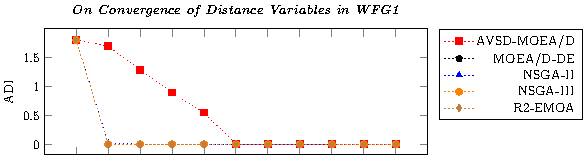
\includegraphics[scale=0.8]{images/Diversity_Long_Term_tikz_WFG1-figure0.eps}\\[0cm]%[-0.14cm] 
 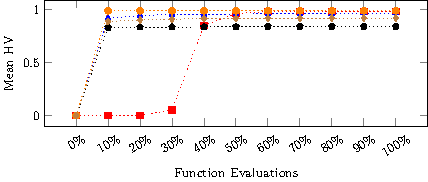
\includegraphics[scale=0.8]{images/Diversity_Long_Term_tikz_WFG1-figure1.eps}\\[0cm]%[-0.14cm] 
\end{tabular}
\caption{Diverstiy of distance variables (first row) and mean of \HV{} values (second row) vs. elapsed time in the bi-objective WFG1 test problem. The reported results are taken from $35$ runs.}\label{fig:WFG1_Diversity}
\end{figure}


\begin{figure}[t]
\centering
\begin{tabular}{l}
 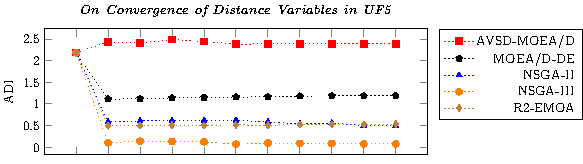
\includegraphics[scale=0.8]{images/Diversity_Long_Term_tikz_UF5-figure0.eps}\\[0cm]%[-0.14cm] 
 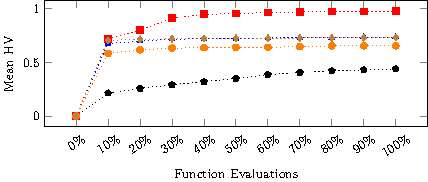
\includegraphics[scale=0.8]{images/Diversity_Long_Term_tikz_UF5-figure1.eps}\\[0cm]%[-0.14cm] 
\end{tabular}
\caption{Diverstiy of distance variables (first row) and mean of \HV{} values (second row) vs. elapsed time in the bi-objective UF5 test problem. The reported results are taken from $35$ runs.}\label{fig:UF5_Diversity}
\end{figure}

In order to better understand the benefits of \VSDMOEAD{} against the state-of-the-art \MOEAS{}.
%
This section ilustrates the evolution of the \HV{} values and the diversity of some \MOPS{}.
%
According to the \WFG{} test problems, the variables can be classified into two kinds of variables: the distance variables and the position variables.
%
Note that a variable $x_i$ is a distance variable when for all $x$, modifying $x_i$ results in a new solution that dominates $x$, is equivalent to $x$, or is dominated by $x$.
%
However, if $x_i$ is a position variable, modifying $x_i$ in $x$ always results in a vector that is incomparable or equivalent to $x$~\cite{huband2006review}.
%
Particularly, in the WFG1 the distance variables are uni-modal and its optimal region has polynomial and flat properties, which might provoke stagnation in some \MOEAS{}.
%
In contrast, the UF5 is a multi-modal problem and its optimal regions are quite isolated among the decision variable space, in fact its Pareto optimal front is discretized and conformed by only $21$ points.
%
%
For each algorithm, the selected diversity metric is calculated as the average Euclidean distance among individuals (\ADI{}) in the population by considering only the distance variables.
%
Figures~\ref{fig:WFG1_Diversity} and~\ref{fig:UF5_Diversity} show how the ADI (top) and the mean of \HV{} (bottom) evolve for the WFG1 and UF5, respectively.
%
In the WFG1 problem, the distance variables of the state-of-the-art \MOEAS{} converged to a region approximately after the $10\%$ of the total execution.
%
Among the remaining function evaluations those \MOEAS{} were not able to improve the quality of its approximations.
%
In the case of \VSDMOEAD{}, the decrease in \ADI{} is quite linear until the halfway point of the execution.
%
Showing that preserving diversity at different levels might improve the final approximation.
%
Although \RMOEA{} attained the best \HV{} values in several problems, its degradation in some problems (e.g. WFG1) is quite shocking.
%
This is not the case of \VSDMOEAD{}, whose performance was always the best or almost the best.
%

Promoting explicitly diversity among the execution is also benefical to multi-modal problems.
%
For instance, the advantage of promoting diversity in the UF5 test problem is shown in Figure~\ref{fig:UF5_Diversity}.
%
Particularly, this figure shows that \VSDMOEAD{} not only attained a better \HV{} values at the first $10\%$ of total function evaluations, it also kept looking for promising regions.
%
In fact, its \HV{} values improved meaningfully until a half of total execution that is the final point in which the diversity were explicitly promoted.
%
It also shows that \MOEADDE{} finds several promising regions among the execution, such effect might be provoked by the polynomial mutation.
%
Nevertheless, the improvements provoked by this operator does not improve two state-of-the-art \MOEAS{} at the end of the execution.
%
The reamining \MOEAS{} reported the same \HV{} and \ADI{} values after $10\%$ of the total function evaluations.


\subsection{Decision Variable Scalability Analysis}

In order, to have a better insight of the benefits of our proposal, the scalability in term of the number of decision variables is tested.
%
In particular, this experiment was carried out with the decomposition-based algorithms.
%
Such \MOEAS{} were applied with the same benchmark problems, but considering $50$, $100$, $250$ and $500$ variables.
%
Note that in the WFG test problems, the number of position variables and distance variables must be specified.
%
Specifically, the number of distance variables was set to $42$, $84$, $210$ and $418$ when using $50$, $100$, $250$ and $500$ variables, respectively.
%
%The remaining variables were the position variables, whose number was set to $8$, $16$, $40$ and $82$, respectively.
The rest of the decision variables were position variables, meaning that they were $8$, $16$, $40$ and $82$, respectively.
%
In addition, the stopping criterion was set to $2.5 \times 10^7$ function evaluations.
%
Figures~\ref{fig:scalability-2obj} and~\ref{fig:scalability-3obj} show the mean \HV{} ratio for the selected algorithms, considering the problems with two and three objectives, respectively.
%
In spite that the \HV{} ratio decreases as the number of variables increases, with two and three objectives the performance of \VSDMOEAD{} is quite robust, in fact its deterioration is much lower than \MOEADDE{}.
%

\begin{figure}[t]
\centering
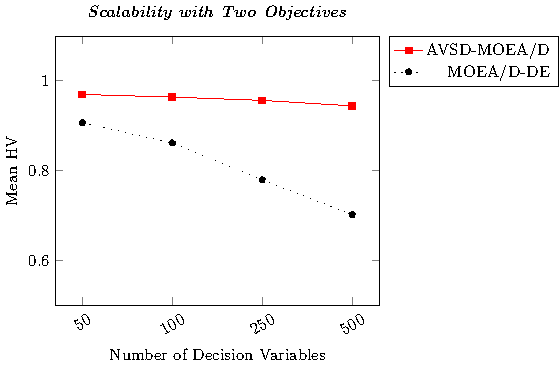
\includegraphics[scale=0.85]{images/Graphic-Scalability-2obj_tikz-figure0.eps}
\caption{Mean of the \HV{} ratio for 35 runs for the two-objective problems considering different numbers of variables}\label{fig:scalability-2obj}
\end{figure}

\begin{figure}[t]
\centering
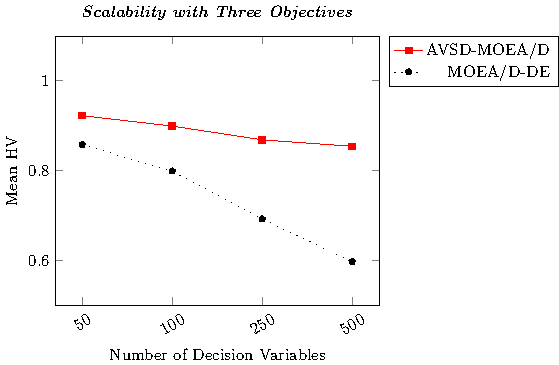
\includegraphics[scale=0.85]{images/Graphic-Scalability-3obj_tikz-figure0.eps}
\caption{Mean of the \HV{} ratio for 35 runs for the three-objective problems considering different numbers of variables} \label{fig:scalability-3obj}
\end{figure}


\begin{figure}[t]
\centering
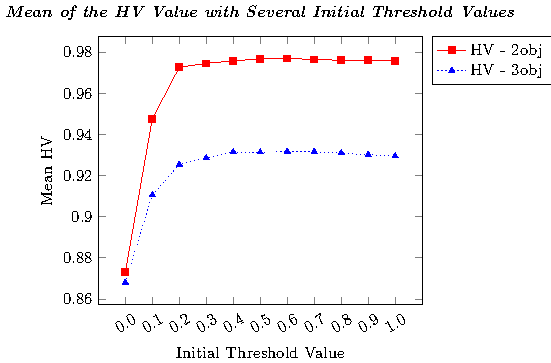
\includegraphics[scale=0.85]{images/Graphic-Initial-Distance_tikz-figure0.eps} \\
\caption{Mean of \HV{} values taking into account all the problems with several initial threshold values}\label{fig:Initial-distance-factor}
\end{figure}


\subsection{Analysis of the Initial Threshold Value}

Possibly, the main downside of including a strategy to explicitly promoting the diversity is the need of incorporating an additional parameter.
%
For instance, \VSDMOEAD{} requires to set an initial threshold value ($D_I)$.
%
Given the evidence of several findings in the literature, in the previous experiments a value of $D_I=0.4$ was used.
%
However, in this section a more detailed study of this parameter is driven.
%

%
In this section is analized the overall performance of \VSDMOEAD{} using different $D_I$ values.
%
Thereafter, in a more specifically way, the effect of this parameter is analized in WFG9 and UF10 test problems, in two and three objectives, respectively.
%
Note that, since normalized distances are used, the maximum difference that can appear is $1.0$, which belongs to the main diagonal of the box-constrained minimization \MOP{}.
%
Additionally, note that when $D_I$ is set to $0.0$, no individual is penalized on the basis of its decision variable space diversity contribution, so \VSDMOEA{} would behave like a more traditional \MOEA{}.
%
Specifically, the values $D_I = \{0.0, 0.1, 0.2, 0.3, 0.4, 0.5, 0.6, 0.7, 0.8, 0.9, 1.0\}$ were tested.
%
As in previous experiments, the whole set of benchmark problems was used and the stopping criterion was set to $2.5 \times 10^7$ function evaluations.

Figure~\ref{fig:Initial-distance-factor} shows the mean \HV{} ratio obtained for both the two-objective  and the three-objective case.
%

The worst performance of the \VSDMOEAD{} is when it is set to $D_I=0.0$.
%
The \HV{} ratio obtained quickly increases as higher $D_I$ values up to $0.2$ are used.
%
Larger values provide a quite similar performance.
%
In fact, there is a wide range of values (from $0.2$ to $1.0$) where the performance is very good, meaning that the behavior of \VSDMOEA{} is quite robust.
%
Thus, properly setting this parameter is not a complex task.
%

In the same way than in the previous experiments, the Figures~\ref{fig:WFG9_Diversity} and~\ref{fig:UF10_Diversity} show the evolution of diversity (top side) and \HV{} ratio (bottom side) among the execution.
%
The WFG9 test problem is multi-modal and deceptive.
%
In addition, the UF10 test problem is highly multi-frontal and can be considered as one of the most challenging problems.
%
Such diagrams belong to \VSDMOEAD{} with the values $D_I = \{0.0, 0.4, 1.0\}$.
%
Interestingly, the behavior of \VSDMOEAD{} with $D_I=0.0$ is quite similar than the state-of-the-art \MOEAS{}, which confirms or previous claim.
%
The motivation behind those diagrams is to ilustrate that to achieve a better balance between exploration and exploitation can be the explicit promotion of diversity among the execution.
%
Therefore, those figures show that in multi-objective optimization --depending in each \MOP{}-- there is a relation between the diversity and the quality solutions, in fact visually the shapes of the \ADI{} and \HV{} ratio complement each other.
%
Even more the \HV{} ratio values are constantly improving as the execution time elapses.
%

\begin{figure}[t]
\centering
\begin{tabular}{l}
 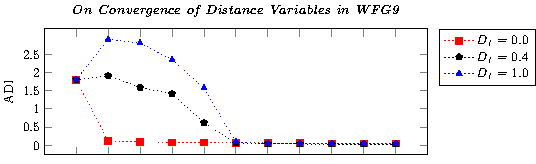
\includegraphics[scale=0.8]{images/Diversity_Long_Term_tikz_WFG9-figure0.eps}\\[0cm]%[-0.14cm] 
 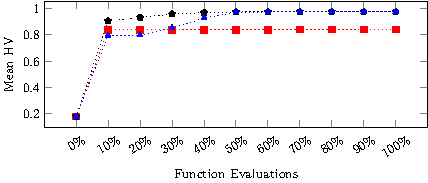
\includegraphics[scale=0.8]{images/Diversity_Long_Term_tikz_WFG9-figure1.eps}\\[0cm]%[-0.14cm] 
\end{tabular}
\caption{Diverstiy of distance variables (first row) and mean of \HV{} values (second row) vs. elapsed time in the two-objective WFG9 test problem. The reported results are taken from $35$ runs.}\label{fig:WFG9_Diversity}
\end{figure}


\begin{figure}[t]
\centering
\begin{tabular}{l}
 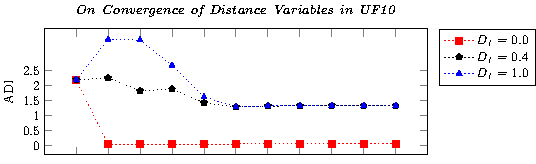
\includegraphics[scale=0.8]{images/Diversity_Long_Term_tikz_UF10-figure0.eps}\\[0cm]%[-0.14cm] 
 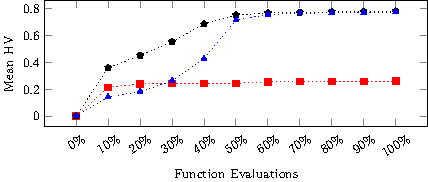
\includegraphics[scale=0.8]{images/Diversity_Long_Term_tikz_UF10-figure1.eps}\\[0cm]%[-0.14cm] 
\end{tabular}
\caption{Diverstiy of distance variables (first row) and mean of \HV{} values (second row) vs. elapsed time in the three-objective UF10 test problem. The reported results are taken from $35$ runs.}\label{fig:UF10_Diversity}
\end{figure}



\section{Conclusion}
\label{Sec:Conclusion}
Premature convergence is one of the most typical drawbacks of \EAS{}.
%
\MOEAS{} promote indirectly the preservation of diversity on variable space
because of the explicit maintenance of diversity on objective space.
%
However, for many problems the degree of diversity maintained is not enough to keep the exploration
power and locate the optimal regions.
%
In single-objective optimization, many of the state-of-the-art algorithms consider an explicit management of
diversity.
%
Particularly, those schemes that relate the degree of diversity with the elapsed period and stopping criterion
have excelled.
%
This paper shows that this design principle is also helpful for the multi-objective optimization area,
where the optimization of many of the most complex popular benchmark problems can be improved further
by applying this design principle.

In order to prove previous hypothesis, a novel replacement operator based on the aforementioned design principle
is integrated to generate a decomposition-based \MOEA{} that takes into account the diversity of both variable 
space and objective function space.
%
This is performed using a dynamic penalty method. 
%
Note that since the aim of the approach is to improve the results when considering metrics of the objective space,
the importance given to the diversity on the variable space is reduced as the evolution progresses, meaning that
at later phases our proposal behaves more similarly to traditional \MOEAS{}.
%
Additionally, taking into account some of the recent advances in the area and that our proposal might not maintain
some high-quality solutions in the population because of the penalty scheme, an external archive based on the
R2-indicator is incorporated.
%
As a result our proposal is referred to as \AVSDMOEAD{}.
%

The experimental validation carried out shows the remarkable improvement provided by \AVSDMOEAD{} in comparison to
state-of-the-art \MOEAS{} both in two-objective and three-objective problems.
%
The scalability analyses show that as the number of decision variables increases the benefits of including
a proper management of diversity is even more important, so the differences in performance increases.
%
In fact, the most remarkable benefits appear for the most complex cases.
%
Additionally, the analysis of the initial penalty threshold, which is an additional parameter required by \AVSDMOEAD{}, 
shows that the method is quite robust so finding a proper parameter value is not a difficult task.
%
Finally, in order to better understand the reasons behind the huge superiority of the proposal, some analyses regarding
the dynamics of the populations are provided.

In the future we plan to apply the principles studied in this paper to other categories of \MOEAS{}.
%
For instance, including the diversity management put forth in this paper in indicator-based \MOEAS{} seems plausible.
%
Additionally, in order to obtain even better results, these strategies are going to be incorporated with continuation and/or individual
improvement methods.


\section*{Acknowledgments}
Authors acknowledge the financial support from CONACyT through the ``Ciencia B\'asica'' project no. 285599
and the support from ``Laboratorio de Superc\'omputo del Bajio'' through the project 300832 from CONACyT.


%% The Appendices part is started with the command \appendix;
%% appendix sections are then done as normal sections
%% \appendix

%% \section{}
%% \label{}

%% References
%%
%% Following citation commands can be used in the body text:
%% Usage of \cite is as follows:
%%   \cite{key}          ==>>  [#]
%%   \cite[chap. 2]{key} ==>>  [#, chap. 2]
%%   \citet{key}         ==>>  Author [#]

%% References with bibTeX database:

% \bibliographystyle{model1-num-names}

%% New version of the num-names style
\bibliographystyle{elsarticle-num-names}
\bibliography{bibtex/References.bib}

%% Authors are advised to submit their bibtex database files. They are
%% requested to list a bibtex style file in the manuscript if they do
%% not want to use model1-num-names.bst.

%% References without bibTeX database:

% \begin{thebibliography}{00}

%% \bibitem must have the following form:
%%   \bibitem{key}...
%%

% \bibitem{}

% \end{thebibliography}


\end{document}

%%
%% End of file `elsarticle-template-1-num.tex'.
